% ###################################################################
\chapter{Addressing in Human-Robot Conversational Groups}\label{ch.meka}

\iniload{meka.info}{data/data.info_meka.ini}

\begin{displaycquote}[p. 36]{Kendon1967}
From \emph{p}'s point of view then, \emph{p} may be said to be 'offering' \emph{q} the floor, for in looking steadily at him he indicates that he is now \enquote{open} to his actions, whatever they may be.\\
\end{displaycquote}

In this chapter I investigate \Cref{hyp.meka}\rqnote{hyp.meka}{\hypmeka}.
To this end, I present a scenario in which a \gls{robot} participates in a \gls{conversational group} with multiple people in the \gls{csra} to solve tasks verbally directed at it.
The collected observations are used to evaluate an approach to \gls{addressee} recognition in multi-party \acrlong{hri}.
Finally, I discuss the results of the evaluation and the implications for the research question.

\section{Introduction}

In dyadic \gls{hri} scenarios, it can by definition be assumed that only one person interacts with the \gls{robot}.
Therefore, \glspl{robot} can assume to always be the \gls{addressee} of speech~\cite{Holthaus,Carlmeyer2014,Huang2016}.
For instance, a poll questioning \gls{robot}---presented by~\citewithauthor{Bruce2002}---pays attention to a person from the moment its \emph{area of interest} is entered and until the end of the interaction.
All other persons are ignored during that time.
However, the assumptions that \glspl{conversation} are always dyadic and that all utterances are produced to cause a verbal response from the \glsatt{conversation} partner do not hold in most interaction scenarios.
When several persons are present, they can not only speak to a \gls{robot}.
They dynamically create and change \glspl{conversational group} and converse with each other (see: \cref{sec.rw.hi.faceengagements}).
Even when the \gls{robot} knows that it is in a \gls{conversational group} and with whom\footnote{the problem of {conversational group} detection with \glspl{artificial agent} is investigated in \cref{ch.fformation}}, it still needs to actively participate in this group.
At least, it needs to know when to react to an utterance and when not.
As presented in \cref{sec.rw.hi.focused-rw.addressing}, different approaches to automatic \gls{addressee} recognition are possible.
Most of the approaches used in \gls{hri} employ information about the participants \gls{vfoa} and acoustic information to decide whether the \gls{robot} is addressed by a \gls{speaker} or not.
To distinguish which person speaks at a particular time, techniques for sound source localization or close-talk microphones are often applied~\cite{Lang2003,Skantze2014}.
In this chapter, I present a multi-party, \acrlong{hri} scenario, designed to confront the \gls{robot} with the problems of participation in a \gls{conversational group} and autonomous decision whether to react to an utterance within the group or not.
We designed this scenario, implemented it on the \gls{floka}, and applied it in an experimental study in the \gls{csra}~\cite{Richter}.
This scenario is particularly suitable for the evaluation of \gls{addressee} recognition approaches for \glspl{artificial agent}.
A description of the study set-up, recording and annotation, used platform, implemented attention and dialogue management systems, as well as an initial evaluation of the used addressing recognition can be found in the corresponding publication~\cite{Richter}.
On the basis of the collected data, I investigate \Cref{hyp.meka} by examining the following claims: 
\newcommand{\hypmekahone}{By visually observing movements of lips, an agent can recognize if a person has the role of \gls{speaker} in a \gls{conversational group}.}
\begin{hyp3}[Speaker Detection]
    \label{meka.h1}
    \hypmekahone
\end{hyp3}
\newcommand{\hypmekahtwo}{Recognizing mutual gaze with a participant of the \gls{conversational group} at the end of an utterance, can be interpreted by an agent as a prompt to take the next \gls{turn}.}
\begin{hyp3}[Next Speaker Detection]
    \label{meka.h2}
    \hypmekahtwo
\end{hyp3}
\newcommand{\hypmekahthree}{Mouth movement and gaze information about a participant of a \gls{conversational group} can be combined and put into context to recognize if a \gls{robot} is addressed with an utterance or not.}
\begin{hyp3}[Addressee Detection]
    \label{meka.h3}
    \hypmekahthree
\end{hyp3}
I investigate \Cref{hyp.meka} by incorporating these claims into an \gls{addressee} recognition system and evaluating its applicability in a multi-party \gls{hri} scenario.

\section{Human-Robot Addressing Corpus}\label{sec.meka.corpus}

The evaluation of \gls{addressee} recognition approaches in \gls{hri} poses multiple challenges to the design of the interaction.
\Gls{addressee} recognition is the distinction of utterances addressed towards the agent from utterances exchanged between other people in the situation.
Therefore, a scenario needs to be chosen that encourages both: interactions with the agent and with other people.
Furthermore, the interaction should encourage that both the speaker and the \gls{addressee} change on a regular basis and both addressing and non-addressing of the \gls{robot} can be regularly observed.
In this section, I present a \gls{hri} scenario and implemented \gls{robot} behaviour that satisfies these requirements.
Subsequently, I describe the corresponding experiment and annotation procedure.
The resulting corpus is presented at the end of this section.

\subsection{Multi-Party Interaction Scenario}\label{sec:meka-scenario}

We designed a multi-party \gls{hri} scenario in the \gls{csra} in which human participants ask a \gls{robot} questions and make it control the environment.
To this end, the participants are equipped with a set of notes, containing tasks for the \gls{robot}.
% procedure
To enforce a better balance between addressing of the \gls{robot} and other participants, a two-step communication of the tasks is performed.
The procedure is as follows:
\begin{enumerate}
    \item Participant \(P_a\) uncovers a note.
    \item \(P_a\) communicates the task to a second participant \(P_b\).
    \item \(P_b\) takes the \gls{turn} and communicates the task to the \gls{robot} \(R\).
    \item The \gls{robot} \(R\) accepts and solves the task. 
    \item \(P_b\) takes the role of \(P_a\)\footnote{Participants naturally ensure a uniform distribution of participation in the group in such a tash. This can be expected based on the literature and is confirmed in this study.}.
    \item This is repeated until all notes are uncovered. 
\end{enumerate}
The communication of the task from one participant to another not only enforces interaction between the participants.
It additionally confronts the \gls{robot} with utterances that verbally match its expectations but address someone else.
% enforced f-formation
To further support a uniform distribution of the \glspl{conversational role} in the interaction, we recommend a closed, circular \gls{conversational group} configuration.
To this end, we chose interactions with three human participants and one \gls{robot}, distributed around a table in the \gls{csra}'s living room (see \cref{fig:meka-intro}).
\begin{figure}[tbh]
    \centering
    \begin{subfigure}[t]{0.49\textwidth}
        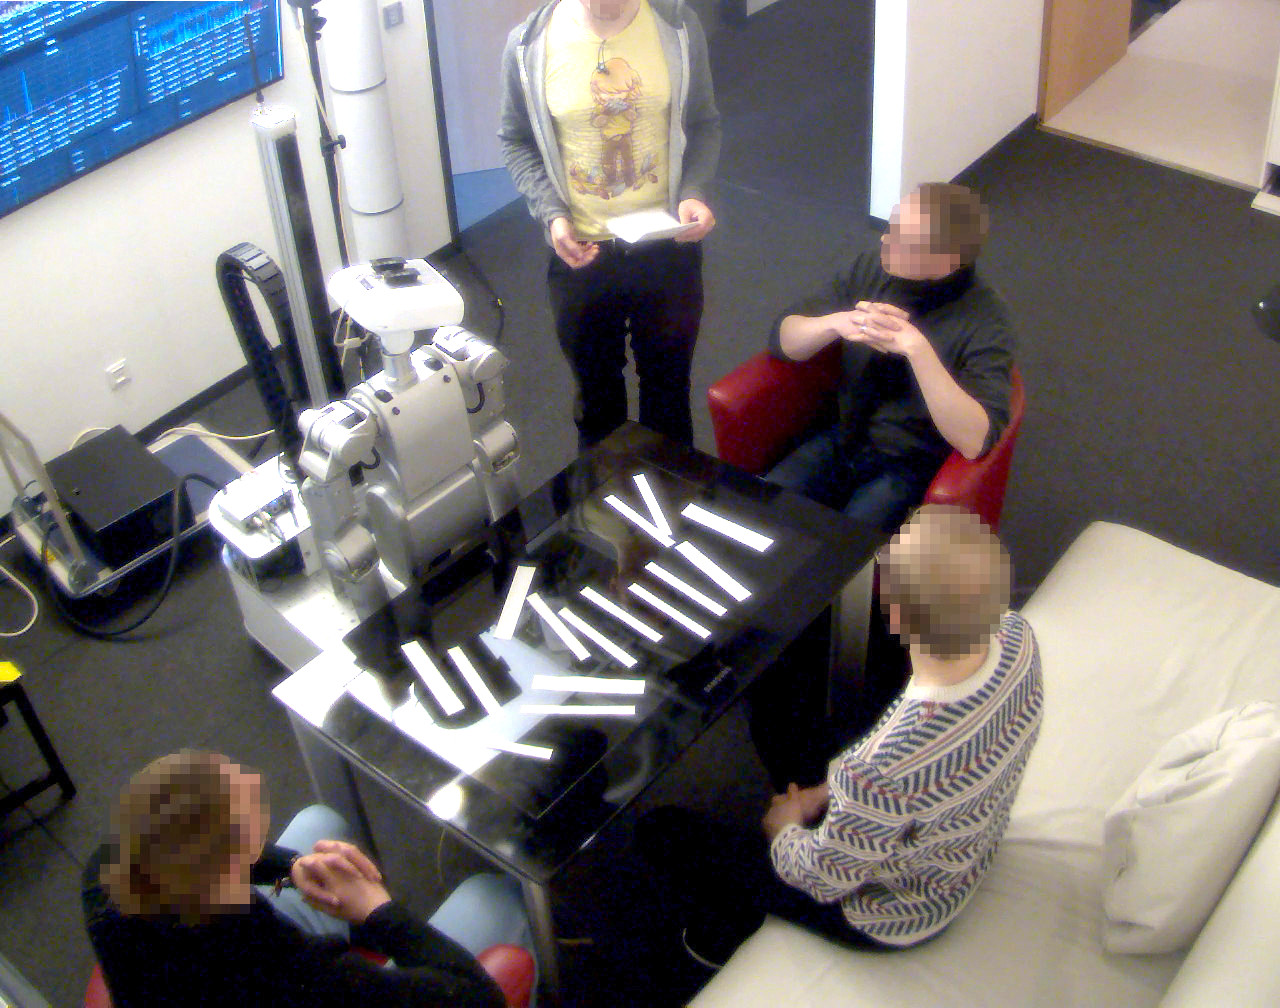
\includegraphics[trim=55 0 80 0, clip, width=\textwidth]{figures/addressee-meka-intro.jpg}
        \caption{Scene during the briefing.}
        \label{fig:meka-intro-shot}
    \end{subfigure}
    \hfill
    \begin{subfigure}[t]{0.49\textwidth}
        \def\svgwidth{1.0\textwidth}
        \input{generated/csra_map_study_meka.pdf_tex}
        \caption{Map of the study set-up.}
        \label{fig:meka-map}
    \end{subfigure}
    \caption[Configuration during robot addressing study.]{\label{fig:meka-intro}
    (a) The left image shows a scene during the briefing of participants, recorded by the camera \(C_1\).
    The participants and \gls{robot} are already correctly placed for the study.
    The experimenter is standing next to the \gls{robot} and describing the study procedure.
    (b) The right image shows a map of the \gls{apartment}'s living room during the study.
    The participants \(P_1\), \(P_2\), and \(P_3\) are seated on the armchairs and sofa (yellow).
    They and the \gls{robot} (green) surround a table (gray) on which the task notes (red) are spread.
    }
\end{figure}
This allows the participants to interact with each other and with the \gls{robot} without the need to rearrange between \glspl{turn}.
Therefore, there is no need for changes in the \gls{conversational group} arrangement.
When the interactants position themselves at the edges of the table, their resulting distribution in the \gls{pspace} of the \gls{conversational group} is uniform.
Therefore, all participants have the same access to the \gls{conversational group} and no particular distribution of roles is imposed on the interaction (see \cref{sec.rw.hi.cg}).
%  summary
With this approach we create a suitable scenario for the evaluation of \glsatt{robot} \gls{addressee} recognition with (1) a clear motivation for the participants, (2) a fixed \gls{conversational group}, and (3) a good ratio between addressing of the \gls{robot} and other participants.


\subsection{System Set-Up}
% intro and robot
Literature suggests that the behaviour of an agent influences the behaviour of participants (see \cref{sec.rw.hi.focused-rw.perception}).
Therefore, it is important to consider which behaviours of the \gls{robot} are desirable and how these may influence the course of the interaction.
We used the anthropomorphic \gls{robot} \gls{floka} with its sensor head (as presented in \vref{fig:csra-map-meka}).
The human-like upper body of the \gls{robot} allows a clear recognizability of its front, and therefore allows people to estimate its \gls{transactional segment}.
Furthermore, by turning its head---pan and tilt---the \gls{robot} can show attention. 

% attention and dialogue management
To allow \gls{floka} to actively participate in the interaction, we provided it with an attention management system.
It integrates multi-modal sensor information from the \glspl{robot} camera and microphones to direct its visual attention to salient areas.
This allows \gls{floka} to (1) focus on participants of the interaction by looking at their faces and (2) shift its attention towards a \gls{speaker} by turning towards sound sources.
The \gls{robot} continuously exhibits this attentive behaviour to provoke the impression that it is following the interaction.
Furthermore, this should allow the \gls{robot} to focus on the current \gls{speaker} of the \gls{conversational group}.
The implementation of the attention management system is presented in the corresponding publication~\cite{Richter}.
The dialogue management system, presented by~\citewithauthor{Carlmeyer2014}, utilizes the results of the \gls{addressee} recognition component to only processes utterances when the \gls{robot} considers itself addressed.
In this case the \gls{robot} implicitly takes the \gls{turn}, produces a verbal response to the recognized task, and finally yields its \gls{turn} by ending speech production and continuing with its gazing behaviour.
The \gls{addressee} recognition component is presented in detail in the following section.

\subsection{Addressee Recognition}\label{sec.meka.study.classifiers}

To investigate the \cref{meka.h1,meka.h2,meka.h3} I implemented a system for \gls{addressee} recognition that incorporates the detection of mouth movements and mutual gaze to distinguish utterances addressed towards the \gls{robot} from other utterances.
% \gls{addressee} recognition system
It combines two kinds of information (\cref{meka.h1}) whether a person is speaking, and (\cref{meka.h2}) whether this person maintains mutual gaze with the \gls{robot}.
To this end, I extended the gaze detector created by~\citewithauthor{Schillingmann2015} to make its gaze recognition results and the results of the facial landmark detection~\cite{Sagonas2013} available within the \gls{csra}.
The used features are visualized in \cref{fig:meka-features}.
\begin{figure}[htb]
    \centering
    \def\svgwidth{1.0\textwidth}
    \input{generated/meka-addressee-gzetool.pdf_tex}
    \caption[Mutual gaze and mouth movement features.]{\label{fig:meka-features}
    Visualization of the features used in the \gls{addressee} recognition.
    The person on the left maintains mutual gaze and is speaking, the person on the right does neither of it.
    The upper images show the results of the gaze recognition system---horizontal and vertical angle---from~\citewithauthor{Schillingmann2015}, augmented with the default thresholds for mutual gaze (blue bars) and the current estimation (green bars).
    The centred images show visualizations of the estimated head orientation (blue), and a red rectangle in case of mutual gaze.
    The inner corner-points of the eyes are highlighted in pink.
    The lower images show the facial landmarks (cyan lines) in the region of the mouth and highlight the central mouth landmarks (red dots) and corresponding distances (yellow lines).
    }
\end{figure}
The gaze detection provides the horizontal and vertical angle between the participants gaze direction and the image centre.
Because the \gls{robot}'s camera is located at the centre of its head, the person is looking directly into the \glspl{robot} face when both angles are zero.
Therefore, to decide whether a person \(p\) maintains mutual gaze with the \gls{robot}, I compare the magnitude of both their horizontal (\(\alpha_p\)) and vertical (\(\beta_p\)) gaze angles to a threshold \(\theta\).
\begin{equation}\label{eq:meka.mg}
    G(p) = | \alpha_p | < \theta \land | \beta_p | < \theta
\end{equation}
For the recognition of mouth movements, distances between the central points of the inner mouth (see \cref{fig:meka-features}) are observed during a sliding time window \(\Delta_t\).
This results in a set of distances \(\mathbf{D_p}\) for each person \(p\).
A person is recognized as speaking if the variance of these distances exceeds a threshold \(d\).
\begin{equation}\label{eq:meka.sp}
    S(p) = \text{Var}(\mathbf{D_p}) > d
\end{equation}
To decide whether a person \(p\) is addressing the \gls{robot} at a particular time, the results of both \cref{eq:meka.mg} and \cref{eq:meka.sp} are then combined.
\begin{equation}\label{eq:meka.ad}
    A(p) = G(p) \land S(p)
\end{equation}
The thresholds \(\theta = \ang{12}\), \(d=1.5\), and the time window \(\Delta_t=\SI{600}{\ms}\) were selected based on a pre-study with the same set-up.

\subsection{Study Procedure}

After the participants gave their consent to the recording, they were accompanied into the \gls{apartment}'s living room by the experimenter and asked to take a seat in the armchairs and sofa.
The \gls{robot} was already waiting at the table.
The following tasks were laid out on the table:
\begin{enumerate*}[label=(\roman*)]
    \item \emph{Turn the light on.}
    \item \emph{Turn the light off.}
    \item \emph{What time is it?}
    \item \emph{Has a parcel arrived?}
    \item \emph{Has anyone called?}
    \item \emph{Which data is recorded?}
    \item \emph{What exhibits are there?}
    \item \emph{What's with the garden?}
\end{enumerate*}
All tasks except \emph{Turn the light off} existed twice. 
This added up to 15 tasks to allow each participant to solve five tasks.
After the participants took a seat, the experimenter explained the task by giving an example of an iteration of the interaction (see \cref{sec:meka-scenario}).
Additionally, the participants received two hints:
(1) They need to acquire the \gls{robot}'s attention when they want to talk to it.
(2) They do not need to repeat a task more than three times when the \gls{robot} does not solve it.
When the participants had no further questions, the experimenter left the room, activated the \gls{robot}, and monitored the interaction from an adjoining room.
When all tasks were solved, the experimenter entered the room for an informal debriefing.
The typical duration of an interaction was around \SI{10}{min}, resulting in around \SI{15}{min} for the whole trial with briefing and de-briefing.

The study was performed in German, with groups of three participants at the \gls{csra}.
The 15 study participants (2 female, 13 male) were all native German \glspl{speaker} from the \gls{citec}.
The participants gave consent to the recording of audio and video material and received confectionery as compensation for their attendance.

\subsection{Contents of the Corpus}\label{sec:meka.corpus}

The recordings of the study sum up to \SI{53}{min} of multi-party \gls{hri}.
They contain overview video recordings from the camera perspectives of \(C_1\) and \(C_4\) (see \cref{fig:meka-map}), and \gls{floka}'s perspective using its head camera.
Audio data was recorded for the \gls{apartment}'s living room and hallway.
Furthermore, system events of the \gls{apartment}, the communication between the \gls{apartment} and \gls{robot}, and the internal, high-level states of the \gls{robot} were recorded.

The \gls{robot}'s speech, mouth-movement and mutual-gaze recognition results were extracted from the recordings into~\citesoft{elansrc} tiers~\cite{Bernotat2016}.
This strongly simplified the ground-truth annotation of the \gls{robot}'s \gls{addressee} recognition.
In sum, the \gls{robot} recognized \inidata{meka.info}{sum.dialogacts} dialogue acts.
A large proportion of these acts consists of confirmations and negations which were irrelevant for the task at hand and ignored by the \gls{robot}.
Therefore, the manual annotations and remaining analyses focus on the dialogue acts that had the potential of causing a response from the \gls{robot}.
These interactions were annotated with the annotation tool~\cite{elansrc} to manually distinguish whether
\begin{enumerate*}[label=(\roman*)]
    \item the \gls{robot} was looked at by the focused person,
    \item the focused person was speaking,
    \item the \gls{robot} was addressed, and
    \item the \gls{robot} was looking at the wrong person (not the \gls{speaker})
\end{enumerate*}
at the moment the speech act was recognized by the \gls{robot}.
The resulting corpus consists of \inidata{meka.info}{sum.entries} dialogue acts that were recognized by the \gls{robot} as task relevant.
The sum of utterances addressed at the \gls{robot} can be expected to be at least the number of trials times the number of repetitions of the task.
Additionally, recognized tasks can stem from communication between the participants, repetitions, and mis-classifications of tasks.
Similarly, mis-classifications can result in tasks being recognized less often than expected.
The overall distribution of these tasks, the expected number of addressing, and the proportion of tasks addressed to the \gls{robot} can be seen in \cref{fig:meka-da-counts}.
\begin{figure}[htb]
    \centering
    % Created by tikzDevice version 0.12
% !TEX encoding = UTF-8 Unicode
\begin{tikzpicture}[x=1pt,y=1pt]
\definecolor{fillColor}{RGB}{255,255,255}
\path[use as bounding box,fill=fillColor,fill opacity=0.00] (0,0) rectangle (288.00,124.59);
\begin{scope}
\path[clip] (  0.00,  0.00) rectangle (288.00,124.59);
\definecolor{drawColor}{RGB}{255,255,255}
\definecolor{fillColor}{RGB}{255,255,255}

\path[draw=drawColor,line width= 0.6pt,line join=round,line cap=round,fill=fillColor] (  0.00,  0.00) rectangle (288.00,124.59);
\end{scope}
\begin{scope}
\path[clip] (110.65, 30.86) rectangle (217.04,119.09);
\definecolor{fillColor}{gray}{0.92}

\path[fill=fillColor] (110.65, 30.86) rectangle (217.04,119.09);
\definecolor{drawColor}{RGB}{255,255,255}

\path[draw=drawColor,line width= 0.3pt,line join=round] (133.07, 30.86) --
	(133.07,119.09);

\path[draw=drawColor,line width= 0.3pt,line join=round] (168.24, 30.86) --
	(168.24,119.09);

\path[draw=drawColor,line width= 0.3pt,line join=round] (203.41, 30.86) --
	(203.41,119.09);

\path[draw=drawColor,line width= 0.6pt,line join=round] (110.65, 37.32) --
	(217.04, 37.32);

\path[draw=drawColor,line width= 0.6pt,line join=round] (110.65, 48.08) --
	(217.04, 48.08);

\path[draw=drawColor,line width= 0.6pt,line join=round] (110.65, 58.84) --
	(217.04, 58.84);

\path[draw=drawColor,line width= 0.6pt,line join=round] (110.65, 69.60) --
	(217.04, 69.60);

\path[draw=drawColor,line width= 0.6pt,line join=round] (110.65, 80.36) --
	(217.04, 80.36);

\path[draw=drawColor,line width= 0.6pt,line join=round] (110.65, 91.11) --
	(217.04, 91.11);

\path[draw=drawColor,line width= 0.6pt,line join=round] (110.65,101.87) --
	(217.04,101.87);

\path[draw=drawColor,line width= 0.6pt,line join=round] (110.65,112.63) --
	(217.04,112.63);

\path[draw=drawColor,line width= 0.6pt,line join=round] (115.49, 30.86) --
	(115.49,119.09);

\path[draw=drawColor,line width= 0.6pt,line join=round] (150.66, 30.86) --
	(150.66,119.09);

\path[draw=drawColor,line width= 0.6pt,line join=round] (185.83, 30.86) --
	(185.83,119.09);
\definecolor{fillColor}{RGB}{55,126,184}

\path[fill=fillColor] (115.49, 32.48) rectangle (133.07, 42.16);
\definecolor{fillColor}{RGB}{228,26,28}

\path[fill=fillColor] (133.07, 32.48) rectangle (138.35, 42.16);
\definecolor{fillColor}{RGB}{55,126,184}

\path[fill=fillColor] (115.49, 43.24) rectangle (131.31, 52.92);
\definecolor{fillColor}{RGB}{228,26,28}

\path[fill=fillColor] (131.31, 43.24) rectangle (133.07, 52.92);
\definecolor{fillColor}{RGB}{55,126,184}

\path[fill=fillColor] (115.49, 53.99) rectangle (129.56, 63.68);

\path[fill=fillColor] (115.49, 64.75) rectangle (138.35, 74.44);
\definecolor{fillColor}{RGB}{228,26,28}

\path[fill=fillColor] (138.35, 64.75) rectangle (140.11, 74.44);
\definecolor{fillColor}{RGB}{55,126,184}

\path[fill=fillColor] (115.49, 75.51) rectangle (143.62, 85.20);
\definecolor{fillColor}{RGB}{228,26,28}

\path[fill=fillColor] (143.62, 75.51) rectangle (159.45, 85.20);
\definecolor{fillColor}{RGB}{55,126,184}

\path[fill=fillColor] (115.49, 86.27) rectangle (175.28, 95.96);
\definecolor{fillColor}{RGB}{228,26,28}

\path[fill=fillColor] (175.28, 86.27) rectangle (212.20, 95.96);
\definecolor{fillColor}{RGB}{55,126,184}

\path[fill=fillColor] (115.49, 97.03) rectangle (138.35,106.72);
\definecolor{fillColor}{RGB}{228,26,28}

\path[fill=fillColor] (138.35, 97.03) rectangle (147.14,106.72);
\definecolor{fillColor}{RGB}{55,126,184}

\path[fill=fillColor] (115.49,107.79) rectangle (166.48,117.47);
\definecolor{fillColor}{RGB}{228,26,28}

\path[fill=fillColor] (166.48,107.79) rectangle (173.52,117.47);
\definecolor{drawColor}{RGB}{0,0,0}

\path[draw=drawColor,line width= 0.6pt,line join=round] (133.07, 33.99) --
	(133.07, 40.64);

\path[draw=drawColor,line width= 0.6pt,line join=round] (133.07, 37.32) --
	(133.07, 37.32);

\path[draw=drawColor,line width= 0.6pt,line join=round] (133.07, 33.99) --
	(133.07, 40.64);

\path[draw=drawColor,line width= 0.6pt,line join=round] (133.07, 33.99) --
	(133.07, 40.64);

\path[draw=drawColor,line width= 0.6pt,line join=round] (133.07, 37.32) --
	(133.07, 37.32);

\path[draw=drawColor,line width= 0.6pt,line join=round] (133.07, 33.99) --
	(133.07, 40.64);

\path[draw=drawColor,line width= 0.6pt,line join=round] (133.07, 44.75) --
	(133.07, 51.40);

\path[draw=drawColor,line width= 0.6pt,line join=round] (133.07, 48.08) --
	(133.07, 48.08);

\path[draw=drawColor,line width= 0.6pt,line join=round] (133.07, 44.75) --
	(133.07, 51.40);

\path[draw=drawColor,line width= 0.6pt,line join=round] (133.07, 44.75) --
	(133.07, 51.40);

\path[draw=drawColor,line width= 0.6pt,line join=round] (133.07, 48.08) --
	(133.07, 48.08);

\path[draw=drawColor,line width= 0.6pt,line join=round] (133.07, 44.75) --
	(133.07, 51.40);

\path[draw=drawColor,line width= 0.6pt,line join=round] (133.07, 55.51) --
	(133.07, 62.16);

\path[draw=drawColor,line width= 0.6pt,line join=round] (133.07, 58.84) --
	(133.07, 58.84);

\path[draw=drawColor,line width= 0.6pt,line join=round] (133.07, 55.51) --
	(133.07, 62.16);

\path[draw=drawColor,line width= 0.6pt,line join=round] (133.07, 66.27) --
	(133.07, 72.92);

\path[draw=drawColor,line width= 0.6pt,line join=round] (133.07, 69.60) --
	(133.07, 69.60);

\path[draw=drawColor,line width= 0.6pt,line join=round] (133.07, 66.27) --
	(133.07, 72.92);

\path[draw=drawColor,line width= 0.6pt,line join=round] (133.07, 66.27) --
	(133.07, 72.92);

\path[draw=drawColor,line width= 0.6pt,line join=round] (133.07, 69.60) --
	(133.07, 69.60);

\path[draw=drawColor,line width= 0.6pt,line join=round] (133.07, 66.27) --
	(133.07, 72.92);

\path[draw=drawColor,line width= 0.6pt,line join=round] (124.28, 77.03) --
	(124.28, 83.68);

\path[draw=drawColor,line width= 0.6pt,line join=round] (124.28, 80.36) --
	(124.28, 80.36);

\path[draw=drawColor,line width= 0.6pt,line join=round] (124.28, 77.03) --
	(124.28, 83.68);

\path[draw=drawColor,line width= 0.6pt,line join=round] (124.28, 77.03) --
	(124.28, 83.68);

\path[draw=drawColor,line width= 0.6pt,line join=round] (124.28, 80.36) --
	(124.28, 80.36);

\path[draw=drawColor,line width= 0.6pt,line join=round] (124.28, 77.03) --
	(124.28, 83.68);

\path[draw=drawColor,line width= 0.6pt,line join=round] (133.07, 87.79) --
	(133.07, 94.44);

\path[draw=drawColor,line width= 0.6pt,line join=round] (133.07, 91.11) --
	(133.07, 91.11);

\path[draw=drawColor,line width= 0.6pt,line join=round] (133.07, 87.79) --
	(133.07, 94.44);

\path[draw=drawColor,line width= 0.6pt,line join=round] (133.07, 87.79) --
	(133.07, 94.44);

\path[draw=drawColor,line width= 0.6pt,line join=round] (133.07, 91.11) --
	(133.07, 91.11);

\path[draw=drawColor,line width= 0.6pt,line join=round] (133.07, 87.79) --
	(133.07, 94.44);

\path[draw=drawColor,line width= 0.6pt,line join=round] (133.07, 98.55) --
	(133.07,105.20);

\path[draw=drawColor,line width= 0.6pt,line join=round] (133.07,101.87) --
	(133.07,101.87);

\path[draw=drawColor,line width= 0.6pt,line join=round] (133.07, 98.55) --
	(133.07,105.20);

\path[draw=drawColor,line width= 0.6pt,line join=round] (133.07, 98.55) --
	(133.07,105.20);

\path[draw=drawColor,line width= 0.6pt,line join=round] (133.07,101.87) --
	(133.07,101.87);

\path[draw=drawColor,line width= 0.6pt,line join=round] (133.07, 98.55) --
	(133.07,105.20);

\path[draw=drawColor,line width= 0.6pt,line join=round] (133.07,109.31) --
	(133.07,115.96);

\path[draw=drawColor,line width= 0.6pt,line join=round] (133.07,112.63) --
	(133.07,112.63);

\path[draw=drawColor,line width= 0.6pt,line join=round] (133.07,109.31) --
	(133.07,115.96);

\path[draw=drawColor,line width= 0.6pt,line join=round] (133.07,109.31) --
	(133.07,115.96);

\path[draw=drawColor,line width= 0.6pt,line join=round] (133.07,112.63) --
	(133.07,112.63);

\path[draw=drawColor,line width= 0.6pt,line join=round] (133.07,109.31) --
	(133.07,115.96);
\end{scope}
\begin{scope}
\path[clip] (  0.00,  0.00) rectangle (288.00,124.59);
\definecolor{drawColor}{RGB}{0,0,0}

\node[text=drawColor,anchor=base east,inner sep=0pt, outer sep=0pt, scale=  1.00] at (105.70, 33.87) {Call Request};

\node[text=drawColor,anchor=base east,inner sep=0pt, outer sep=0pt, scale=  1.00] at (105.70, 44.63) {Data Request};

\node[text=drawColor,anchor=base east,inner sep=0pt, outer sep=0pt, scale=  1.00] at (105.70, 55.39) {Exhibits request};

\node[text=drawColor,anchor=base east,inner sep=0pt, outer sep=0pt, scale=  1.00] at (105.70, 66.15) {Garden Request};

\node[text=drawColor,anchor=base east,inner sep=0pt, outer sep=0pt, scale=  1.00] at (105.70, 76.91) {Light Off};

\node[text=drawColor,anchor=base east,inner sep=0pt, outer sep=0pt, scale=  1.00] at (105.70, 87.67) {Light On};

\node[text=drawColor,anchor=base east,inner sep=0pt, outer sep=0pt, scale=  1.00] at (105.70, 98.43) {Parcel Request};

\node[text=drawColor,anchor=base east,inner sep=0pt, outer sep=0pt, scale=  1.00] at (105.70,109.19) {Time Request};
\end{scope}
\begin{scope}
\path[clip] (  0.00,  0.00) rectangle (288.00,124.59);
\definecolor{drawColor}{gray}{0.20}

\path[draw=drawColor,line width= 0.6pt,line join=round] (107.90, 37.32) --
	(110.65, 37.32);

\path[draw=drawColor,line width= 0.6pt,line join=round] (107.90, 48.08) --
	(110.65, 48.08);

\path[draw=drawColor,line width= 0.6pt,line join=round] (107.90, 58.84) --
	(110.65, 58.84);

\path[draw=drawColor,line width= 0.6pt,line join=round] (107.90, 69.60) --
	(110.65, 69.60);

\path[draw=drawColor,line width= 0.6pt,line join=round] (107.90, 80.36) --
	(110.65, 80.36);

\path[draw=drawColor,line width= 0.6pt,line join=round] (107.90, 91.11) --
	(110.65, 91.11);

\path[draw=drawColor,line width= 0.6pt,line join=round] (107.90,101.87) --
	(110.65,101.87);

\path[draw=drawColor,line width= 0.6pt,line join=round] (107.90,112.63) --
	(110.65,112.63);
\end{scope}
\begin{scope}
\path[clip] (  0.00,  0.00) rectangle (288.00,124.59);
\definecolor{drawColor}{gray}{0.20}

\path[draw=drawColor,line width= 0.6pt,line join=round] (115.49, 28.11) --
	(115.49, 30.86);

\path[draw=drawColor,line width= 0.6pt,line join=round] (150.66, 28.11) --
	(150.66, 30.86);

\path[draw=drawColor,line width= 0.6pt,line join=round] (185.83, 28.11) --
	(185.83, 30.86);
\end{scope}
\begin{scope}
\path[clip] (  0.00,  0.00) rectangle (288.00,124.59);
\definecolor{drawColor}{RGB}{0,0,0}

\node[text=drawColor,anchor=base,inner sep=0pt, outer sep=0pt, scale=  1.00] at (115.49, 19.03) {0};

\node[text=drawColor,anchor=base,inner sep=0pt, outer sep=0pt, scale=  1.00] at (150.66, 19.03) {20};

\node[text=drawColor,anchor=base,inner sep=0pt, outer sep=0pt, scale=  1.00] at (185.83, 19.03) {40};
\end{scope}
\begin{scope}
\path[clip] (  0.00,  0.00) rectangle (288.00,124.59);
\definecolor{drawColor}{RGB}{0,0,0}

\node[text=drawColor,anchor=base,inner sep=0pt, outer sep=0pt, scale=  1.00] at (163.85,  7.44) {Summed recognitions};
\end{scope}
\begin{scope}
\path[clip] (  0.00,  0.00) rectangle (288.00,124.59);
\definecolor{drawColor}{RGB}{0,0,0}

\node[text=drawColor,rotate= 90.00,anchor=base,inner sep=0pt, outer sep=0pt, scale=  1.00] at ( 12.39, 74.98) {Dialogue Acts};
\end{scope}
\begin{scope}
\path[clip] (  0.00,  0.00) rectangle (288.00,124.59);
\definecolor{fillColor}{RGB}{255,255,255}

\path[fill=fillColor] (228.04, 48.11) rectangle (282.50,101.85);
\end{scope}
\begin{scope}
\path[clip] (  0.00,  0.00) rectangle (288.00,124.59);
\definecolor{drawColor}{RGB}{0,0,0}

\node[text=drawColor,anchor=base west,inner sep=0pt, outer sep=0pt, scale=  1.00] at (233.54, 88.49) {Addressee};
\end{scope}
\begin{scope}
\path[clip] (  0.00,  0.00) rectangle (288.00,124.59);
\definecolor{drawColor}{RGB}{255,255,255}
\definecolor{fillColor}{gray}{0.95}

\path[draw=drawColor,line width= 0.6pt,line join=round,line cap=round,fill=fillColor] (233.54, 68.06) rectangle (247.99, 82.51);
\end{scope}
\begin{scope}
\path[clip] (  0.00,  0.00) rectangle (288.00,124.59);
\definecolor{fillColor}{RGB}{228,26,28}

\path[fill=fillColor] (234.25, 68.77) rectangle (247.28, 81.80);
\end{scope}
\begin{scope}
\path[clip] (  0.00,  0.00) rectangle (288.00,124.59);
\definecolor{drawColor}{RGB}{255,255,255}
\definecolor{fillColor}{gray}{0.95}

\path[draw=drawColor,line width= 0.6pt,line join=round,line cap=round,fill=fillColor] (233.54, 53.61) rectangle (247.99, 68.06);
\end{scope}
\begin{scope}
\path[clip] (  0.00,  0.00) rectangle (288.00,124.59);
\definecolor{fillColor}{RGB}{55,126,184}

\path[fill=fillColor] (234.25, 54.32) rectangle (247.28, 67.35);
\end{scope}
\begin{scope}
\path[clip] (  0.00,  0.00) rectangle (288.00,124.59);
\definecolor{drawColor}{RGB}{0,0,0}

\node[text=drawColor,anchor=base west,inner sep=0pt, outer sep=0pt, scale=  0.80] at (252.99, 72.53) {Other};
\end{scope}
\begin{scope}
\path[clip] (  0.00,  0.00) rectangle (288.00,124.59);
\definecolor{drawColor}{RGB}{0,0,0}

\node[text=drawColor,anchor=base west,inner sep=0pt, outer sep=0pt, scale=  0.80] at (252.99, 58.08) {Robot};
\end{scope}
\end{tikzpicture}

    \vspace{-25pt}
    \caption[Recognized dialogue acts during the study.]{\label{fig:meka-da-counts}
    This plot shows how often each relevant dialogue act was recognized by the \gls{robot} during the study over all trials.
    The utterances that were addressed at the \gls{robot} are highlighted in blue, the other in red.
    A black, horizontal line shows the amount of tasks that were expected to be addressed at the \gls{robot} during the trials.
    }
\end{figure}
As apparent in \cref{fig:meka-da-counts}, the amount of recognized \emph{light} and \emph{time} tasks is much higher than expected while \emph{exhibits} and \emph{data} requests happened less frequent than expected.
This is mainly because these utterances often were wrongfully understood as \emph{light} and \emph{time} requests.

%\section{Recognizing a Robots Conversational Role}\label{sec:meka.evaluation}

The corpus provides observations of \gls{hri} and a ground truth annotation of whether a focused person was speaking, looking at the \gls{robot}, and whether the \gls{robot} was addressed at the time of a recognized dialogue act.
In the following sections I use this data to assess the claims stated for this chapter.

\section{Visual Speaker Detection}\label{sec:meka.h1}

% h1: Whether a person has the role of \gls{speaker} in a \gls{conversational group} can be visually recognized by observing movements of the persons lips.
In \cref{meka.h1}, I suggest that a person can be visually identified as having the role of \gls{speaker} by observing mouth movements.
The corresponding model is defined in \cref{eq:meka.sp}, and applied during the user study.
For the evaluation of visual speaker detection, I call this model the \emph{study-model}.
Additionally, I create an \emph{accept-all-model} that always assumes that the focused person has the \gls{speaker} role.
This is a reasonable approach because a proportion of \inidata{meka.info}{prev.mouthmovements} (\gls{prevalence}) of the observations shows a speaking focused person.
On the basis of the relevant utterances, recognized during the study, and the created ground truth annotations, I assess the models' performances.
To this end, I calculate their \gls{precision}, \gls{recall}, and \gls{accuracy} with 95\% confidence intervals according to~\citewithauthor{clopper1934}\footnote{Using \code{binom.test} from the \code{stats} package (v3.5.1) in R~\cite{stats}.} and \gls{f1score} as commonly used measurements for classifier performance.
To account for the \gls{prevalence} of the data, I additionally calculate the measurements \gls{markedness}, \gls{informedness}, and \gls{dor}.
The results are visualized in \cref{fig:meka-perf-mouth}.

\begin{figure}[htb]
    \centering
    % Created by tikzDevice version 0.12
% !TEX encoding = UTF-8 Unicode
\begin{tikzpicture}[x=1pt,y=1pt]
\definecolor{fillColor}{RGB}{255,255,255}
\path[use as bounding box,fill=fillColor,fill opacity=0.00] (0,0) rectangle (336.00,145.35);
\begin{scope}
\path[clip] (  0.00,  0.00) rectangle (336.00,145.35);
\definecolor{drawColor}{RGB}{255,255,255}
\definecolor{fillColor}{RGB}{255,255,255}

\path[draw=drawColor,line width= 0.6pt,line join=round,line cap=round,fill=fillColor] (  0.00,  0.00) rectangle (336.00,145.35);
\end{scope}
\begin{scope}
\path[clip] ( 28.22, 57.73) rectangle ( 64.56,123.60);
\definecolor{fillColor}{gray}{0.92}

\path[fill=fillColor] ( 28.22, 57.73) rectangle ( 64.56,123.60);
\definecolor{drawColor}{RGB}{255,255,255}

\path[draw=drawColor,line width= 0.3pt,line join=round] ( 28.22, 68.21) --
	( 64.56, 68.21);

\path[draw=drawColor,line width= 0.3pt,line join=round] ( 28.22, 83.18) --
	( 64.56, 83.18);

\path[draw=drawColor,line width= 0.3pt,line join=round] ( 28.22, 98.15) --
	( 64.56, 98.15);

\path[draw=drawColor,line width= 0.3pt,line join=round] ( 28.22,113.12) --
	( 64.56,113.12);

\path[draw=drawColor,line width= 0.6pt,line join=round] ( 28.22, 60.72) --
	( 64.56, 60.72);

\path[draw=drawColor,line width= 0.6pt,line join=round] ( 28.22, 75.69) --
	( 64.56, 75.69);

\path[draw=drawColor,line width= 0.6pt,line join=round] ( 28.22, 90.67) --
	( 64.56, 90.67);

\path[draw=drawColor,line width= 0.6pt,line join=round] ( 28.22,105.64) --
	( 64.56,105.64);

\path[draw=drawColor,line width= 0.6pt,line join=round] ( 28.22,120.61) --
	( 64.56,120.61);

\path[draw=drawColor,line width= 0.6pt,line join=round] ( 38.13, 57.73) --
	( 38.13,123.60);

\path[draw=drawColor,line width= 0.6pt,line join=round] ( 54.65, 57.73) --
	( 54.65,123.60);
\definecolor{fillColor}{RGB}{228,26,28}

\path[fill=fillColor] ( 30.70, 60.72) rectangle ( 45.56,102.57);
\definecolor{fillColor}{RGB}{55,126,184}

\path[fill=fillColor] ( 47.22, 60.72) rectangle ( 62.08,112.69);
\definecolor{drawColor}{RGB}{0,0,0}

\path[draw=drawColor,line width= 0.6pt,line join=round] ( 53.00,115.96) --
	( 56.30,115.96);

\path[draw=drawColor,line width= 0.6pt,line join=round] ( 54.65,115.96) --
	( 54.65,108.28);

\path[draw=drawColor,line width= 0.6pt,line join=round] ( 53.00,108.28) --
	( 56.30,108.28);

\path[draw=drawColor,line width= 0.6pt,line join=round] ( 36.48,106.57) --
	( 39.78,106.57);

\path[draw=drawColor,line width= 0.6pt,line join=round] ( 38.13,106.57) --
	( 38.13, 98.17);

\path[draw=drawColor,line width= 0.6pt,line join=round] ( 36.48, 98.17) --
	( 39.78, 98.17);
\end{scope}
\begin{scope}
\path[clip] ( 70.06, 57.73) rectangle (106.39,123.60);
\definecolor{fillColor}{gray}{0.92}

\path[fill=fillColor] ( 70.06, 57.73) rectangle (106.39,123.60);
\definecolor{drawColor}{RGB}{255,255,255}

\path[draw=drawColor,line width= 0.3pt,line join=round] ( 70.06, 68.21) --
	(106.39, 68.21);

\path[draw=drawColor,line width= 0.3pt,line join=round] ( 70.06, 83.18) --
	(106.39, 83.18);

\path[draw=drawColor,line width= 0.3pt,line join=round] ( 70.06, 98.15) --
	(106.39, 98.15);

\path[draw=drawColor,line width= 0.3pt,line join=round] ( 70.06,113.12) --
	(106.39,113.12);

\path[draw=drawColor,line width= 0.6pt,line join=round] ( 70.06, 60.72) --
	(106.39, 60.72);

\path[draw=drawColor,line width= 0.6pt,line join=round] ( 70.06, 75.69) --
	(106.39, 75.69);

\path[draw=drawColor,line width= 0.6pt,line join=round] ( 70.06, 90.67) --
	(106.39, 90.67);

\path[draw=drawColor,line width= 0.6pt,line join=round] ( 70.06,105.64) --
	(106.39,105.64);

\path[draw=drawColor,line width= 0.6pt,line join=round] ( 70.06,120.61) --
	(106.39,120.61);

\path[draw=drawColor,line width= 0.6pt,line join=round] ( 79.97, 57.73) --
	( 79.97,123.60);

\path[draw=drawColor,line width= 0.6pt,line join=round] ( 96.48, 57.73) --
	( 96.48,123.60);
\definecolor{fillColor}{RGB}{228,26,28}

\path[fill=fillColor] ( 72.53, 60.72) rectangle ( 87.40,120.61);
\definecolor{fillColor}{RGB}{55,126,184}

\path[fill=fillColor] ( 89.05, 60.72) rectangle (103.91,111.84);
\definecolor{drawColor}{RGB}{0,0,0}

\path[draw=drawColor,line width= 0.6pt,line join=round] ( 94.83,115.27) --
	( 98.13,115.27);

\path[draw=drawColor,line width= 0.6pt,line join=round] ( 96.48,115.27) --
	( 96.48,107.35);

\path[draw=drawColor,line width= 0.6pt,line join=round] ( 94.83,107.35) --
	( 98.13,107.35);

\path[draw=drawColor,line width= 0.6pt,line join=round] ( 78.31,120.61) --
	( 81.62,120.61);

\path[draw=drawColor,line width= 0.6pt,line join=round] ( 79.97,120.61) --
	( 79.97,118.84);

\path[draw=drawColor,line width= 0.6pt,line join=round] ( 78.31,118.84) --
	( 81.62,118.84);
\end{scope}
\begin{scope}
\path[clip] (111.89, 57.73) rectangle (148.22,123.60);
\definecolor{fillColor}{gray}{0.92}

\path[fill=fillColor] (111.89, 57.73) rectangle (148.22,123.60);
\definecolor{drawColor}{RGB}{255,255,255}

\path[draw=drawColor,line width= 0.3pt,line join=round] (111.89, 68.21) --
	(148.22, 68.21);

\path[draw=drawColor,line width= 0.3pt,line join=round] (111.89, 83.18) --
	(148.22, 83.18);

\path[draw=drawColor,line width= 0.3pt,line join=round] (111.89, 98.15) --
	(148.22, 98.15);

\path[draw=drawColor,line width= 0.3pt,line join=round] (111.89,113.12) --
	(148.22,113.12);

\path[draw=drawColor,line width= 0.6pt,line join=round] (111.89, 60.72) --
	(148.22, 60.72);

\path[draw=drawColor,line width= 0.6pt,line join=round] (111.89, 75.69) --
	(148.22, 75.69);

\path[draw=drawColor,line width= 0.6pt,line join=round] (111.89, 90.67) --
	(148.22, 90.67);

\path[draw=drawColor,line width= 0.6pt,line join=round] (111.89,105.64) --
	(148.22,105.64);

\path[draw=drawColor,line width= 0.6pt,line join=round] (111.89,120.61) --
	(148.22,120.61);

\path[draw=drawColor,line width= 0.6pt,line join=round] (121.80, 57.73) --
	(121.80,123.60);

\path[draw=drawColor,line width= 0.6pt,line join=round] (138.31, 57.73) --
	(138.31,123.60);
\definecolor{fillColor}{RGB}{228,26,28}

\path[fill=fillColor] (114.37, 60.72) rectangle (129.23,102.57);
\definecolor{fillColor}{RGB}{55,126,184}

\path[fill=fillColor] (130.88, 60.72) rectangle (145.74,109.04);
\definecolor{drawColor}{RGB}{0,0,0}

\path[draw=drawColor,line width= 0.6pt,line join=round] (136.66,112.36) --
	(139.96,112.36);

\path[draw=drawColor,line width= 0.6pt,line join=round] (138.31,112.36) --
	(138.31,105.08);

\path[draw=drawColor,line width= 0.6pt,line join=round] (136.66,105.08) --
	(139.96,105.08);

\path[draw=drawColor,line width= 0.6pt,line join=round] (120.15,106.57) --
	(123.45,106.57);

\path[draw=drawColor,line width= 0.6pt,line join=round] (121.80,106.57) --
	(121.80, 98.17);

\path[draw=drawColor,line width= 0.6pt,line join=round] (120.15, 98.17) --
	(123.45, 98.17);
\end{scope}
\begin{scope}
\path[clip] (153.72, 57.73) rectangle (190.05,123.60);
\definecolor{fillColor}{gray}{0.92}

\path[fill=fillColor] (153.72, 57.73) rectangle (190.05,123.60);
\definecolor{drawColor}{RGB}{255,255,255}

\path[draw=drawColor,line width= 0.3pt,line join=round] (153.72, 68.21) --
	(190.05, 68.21);

\path[draw=drawColor,line width= 0.3pt,line join=round] (153.72, 83.18) --
	(190.05, 83.18);

\path[draw=drawColor,line width= 0.3pt,line join=round] (153.72, 98.15) --
	(190.05, 98.15);

\path[draw=drawColor,line width= 0.3pt,line join=round] (153.72,113.12) --
	(190.05,113.12);

\path[draw=drawColor,line width= 0.6pt,line join=round] (153.72, 60.72) --
	(190.05, 60.72);

\path[draw=drawColor,line width= 0.6pt,line join=round] (153.72, 75.69) --
	(190.05, 75.69);

\path[draw=drawColor,line width= 0.6pt,line join=round] (153.72, 90.67) --
	(190.05, 90.67);

\path[draw=drawColor,line width= 0.6pt,line join=round] (153.72,105.64) --
	(190.05,105.64);

\path[draw=drawColor,line width= 0.6pt,line join=round] (153.72,120.61) --
	(190.05,120.61);

\path[draw=drawColor,line width= 0.6pt,line join=round] (163.63, 57.73) --
	(163.63,123.60);

\path[draw=drawColor,line width= 0.6pt,line join=round] (180.15, 57.73) --
	(180.15,123.60);
\definecolor{fillColor}{RGB}{228,26,28}

\path[fill=fillColor] (156.20, 60.72) rectangle (171.06,109.99);
\definecolor{fillColor}{RGB}{55,126,184}

\path[fill=fillColor] (172.71, 60.72) rectangle (187.58,112.26);
\end{scope}
\begin{scope}
\path[clip] (195.55, 57.73) rectangle (231.89,123.60);
\definecolor{fillColor}{gray}{0.92}

\path[fill=fillColor] (195.55, 57.73) rectangle (231.89,123.60);
\definecolor{drawColor}{RGB}{255,255,255}

\path[draw=drawColor,line width= 0.3pt,line join=round] (195.55, 68.21) --
	(231.89, 68.21);

\path[draw=drawColor,line width= 0.3pt,line join=round] (195.55, 83.18) --
	(231.89, 83.18);

\path[draw=drawColor,line width= 0.3pt,line join=round] (195.55, 98.15) --
	(231.89, 98.15);

\path[draw=drawColor,line width= 0.3pt,line join=round] (195.55,113.12) --
	(231.89,113.12);

\path[draw=drawColor,line width= 0.6pt,line join=round] (195.55, 60.72) --
	(231.89, 60.72);

\path[draw=drawColor,line width= 0.6pt,line join=round] (195.55, 75.69) --
	(231.89, 75.69);

\path[draw=drawColor,line width= 0.6pt,line join=round] (195.55, 90.67) --
	(231.89, 90.67);

\path[draw=drawColor,line width= 0.6pt,line join=round] (195.55,105.64) --
	(231.89,105.64);

\path[draw=drawColor,line width= 0.6pt,line join=round] (195.55,120.61) --
	(231.89,120.61);

\path[draw=drawColor,line width= 0.6pt,line join=round] (205.46, 57.73) --
	(205.46,123.60);

\path[draw=drawColor,line width= 0.6pt,line join=round] (221.98, 57.73) --
	(221.98,123.60);
\definecolor{fillColor}{RGB}{55,126,184}

\path[fill=fillColor] (214.55, 60.72) rectangle (229.41, 93.09);
\end{scope}
\begin{scope}
\path[clip] (237.39, 57.73) rectangle (273.72,123.60);
\definecolor{fillColor}{gray}{0.92}

\path[fill=fillColor] (237.39, 57.73) rectangle (273.72,123.60);
\definecolor{drawColor}{RGB}{255,255,255}

\path[draw=drawColor,line width= 0.3pt,line join=round] (237.39, 68.21) --
	(273.72, 68.21);

\path[draw=drawColor,line width= 0.3pt,line join=round] (237.39, 83.18) --
	(273.72, 83.18);

\path[draw=drawColor,line width= 0.3pt,line join=round] (237.39, 98.15) --
	(273.72, 98.15);

\path[draw=drawColor,line width= 0.3pt,line join=round] (237.39,113.12) --
	(273.72,113.12);

\path[draw=drawColor,line width= 0.6pt,line join=round] (237.39, 60.72) --
	(273.72, 60.72);

\path[draw=drawColor,line width= 0.6pt,line join=round] (237.39, 75.69) --
	(273.72, 75.69);

\path[draw=drawColor,line width= 0.6pt,line join=round] (237.39, 90.67) --
	(273.72, 90.67);

\path[draw=drawColor,line width= 0.6pt,line join=round] (237.39,105.64) --
	(273.72,105.64);

\path[draw=drawColor,line width= 0.6pt,line join=round] (237.39,120.61) --
	(273.72,120.61);

\path[draw=drawColor,line width= 0.6pt,line join=round] (247.30, 57.73) --
	(247.30,123.60);

\path[draw=drawColor,line width= 0.6pt,line join=round] (263.81, 57.73) --
	(263.81,123.60);
\definecolor{fillColor}{RGB}{228,26,28}

\path[fill=fillColor] (239.86, 60.72) rectangle (254.73, 60.72);
\definecolor{fillColor}{RGB}{55,126,184}

\path[fill=fillColor] (256.38, 60.72) rectangle (271.24, 93.77);
\end{scope}
\begin{scope}
\path[clip] (279.22, 57.73) rectangle (315.55,123.60);
\definecolor{fillColor}{gray}{0.92}

\path[fill=fillColor] (279.22, 57.73) rectangle (315.55,123.60);
\definecolor{drawColor}{RGB}{255,255,255}

\path[draw=drawColor,line width= 0.3pt,line join=round] (279.22, 68.21) --
	(315.55, 68.21);

\path[draw=drawColor,line width= 0.3pt,line join=round] (279.22, 83.18) --
	(315.55, 83.18);

\path[draw=drawColor,line width= 0.3pt,line join=round] (279.22, 98.15) --
	(315.55, 98.15);

\path[draw=drawColor,line width= 0.3pt,line join=round] (279.22,113.12) --
	(315.55,113.12);

\path[draw=drawColor,line width= 0.6pt,line join=round] (279.22, 60.72) --
	(315.55, 60.72);

\path[draw=drawColor,line width= 0.6pt,line join=round] (279.22, 75.69) --
	(315.55, 75.69);

\path[draw=drawColor,line width= 0.6pt,line join=round] (279.22, 90.67) --
	(315.55, 90.67);

\path[draw=drawColor,line width= 0.6pt,line join=round] (279.22,105.64) --
	(315.55,105.64);

\path[draw=drawColor,line width= 0.6pt,line join=round] (279.22,120.61) --
	(315.55,120.61);

\path[draw=drawColor,line width= 0.6pt,line join=round] (289.13, 57.73) --
	(289.13,123.60);

\path[draw=drawColor,line width= 0.6pt,line join=round] (305.64, 57.73) --
	(305.64,123.60);
\definecolor{fillColor}{RGB}{55,126,184}

\path[fill=fillColor] (298.21, 60.72) rectangle (313.08, 76.88);
\end{scope}
\begin{scope}
\path[clip] ( 28.22,123.60) rectangle ( 64.56,139.85);
\definecolor{fillColor}{gray}{0.85}

\path[fill=fillColor] ( 28.22,123.60) rectangle ( 64.56,139.85);
\definecolor{drawColor}{gray}{0.10}

\node[text=drawColor,anchor=base,inner sep=0pt, outer sep=0pt, scale=  0.80] at ( 46.39,128.97) {Prec.};
\end{scope}
\begin{scope}
\path[clip] ( 70.06,123.60) rectangle (106.39,139.85);
\definecolor{fillColor}{gray}{0.85}

\path[fill=fillColor] ( 70.06,123.60) rectangle (106.39,139.85);
\definecolor{drawColor}{gray}{0.10}

\node[text=drawColor,anchor=base,inner sep=0pt, outer sep=0pt, scale=  0.80] at ( 88.22,128.97) {Rec.};
\end{scope}
\begin{scope}
\path[clip] (111.89,123.60) rectangle (148.22,139.85);
\definecolor{fillColor}{gray}{0.85}

\path[fill=fillColor] (111.89,123.60) rectangle (148.22,139.85);
\definecolor{drawColor}{gray}{0.10}

\node[text=drawColor,anchor=base,inner sep=0pt, outer sep=0pt, scale=  0.80] at (130.06,128.97) {Acc.};
\end{scope}
\begin{scope}
\path[clip] (153.72,123.60) rectangle (190.05,139.85);
\definecolor{fillColor}{gray}{0.85}

\path[fill=fillColor] (153.72,123.60) rectangle (190.05,139.85);
\definecolor{drawColor}{gray}{0.10}

\node[text=drawColor,anchor=base,inner sep=0pt, outer sep=0pt, scale=  0.80] at (171.89,128.97) {F1};
\end{scope}
\begin{scope}
\path[clip] (195.55,123.60) rectangle (231.89,139.85);
\definecolor{fillColor}{gray}{0.85}

\path[fill=fillColor] (195.55,123.60) rectangle (231.89,139.85);
\definecolor{drawColor}{gray}{0.10}

\node[text=drawColor,anchor=base,inner sep=0pt, outer sep=0pt, scale=  0.80] at (213.72,128.97) {Marked.};
\end{scope}
\begin{scope}
\path[clip] (237.39,123.60) rectangle (273.72,139.85);
\definecolor{fillColor}{gray}{0.85}

\path[fill=fillColor] (237.39,123.60) rectangle (273.72,139.85);
\definecolor{drawColor}{gray}{0.10}

\node[text=drawColor,anchor=base,inner sep=0pt, outer sep=0pt, scale=  0.80] at (255.55,128.97) {Inform.};
\end{scope}
\begin{scope}
\path[clip] (279.22,123.60) rectangle (315.55,139.85);
\definecolor{fillColor}{gray}{0.85}

\path[fill=fillColor] (279.22,123.60) rectangle (315.55,139.85);
\definecolor{drawColor}{gray}{0.10}

\node[text=drawColor,anchor=base,inner sep=0pt, outer sep=0pt, scale=  0.80] at (297.39,128.97) {DOR};
\end{scope}
\begin{scope}
\path[clip] (  0.00,  0.00) rectangle (336.00,145.35);
\definecolor{drawColor}{RGB}{0,0,0}

\node[text=drawColor,anchor=base east,inner sep=0pt, outer sep=0pt, scale=  1.00] at ( 23.27, 57.28) {0.00};

\node[text=drawColor,anchor=base east,inner sep=0pt, outer sep=0pt, scale=  1.00] at ( 23.27, 72.25) {0.25};

\node[text=drawColor,anchor=base east,inner sep=0pt, outer sep=0pt, scale=  1.00] at ( 23.27, 87.22) {0.50};

\node[text=drawColor,anchor=base east,inner sep=0pt, outer sep=0pt, scale=  1.00] at ( 23.27,102.19) {0.75};

\node[text=drawColor,anchor=base east,inner sep=0pt, outer sep=0pt, scale=  1.00] at ( 23.27,117.16) {1.00};
\end{scope}
\begin{scope}
\path[clip] (  0.00,  0.00) rectangle (336.00,145.35);
\definecolor{drawColor}{gray}{0.20}

\path[draw=drawColor,line width= 0.6pt,line join=round] ( 25.47, 60.72) --
	( 28.22, 60.72);

\path[draw=drawColor,line width= 0.6pt,line join=round] ( 25.47, 75.69) --
	( 28.22, 75.69);

\path[draw=drawColor,line width= 0.6pt,line join=round] ( 25.47, 90.67) --
	( 28.22, 90.67);

\path[draw=drawColor,line width= 0.6pt,line join=round] ( 25.47,105.64) --
	( 28.22,105.64);

\path[draw=drawColor,line width= 0.6pt,line join=round] ( 25.47,120.61) --
	( 28.22,120.61);
\end{scope}
\begin{scope}
\path[clip] (  0.00,  0.00) rectangle (336.00,145.35);
\definecolor{drawColor}{gray}{0.20}

\path[draw=drawColor,line width= 0.6pt,line join=round] (315.55, 60.72) --
	(318.30, 60.72);

\path[draw=drawColor,line width= 0.6pt,line join=round] (315.55, 72.70) --
	(318.30, 72.70);

\path[draw=drawColor,line width= 0.6pt,line join=round] (315.55, 84.68) --
	(318.30, 84.68);

\path[draw=drawColor,line width= 0.6pt,line join=round] (315.55, 96.65) --
	(318.30, 96.65);

\path[draw=drawColor,line width= 0.6pt,line join=round] (315.55,108.63) --
	(318.30,108.63);

\path[draw=drawColor,line width= 0.6pt,line join=round] (315.55,120.61) --
	(318.30,120.61);
\end{scope}
\begin{scope}
\path[clip] (  0.00,  0.00) rectangle (336.00,145.35);
\definecolor{drawColor}{RGB}{0,0,0}

\node[text=drawColor,anchor=base west,inner sep=0pt, outer sep=0pt, scale=  1.00] at (320.50, 57.28) {0};

\node[text=drawColor,anchor=base west,inner sep=0pt, outer sep=0pt, scale=  1.00] at (320.50, 69.26) {10};

\node[text=drawColor,anchor=base west,inner sep=0pt, outer sep=0pt, scale=  1.00] at (320.50, 81.23) {20};

\node[text=drawColor,anchor=base west,inner sep=0pt, outer sep=0pt, scale=  1.00] at (320.50, 93.21) {30};

\node[text=drawColor,anchor=base west,inner sep=0pt, outer sep=0pt, scale=  1.00] at (320.50,105.19) {40};

\node[text=drawColor,anchor=base west,inner sep=0pt, outer sep=0pt, scale=  1.00] at (320.50,117.16) {50};
\end{scope}
\begin{scope}
\path[clip] (  0.00,  0.00) rectangle (336.00,145.35);
\definecolor{drawColor}{RGB}{0,0,0}

\node[text=drawColor,anchor=base,inner sep=0pt, outer sep=0pt, scale=  1.00] at (171.89, 45.34) {Speaker classification};
\end{scope}
\begin{scope}
\path[clip] (  0.00,  0.00) rectangle (336.00,145.35);
\definecolor{fillColor}{RGB}{255,255,255}

\path[fill=fillColor] (100.61,  5.50) rectangle (243.17, 32.40);
\end{scope}
\begin{scope}
\path[clip] (  0.00,  0.00) rectangle (336.00,145.35);
\definecolor{drawColor}{RGB}{255,255,255}
\definecolor{fillColor}{gray}{0.95}

\path[draw=drawColor,line width= 0.6pt,line join=round,line cap=round,fill=fillColor] (111.61, 11.00) rectangle (127.51, 26.90);
\end{scope}
\begin{scope}
\path[clip] (  0.00,  0.00) rectangle (336.00,145.35);
\definecolor{fillColor}{RGB}{228,26,28}

\path[fill=fillColor] (112.32, 11.71) rectangle (126.79, 26.19);
\end{scope}
\begin{scope}
\path[clip] (  0.00,  0.00) rectangle (336.00,145.35);
\definecolor{drawColor}{RGB}{255,255,255}
\definecolor{fillColor}{gray}{0.95}

\path[draw=drawColor,line width= 0.6pt,line join=round,line cap=round,fill=fillColor] (185.61, 11.00) rectangle (201.51, 26.90);
\end{scope}
\begin{scope}
\path[clip] (  0.00,  0.00) rectangle (336.00,145.35);
\definecolor{fillColor}{RGB}{55,126,184}

\path[fill=fillColor] (186.32, 11.71) rectangle (200.80, 26.19);
\end{scope}
\begin{scope}
\path[clip] (  0.00,  0.00) rectangle (336.00,145.35);
\definecolor{drawColor}{RGB}{0,0,0}

\node[text=drawColor,anchor=base west,inner sep=0pt, outer sep=0pt, scale=  0.80] at (133.01, 16.19) {Accept-All};
\end{scope}
\begin{scope}
\path[clip] (  0.00,  0.00) rectangle (336.00,145.35);
\definecolor{drawColor}{RGB}{0,0,0}

\node[text=drawColor,anchor=base west,inner sep=0pt, outer sep=0pt, scale=  0.80] at (207.01, 16.19) {Study};
\end{scope}
\end{tikzpicture}

    \vspace{-25pt}
    \caption[Speaker classification performance.]{\label{fig:meka-perf-mouth}
    \Gls{precision}, \gls{recall}, \gls{accuracy}, \gls{f1score}, \gls{markedness}, \gls{informedness} and \gls{dor} for the classification of speaking persons during the study.
    95\% confidence intervals are shown for \gls{precision}, \gls{recall}, and \gls{accuracy}.
    \gls{markedness}, and \gls{dor} are undefined for the \emph{accept-all-model} because it does not reject.
    Its \gls{informedness} is zero.
    The scale on the right side corresponds to \gls{dor}.
    Red bars present the results of the \emph{accept-all-model}.
    Blue bars show the results of the model that was used during the study (\cref{eq:meka.sp}).
    }
\end{figure}
% write analysis.
The \gls{precision} and \gls{accuracy} of the \emph{accept-all-model} are both \inidata{meka.info}{prev.mouthmovements}, and its \emph{recall} is 1.
This results directly from the \gls{prevalence} of the data and the model design, which classifies all observations as speaking.
The \emph{study-model}, in contrast, achieves a higher \gls{precision} of \inidata{meka.info}{model.mouthmovement.Study.Prec.} and a lower \gls{recall} of \inidata{meka.info}{model.mouthmovement.Study.Rec.}.
Although the \emph{study-model} achieves a higher proportion of correct classifications (\gls{accuracy}: \inidata{meka.info}{model.mouthmovement.Study.Acc.}), the difference is small.
In the \gls{f1score}---the harmonic mean between \gls{precision} and \gls{recall}, the models show a similar performance too.
The \gls{markedness} of the \emph{accept-all-model} can not be determined because it never rejects.
Furthermore, this is not an informed decision.
Therefore, it's \gls{informedness} is zero.
The \emph{study-model's} \gls{markedness} and \gls{informedness} are \inidata{meka.info}{model.mouthmovement.Study.Marked.} and \inidata{meka.info}{model.mouthmovement.Study.Inform.}.
This means that it makes informed decisions that can be trusted to be correct.
Nevertheless, there is still room for improvement on both sides.
Finally, the \gls{dor} of the \emph{accept-all-model} is undefined because it does not reject.
The \emph{study-model's} \gls{dor} means that the odds of correct classifications of mouth movements are \inidata{meka.info}{model.mouthmovement.Study.DOR} higher than the odds of false rejections.

\subsection{Discussion}

The presented observations show that, because of the \gls{prevalence} of the data, a simple \emph{accept-all-model} already achieves high measures.
A threshold based model, as used during the study (\emph{study-model}), increases the \gls{precision} of the model at the cost of a decreased \gls{recall}.
However, the \gls{markedness}, \gls{informedness}, and \gls{dor} measurements show that this model can decide whether a focused person is currently speaking or not in a trustworthy and informed way.
Therefore, it can be confirmed that, by observing movements of a persons lips in a \gls{conversational group}, it can be visually recognized whether this person is currently speaking or not (\cref{meka.h1}).

\section{Turn-Release Detection}\label{sec:meka.h2}

% h2: A \gls{robot} that is looked at, at the end of an utterance is prompted to take the next \gls{turn}.
In the presented scenario the \gls{robot} is addressed with task related utterances and in anticipation of a response.
A prompt to take the next \gls{turn} in combination with a task-related utterance should, therefore, identify the \gls{robot} as the \gls{addressee} of the utterance.
In \cref{meka.h2}, I suggest that detecting mutual gaze can be interpreted as such a prompt.
In this section I use the mutual gaze recognition results and ground truth annotations of the corpus to investigate (1) whether the mutual gaze recognition performs successfully and (2) whether mutual gaze at the end of an utterance is a good cue for \gls{addressee} recognition during the study.

\subsection{Mutual Gaze Detection}

The model that was used for mutual gaze recognition during the study is defined in \cref{eq:meka.mg}.
Therefore, I call it the \emph{study-model} in this evaluation.
Its performance is visualized in \cref{fig:meka-perf-gaze} using the same metrics as in the \gls{speaker} detection and with an \emph{accept-all-model} which always assumes mutual gaze for comparison.

% plot mutual gaze quality and mutual gaze vs addressee
% write analysis
\begin{figure}[htb]
    \centering
    % Created by tikzDevice version 0.12
% !TEX encoding = UTF-8 Unicode
\begin{tikzpicture}[x=1pt,y=1pt]
\definecolor{fillColor}{RGB}{255,255,255}
\path[use as bounding box,fill=fillColor,fill opacity=0.00] (0,0) rectangle (336.00,145.35);
\begin{scope}
\path[clip] (  0.00,  0.00) rectangle (336.00,145.35);
\definecolor{drawColor}{RGB}{255,255,255}
\definecolor{fillColor}{RGB}{255,255,255}

\path[draw=drawColor,line width= 0.6pt,line join=round,line cap=round,fill=fillColor] (  0.00,  0.00) rectangle (336.00,145.35);
\end{scope}
\begin{scope}
\path[clip] ( 28.22, 57.73) rectangle ( 64.56,123.60);
\definecolor{fillColor}{gray}{0.92}

\path[fill=fillColor] ( 28.22, 57.73) rectangle ( 64.56,123.60);
\definecolor{drawColor}{RGB}{255,255,255}

\path[draw=drawColor,line width= 0.3pt,line join=round] ( 28.22, 68.21) --
	( 64.56, 68.21);

\path[draw=drawColor,line width= 0.3pt,line join=round] ( 28.22, 83.18) --
	( 64.56, 83.18);

\path[draw=drawColor,line width= 0.3pt,line join=round] ( 28.22, 98.15) --
	( 64.56, 98.15);

\path[draw=drawColor,line width= 0.3pt,line join=round] ( 28.22,113.12) --
	( 64.56,113.12);

\path[draw=drawColor,line width= 0.6pt,line join=round] ( 28.22, 60.72) --
	( 64.56, 60.72);

\path[draw=drawColor,line width= 0.6pt,line join=round] ( 28.22, 75.69) --
	( 64.56, 75.69);

\path[draw=drawColor,line width= 0.6pt,line join=round] ( 28.22, 90.67) --
	( 64.56, 90.67);

\path[draw=drawColor,line width= 0.6pt,line join=round] ( 28.22,105.64) --
	( 64.56,105.64);

\path[draw=drawColor,line width= 0.6pt,line join=round] ( 28.22,120.61) --
	( 64.56,120.61);

\path[draw=drawColor,line width= 0.6pt,line join=round] ( 38.13, 57.73) --
	( 38.13,123.60);

\path[draw=drawColor,line width= 0.6pt,line join=round] ( 54.65, 57.73) --
	( 54.65,123.60);
\definecolor{fillColor}{RGB}{228,26,28}

\path[fill=fillColor] ( 30.70, 60.72) rectangle ( 45.56,110.40);
\definecolor{fillColor}{RGB}{55,126,184}

\path[fill=fillColor] ( 47.22, 60.72) rectangle ( 62.08,117.13);
\definecolor{drawColor}{RGB}{0,0,0}

\path[draw=drawColor,line width= 0.6pt,line join=round] ( 53.00,119.09) --
	( 56.30,119.09);

\path[draw=drawColor,line width= 0.6pt,line join=round] ( 54.65,119.09) --
	( 54.65,113.96);

\path[draw=drawColor,line width= 0.6pt,line join=round] ( 53.00,113.96) --
	( 56.30,113.96);

\path[draw=drawColor,line width= 0.6pt,line join=round] ( 36.48,113.54) --
	( 39.78,113.54);

\path[draw=drawColor,line width= 0.6pt,line join=round] ( 38.13,113.54) --
	( 38.13,106.58);

\path[draw=drawColor,line width= 0.6pt,line join=round] ( 36.48,106.58) --
	( 39.78,106.58);
\end{scope}
\begin{scope}
\path[clip] ( 70.06, 57.73) rectangle (106.39,123.60);
\definecolor{fillColor}{gray}{0.92}

\path[fill=fillColor] ( 70.06, 57.73) rectangle (106.39,123.60);
\definecolor{drawColor}{RGB}{255,255,255}

\path[draw=drawColor,line width= 0.3pt,line join=round] ( 70.06, 68.21) --
	(106.39, 68.21);

\path[draw=drawColor,line width= 0.3pt,line join=round] ( 70.06, 83.18) --
	(106.39, 83.18);

\path[draw=drawColor,line width= 0.3pt,line join=round] ( 70.06, 98.15) --
	(106.39, 98.15);

\path[draw=drawColor,line width= 0.3pt,line join=round] ( 70.06,113.12) --
	(106.39,113.12);

\path[draw=drawColor,line width= 0.6pt,line join=round] ( 70.06, 60.72) --
	(106.39, 60.72);

\path[draw=drawColor,line width= 0.6pt,line join=round] ( 70.06, 75.69) --
	(106.39, 75.69);

\path[draw=drawColor,line width= 0.6pt,line join=round] ( 70.06, 90.67) --
	(106.39, 90.67);

\path[draw=drawColor,line width= 0.6pt,line join=round] ( 70.06,105.64) --
	(106.39,105.64);

\path[draw=drawColor,line width= 0.6pt,line join=round] ( 70.06,120.61) --
	(106.39,120.61);

\path[draw=drawColor,line width= 0.6pt,line join=round] ( 79.97, 57.73) --
	( 79.97,123.60);

\path[draw=drawColor,line width= 0.6pt,line join=round] ( 96.48, 57.73) --
	( 96.48,123.60);
\definecolor{fillColor}{RGB}{228,26,28}

\path[fill=fillColor] ( 72.53, 60.72) rectangle ( 87.40,120.61);
\definecolor{fillColor}{RGB}{55,126,184}

\path[fill=fillColor] ( 89.05, 60.72) rectangle (103.91,114.04);
\definecolor{drawColor}{RGB}{0,0,0}

\path[draw=drawColor,line width= 0.6pt,line join=round] ( 94.83,116.78) --
	( 98.13,116.78);

\path[draw=drawColor,line width= 0.6pt,line join=round] ( 96.48,116.78) --
	( 96.48,110.31);

\path[draw=drawColor,line width= 0.6pt,line join=round] ( 94.83,110.31) --
	( 98.13,110.31);

\path[draw=drawColor,line width= 0.6pt,line join=round] ( 78.31,120.61) --
	( 81.62,120.61);

\path[draw=drawColor,line width= 0.6pt,line join=round] ( 79.97,120.61) --
	( 79.97,119.11);

\path[draw=drawColor,line width= 0.6pt,line join=round] ( 78.31,119.11) --
	( 81.62,119.11);
\end{scope}
\begin{scope}
\path[clip] (111.89, 57.73) rectangle (148.22,123.60);
\definecolor{fillColor}{gray}{0.92}

\path[fill=fillColor] (111.89, 57.73) rectangle (148.22,123.60);
\definecolor{drawColor}{RGB}{255,255,255}

\path[draw=drawColor,line width= 0.3pt,line join=round] (111.89, 68.21) --
	(148.22, 68.21);

\path[draw=drawColor,line width= 0.3pt,line join=round] (111.89, 83.18) --
	(148.22, 83.18);

\path[draw=drawColor,line width= 0.3pt,line join=round] (111.89, 98.15) --
	(148.22, 98.15);

\path[draw=drawColor,line width= 0.3pt,line join=round] (111.89,113.12) --
	(148.22,113.12);

\path[draw=drawColor,line width= 0.6pt,line join=round] (111.89, 60.72) --
	(148.22, 60.72);

\path[draw=drawColor,line width= 0.6pt,line join=round] (111.89, 75.69) --
	(148.22, 75.69);

\path[draw=drawColor,line width= 0.6pt,line join=round] (111.89, 90.67) --
	(148.22, 90.67);

\path[draw=drawColor,line width= 0.6pt,line join=round] (111.89,105.64) --
	(148.22,105.64);

\path[draw=drawColor,line width= 0.6pt,line join=round] (111.89,120.61) --
	(148.22,120.61);

\path[draw=drawColor,line width= 0.6pt,line join=round] (121.80, 57.73) --
	(121.80,123.60);

\path[draw=drawColor,line width= 0.6pt,line join=round] (138.31, 57.73) --
	(138.31,123.60);
\definecolor{fillColor}{RGB}{228,26,28}

\path[fill=fillColor] (114.37, 60.72) rectangle (129.23,110.40);
\definecolor{fillColor}{RGB}{55,126,184}

\path[fill=fillColor] (130.88, 60.72) rectangle (145.74,112.44);
\definecolor{drawColor}{RGB}{0,0,0}

\path[draw=drawColor,line width= 0.6pt,line join=round] (136.66,115.25) --
	(139.96,115.25);

\path[draw=drawColor,line width= 0.6pt,line join=round] (138.31,115.25) --
	(138.31,108.86);

\path[draw=drawColor,line width= 0.6pt,line join=round] (136.66,108.86) --
	(139.96,108.86);

\path[draw=drawColor,line width= 0.6pt,line join=round] (120.15,113.54) --
	(123.45,113.54);

\path[draw=drawColor,line width= 0.6pt,line join=round] (121.80,113.54) --
	(121.80,106.58);

\path[draw=drawColor,line width= 0.6pt,line join=round] (120.15,106.58) --
	(123.45,106.58);
\end{scope}
\begin{scope}
\path[clip] (153.72, 57.73) rectangle (190.05,123.60);
\definecolor{fillColor}{gray}{0.92}

\path[fill=fillColor] (153.72, 57.73) rectangle (190.05,123.60);
\definecolor{drawColor}{RGB}{255,255,255}

\path[draw=drawColor,line width= 0.3pt,line join=round] (153.72, 68.21) --
	(190.05, 68.21);

\path[draw=drawColor,line width= 0.3pt,line join=round] (153.72, 83.18) --
	(190.05, 83.18);

\path[draw=drawColor,line width= 0.3pt,line join=round] (153.72, 98.15) --
	(190.05, 98.15);

\path[draw=drawColor,line width= 0.3pt,line join=round] (153.72,113.12) --
	(190.05,113.12);

\path[draw=drawColor,line width= 0.6pt,line join=round] (153.72, 60.72) --
	(190.05, 60.72);

\path[draw=drawColor,line width= 0.6pt,line join=round] (153.72, 75.69) --
	(190.05, 75.69);

\path[draw=drawColor,line width= 0.6pt,line join=round] (153.72, 90.67) --
	(190.05, 90.67);

\path[draw=drawColor,line width= 0.6pt,line join=round] (153.72,105.64) --
	(190.05,105.64);

\path[draw=drawColor,line width= 0.6pt,line join=round] (153.72,120.61) --
	(190.05,120.61);

\path[draw=drawColor,line width= 0.6pt,line join=round] (163.63, 57.73) --
	(163.63,123.60);

\path[draw=drawColor,line width= 0.6pt,line join=round] (180.15, 57.73) --
	(180.15,123.60);
\definecolor{fillColor}{RGB}{228,26,28}

\path[fill=fillColor] (156.20, 60.72) rectangle (171.06,115.03);
\definecolor{fillColor}{RGB}{55,126,184}

\path[fill=fillColor] (172.71, 60.72) rectangle (187.58,115.55);
\end{scope}
\begin{scope}
\path[clip] (195.55, 57.73) rectangle (231.89,123.60);
\definecolor{fillColor}{gray}{0.92}

\path[fill=fillColor] (195.55, 57.73) rectangle (231.89,123.60);
\definecolor{drawColor}{RGB}{255,255,255}

\path[draw=drawColor,line width= 0.3pt,line join=round] (195.55, 68.21) --
	(231.89, 68.21);

\path[draw=drawColor,line width= 0.3pt,line join=round] (195.55, 83.18) --
	(231.89, 83.18);

\path[draw=drawColor,line width= 0.3pt,line join=round] (195.55, 98.15) --
	(231.89, 98.15);

\path[draw=drawColor,line width= 0.3pt,line join=round] (195.55,113.12) --
	(231.89,113.12);

\path[draw=drawColor,line width= 0.6pt,line join=round] (195.55, 60.72) --
	(231.89, 60.72);

\path[draw=drawColor,line width= 0.6pt,line join=round] (195.55, 75.69) --
	(231.89, 75.69);

\path[draw=drawColor,line width= 0.6pt,line join=round] (195.55, 90.67) --
	(231.89, 90.67);

\path[draw=drawColor,line width= 0.6pt,line join=round] (195.55,105.64) --
	(231.89,105.64);

\path[draw=drawColor,line width= 0.6pt,line join=round] (195.55,120.61) --
	(231.89,120.61);

\path[draw=drawColor,line width= 0.6pt,line join=round] (205.46, 57.73) --
	(205.46,123.60);

\path[draw=drawColor,line width= 0.6pt,line join=round] (221.98, 57.73) --
	(221.98,123.60);
\definecolor{fillColor}{RGB}{55,126,184}

\path[fill=fillColor] (214.55, 60.72) rectangle (229.41, 91.92);
\end{scope}
\begin{scope}
\path[clip] (237.39, 57.73) rectangle (273.72,123.60);
\definecolor{fillColor}{gray}{0.92}

\path[fill=fillColor] (237.39, 57.73) rectangle (273.72,123.60);
\definecolor{drawColor}{RGB}{255,255,255}

\path[draw=drawColor,line width= 0.3pt,line join=round] (237.39, 68.21) --
	(273.72, 68.21);

\path[draw=drawColor,line width= 0.3pt,line join=round] (237.39, 83.18) --
	(273.72, 83.18);

\path[draw=drawColor,line width= 0.3pt,line join=round] (237.39, 98.15) --
	(273.72, 98.15);

\path[draw=drawColor,line width= 0.3pt,line join=round] (237.39,113.12) --
	(273.72,113.12);

\path[draw=drawColor,line width= 0.6pt,line join=round] (237.39, 60.72) --
	(273.72, 60.72);

\path[draw=drawColor,line width= 0.6pt,line join=round] (237.39, 75.69) --
	(273.72, 75.69);

\path[draw=drawColor,line width= 0.6pt,line join=round] (237.39, 90.67) --
	(273.72, 90.67);

\path[draw=drawColor,line width= 0.6pt,line join=round] (237.39,105.64) --
	(273.72,105.64);

\path[draw=drawColor,line width= 0.6pt,line join=round] (237.39,120.61) --
	(273.72,120.61);

\path[draw=drawColor,line width= 0.6pt,line join=round] (247.30, 57.73) --
	(247.30,123.60);

\path[draw=drawColor,line width= 0.6pt,line join=round] (263.81, 57.73) --
	(263.81,123.60);
\definecolor{fillColor}{RGB}{228,26,28}

\path[fill=fillColor] (239.86, 60.72) rectangle (254.73, 60.72);
\definecolor{fillColor}{RGB}{55,126,184}

\path[fill=fillColor] (256.38, 60.72) rectangle (271.24, 98.08);
\end{scope}
\begin{scope}
\path[clip] (279.22, 57.73) rectangle (315.55,123.60);
\definecolor{fillColor}{gray}{0.92}

\path[fill=fillColor] (279.22, 57.73) rectangle (315.55,123.60);
\definecolor{drawColor}{RGB}{255,255,255}

\path[draw=drawColor,line width= 0.3pt,line join=round] (279.22, 68.21) --
	(315.55, 68.21);

\path[draw=drawColor,line width= 0.3pt,line join=round] (279.22, 83.18) --
	(315.55, 83.18);

\path[draw=drawColor,line width= 0.3pt,line join=round] (279.22, 98.15) --
	(315.55, 98.15);

\path[draw=drawColor,line width= 0.3pt,line join=round] (279.22,113.12) --
	(315.55,113.12);

\path[draw=drawColor,line width= 0.6pt,line join=round] (279.22, 60.72) --
	(315.55, 60.72);

\path[draw=drawColor,line width= 0.6pt,line join=round] (279.22, 75.69) --
	(315.55, 75.69);

\path[draw=drawColor,line width= 0.6pt,line join=round] (279.22, 90.67) --
	(315.55, 90.67);

\path[draw=drawColor,line width= 0.6pt,line join=round] (279.22,105.64) --
	(315.55,105.64);

\path[draw=drawColor,line width= 0.6pt,line join=round] (279.22,120.61) --
	(315.55,120.61);

\path[draw=drawColor,line width= 0.6pt,line join=round] (289.13, 57.73) --
	(289.13,123.60);

\path[draw=drawColor,line width= 0.6pt,line join=round] (305.64, 57.73) --
	(305.64,123.60);
\definecolor{fillColor}{RGB}{55,126,184}

\path[fill=fillColor] (298.21, 60.72) rectangle (313.08, 87.48);
\end{scope}
\begin{scope}
\path[clip] ( 28.22,123.60) rectangle ( 64.56,139.85);
\definecolor{fillColor}{gray}{0.85}

\path[fill=fillColor] ( 28.22,123.60) rectangle ( 64.56,139.85);
\definecolor{drawColor}{gray}{0.10}

\node[text=drawColor,anchor=base,inner sep=0pt, outer sep=0pt, scale=  0.80] at ( 46.39,128.97) {Prec.};
\end{scope}
\begin{scope}
\path[clip] ( 70.06,123.60) rectangle (106.39,139.85);
\definecolor{fillColor}{gray}{0.85}

\path[fill=fillColor] ( 70.06,123.60) rectangle (106.39,139.85);
\definecolor{drawColor}{gray}{0.10}

\node[text=drawColor,anchor=base,inner sep=0pt, outer sep=0pt, scale=  0.80] at ( 88.22,128.97) {Rec.};
\end{scope}
\begin{scope}
\path[clip] (111.89,123.60) rectangle (148.22,139.85);
\definecolor{fillColor}{gray}{0.85}

\path[fill=fillColor] (111.89,123.60) rectangle (148.22,139.85);
\definecolor{drawColor}{gray}{0.10}

\node[text=drawColor,anchor=base,inner sep=0pt, outer sep=0pt, scale=  0.80] at (130.06,128.97) {Acc.};
\end{scope}
\begin{scope}
\path[clip] (153.72,123.60) rectangle (190.05,139.85);
\definecolor{fillColor}{gray}{0.85}

\path[fill=fillColor] (153.72,123.60) rectangle (190.05,139.85);
\definecolor{drawColor}{gray}{0.10}

\node[text=drawColor,anchor=base,inner sep=0pt, outer sep=0pt, scale=  0.80] at (171.89,128.97) {F1};
\end{scope}
\begin{scope}
\path[clip] (195.55,123.60) rectangle (231.89,139.85);
\definecolor{fillColor}{gray}{0.85}

\path[fill=fillColor] (195.55,123.60) rectangle (231.89,139.85);
\definecolor{drawColor}{gray}{0.10}

\node[text=drawColor,anchor=base,inner sep=0pt, outer sep=0pt, scale=  0.80] at (213.72,128.97) {Marked.};
\end{scope}
\begin{scope}
\path[clip] (237.39,123.60) rectangle (273.72,139.85);
\definecolor{fillColor}{gray}{0.85}

\path[fill=fillColor] (237.39,123.60) rectangle (273.72,139.85);
\definecolor{drawColor}{gray}{0.10}

\node[text=drawColor,anchor=base,inner sep=0pt, outer sep=0pt, scale=  0.80] at (255.55,128.97) {Inform.};
\end{scope}
\begin{scope}
\path[clip] (279.22,123.60) rectangle (315.55,139.85);
\definecolor{fillColor}{gray}{0.85}

\path[fill=fillColor] (279.22,123.60) rectangle (315.55,139.85);
\definecolor{drawColor}{gray}{0.10}

\node[text=drawColor,anchor=base,inner sep=0pt, outer sep=0pt, scale=  0.80] at (297.39,128.97) {DOR};
\end{scope}
\begin{scope}
\path[clip] (  0.00,  0.00) rectangle (336.00,145.35);
\definecolor{drawColor}{RGB}{0,0,0}

\node[text=drawColor,anchor=base east,inner sep=0pt, outer sep=0pt, scale=  1.00] at ( 23.27, 57.28) {0.00};

\node[text=drawColor,anchor=base east,inner sep=0pt, outer sep=0pt, scale=  1.00] at ( 23.27, 72.25) {0.25};

\node[text=drawColor,anchor=base east,inner sep=0pt, outer sep=0pt, scale=  1.00] at ( 23.27, 87.22) {0.50};

\node[text=drawColor,anchor=base east,inner sep=0pt, outer sep=0pt, scale=  1.00] at ( 23.27,102.19) {0.75};

\node[text=drawColor,anchor=base east,inner sep=0pt, outer sep=0pt, scale=  1.00] at ( 23.27,117.16) {1.00};
\end{scope}
\begin{scope}
\path[clip] (  0.00,  0.00) rectangle (336.00,145.35);
\definecolor{drawColor}{gray}{0.20}

\path[draw=drawColor,line width= 0.6pt,line join=round] ( 25.47, 60.72) --
	( 28.22, 60.72);

\path[draw=drawColor,line width= 0.6pt,line join=round] ( 25.47, 75.69) --
	( 28.22, 75.69);

\path[draw=drawColor,line width= 0.6pt,line join=round] ( 25.47, 90.67) --
	( 28.22, 90.67);

\path[draw=drawColor,line width= 0.6pt,line join=round] ( 25.47,105.64) --
	( 28.22,105.64);

\path[draw=drawColor,line width= 0.6pt,line join=round] ( 25.47,120.61) --
	( 28.22,120.61);
\end{scope}
\begin{scope}
\path[clip] (  0.00,  0.00) rectangle (336.00,145.35);
\definecolor{drawColor}{gray}{0.20}

\path[draw=drawColor,line width= 0.6pt,line join=round] (315.55, 60.72) --
	(318.30, 60.72);

\path[draw=drawColor,line width= 0.6pt,line join=round] (315.55, 72.70) --
	(318.30, 72.70);

\path[draw=drawColor,line width= 0.6pt,line join=round] (315.55, 84.68) --
	(318.30, 84.68);

\path[draw=drawColor,line width= 0.6pt,line join=round] (315.55, 96.65) --
	(318.30, 96.65);

\path[draw=drawColor,line width= 0.6pt,line join=round] (315.55,108.63) --
	(318.30,108.63);

\path[draw=drawColor,line width= 0.6pt,line join=round] (315.55,120.61) --
	(318.30,120.61);
\end{scope}
\begin{scope}
\path[clip] (  0.00,  0.00) rectangle (336.00,145.35);
\definecolor{drawColor}{RGB}{0,0,0}

\node[text=drawColor,anchor=base west,inner sep=0pt, outer sep=0pt, scale=  1.00] at (320.50, 57.28) {0};

\node[text=drawColor,anchor=base west,inner sep=0pt, outer sep=0pt, scale=  1.00] at (320.50, 69.26) {10};

\node[text=drawColor,anchor=base west,inner sep=0pt, outer sep=0pt, scale=  1.00] at (320.50, 81.23) {20};

\node[text=drawColor,anchor=base west,inner sep=0pt, outer sep=0pt, scale=  1.00] at (320.50, 93.21) {30};

\node[text=drawColor,anchor=base west,inner sep=0pt, outer sep=0pt, scale=  1.00] at (320.50,105.19) {40};

\node[text=drawColor,anchor=base west,inner sep=0pt, outer sep=0pt, scale=  1.00] at (320.50,117.16) {50};
\end{scope}
\begin{scope}
\path[clip] (  0.00,  0.00) rectangle (336.00,145.35);
\definecolor{drawColor}{RGB}{0,0,0}

\node[text=drawColor,anchor=base,inner sep=0pt, outer sep=0pt, scale=  1.00] at (171.89, 45.34) {Mutual gaze recognition};
\end{scope}
\begin{scope}
\path[clip] (  0.00,  0.00) rectangle (336.00,145.35);
\definecolor{fillColor}{RGB}{255,255,255}

\path[fill=fillColor] (100.61,  5.50) rectangle (243.17, 32.40);
\end{scope}
\begin{scope}
\path[clip] (  0.00,  0.00) rectangle (336.00,145.35);
\definecolor{drawColor}{RGB}{255,255,255}
\definecolor{fillColor}{gray}{0.95}

\path[draw=drawColor,line width= 0.6pt,line join=round,line cap=round,fill=fillColor] (111.61, 11.00) rectangle (127.51, 26.90);
\end{scope}
\begin{scope}
\path[clip] (  0.00,  0.00) rectangle (336.00,145.35);
\definecolor{fillColor}{RGB}{228,26,28}

\path[fill=fillColor] (112.32, 11.71) rectangle (126.79, 26.19);
\end{scope}
\begin{scope}
\path[clip] (  0.00,  0.00) rectangle (336.00,145.35);
\definecolor{drawColor}{RGB}{255,255,255}
\definecolor{fillColor}{gray}{0.95}

\path[draw=drawColor,line width= 0.6pt,line join=round,line cap=round,fill=fillColor] (185.61, 11.00) rectangle (201.51, 26.90);
\end{scope}
\begin{scope}
\path[clip] (  0.00,  0.00) rectangle (336.00,145.35);
\definecolor{fillColor}{RGB}{55,126,184}

\path[fill=fillColor] (186.32, 11.71) rectangle (200.80, 26.19);
\end{scope}
\begin{scope}
\path[clip] (  0.00,  0.00) rectangle (336.00,145.35);
\definecolor{drawColor}{RGB}{0,0,0}

\node[text=drawColor,anchor=base west,inner sep=0pt, outer sep=0pt, scale=  0.80] at (133.01, 16.19) {Accept-All};
\end{scope}
\begin{scope}
\path[clip] (  0.00,  0.00) rectangle (336.00,145.35);
\definecolor{drawColor}{RGB}{0,0,0}

\node[text=drawColor,anchor=base west,inner sep=0pt, outer sep=0pt, scale=  0.80] at (207.01, 16.19) {Study};
\end{scope}
\end{tikzpicture}

    \vspace{-25pt}
    \caption[Mutual gaze recognition performance.]{\label{fig:meka-perf-gaze}
    \Gls{precision}, \gls{recall}, \gls{accuracy}, \gls{f1score}, \gls{markedness}, \gls{informedness} and \gls{dor} for the classification of mutual-gaze during the study.
    95\% confidence intervals are shown for \gls{precision}, \gls{recall}, and \gls{accuracy}.
    \Gls{markedness}, and \gls{dor} are undefined for the \emph{accept-all-model} because it does not reject.
    Its \gls{informedness} is zero.
    The scale on the right side corresponds to \gls{dor}.
    Red bars present the results of the \emph{accept-all-model}.
    Blue bars show the results of the model used during the study.
    }
\end{figure}
% write analysis (1).
The \gls{precision} and \gls{accuracy} of the \emph{accept-all-model} are both \inidata{meka.info}{prev.mutualgaze}, and its \gls{recall} is 1.
Like in the mouth movement detection, this results from the \gls{prevalence} of the data and the model design (always assume mutual gaze).
The \emph{study-model} for mutual gaze recognition achieves a higher \gls{precision} (\inidata{meka.info}{model.mutualgaze.Study.Prec.}) and a lower \gls{recall} (\inidata{meka.info}{model.mutualgaze.Study.Rec.}) than the \emph{accept-all-model}.
The \gls{accuracy} and \gls{f1score} measure show negligible differences.
The quality measures that are not biased by \gls{prevalence}---\gls{markedness} (\inidata{meka.info}{model.mutualgaze.Study.Marked.}), \gls{informedness} (\inidata{meka.info}{model.mutualgaze.Study.Inform.}) and \gls{dor} (\inidata{meka.info}{model.mutualgaze.Study.DOR})---indicate that the mutual gaze detection performs better than the \gls{speaker} classification.
The strong bias for mutual gaze in the corpus does not leave much room for enhancements in \gls{accuracy} and \gls{f1score}.
Nevertheless, the models results are more \emph{precise}.
It is \emph{trustworthy} and \emph{informed}.
From the observations, it can be concluded that the model for mutual gaze recognition, which was used during the study, can decide whether a focused person maintains mutual gaze with the \gls{robot} or not.

\subsection{Addressee Deduction from Mutual Gaze}

To investigate whether mutual gaze at the end of an utterance is a good cue for \gls{addressee} recognition during the study, I test the annotations (\emph{annotation-model}) and classifications (\emph{recognition-model}) of mutual gaze as an indicator of whether the \gls{robot} is addressed.
The \emph{recognition-model} is defined in \cref{eq:meka.mg}.
The performances of these approaches for \gls{addressee} recognition can be seen in \cref{fig:meka-perf-mad}.

\begin{figure}[htb]
    \centering
    % Created by tikzDevice version 0.12
% !TEX encoding = UTF-8 Unicode
\begin{tikzpicture}[x=1pt,y=1pt]
\definecolor{fillColor}{RGB}{255,255,255}
\path[use as bounding box,fill=fillColor,fill opacity=0.00] (0,0) rectangle (336.00,145.35);
\begin{scope}
\path[clip] (  0.00,  0.00) rectangle (336.00,145.35);
\definecolor{drawColor}{RGB}{255,255,255}
\definecolor{fillColor}{RGB}{255,255,255}

\path[draw=drawColor,line width= 0.6pt,line join=round,line cap=round,fill=fillColor] (  0.00,  0.00) rectangle (336.00,145.35);
\end{scope}
\begin{scope}
\path[clip] ( 28.22, 57.73) rectangle ( 63.84,123.60);
\definecolor{fillColor}{gray}{0.92}

\path[fill=fillColor] ( 28.22, 57.73) rectangle ( 63.84,123.60);
\definecolor{drawColor}{RGB}{255,255,255}

\path[draw=drawColor,line width= 0.3pt,line join=round] ( 28.22, 68.22) --
	( 63.84, 68.22);

\path[draw=drawColor,line width= 0.3pt,line join=round] ( 28.22, 83.22) --
	( 63.84, 83.22);

\path[draw=drawColor,line width= 0.3pt,line join=round] ( 28.22, 98.22) --
	( 63.84, 98.22);

\path[draw=drawColor,line width= 0.3pt,line join=round] ( 28.22,113.22) --
	( 63.84,113.22);

\path[draw=drawColor,line width= 0.6pt,line join=round] ( 28.22, 60.72) --
	( 63.84, 60.72);

\path[draw=drawColor,line width= 0.6pt,line join=round] ( 28.22, 75.72) --
	( 63.84, 75.72);

\path[draw=drawColor,line width= 0.6pt,line join=round] ( 28.22, 90.72) --
	( 63.84, 90.72);

\path[draw=drawColor,line width= 0.6pt,line join=round] ( 28.22,105.72) --
	( 63.84,105.72);

\path[draw=drawColor,line width= 0.6pt,line join=round] ( 28.22,120.72) --
	( 63.84,120.72);

\path[draw=drawColor,line width= 0.6pt,line join=round] ( 37.94, 57.73) --
	( 37.94,123.60);

\path[draw=drawColor,line width= 0.6pt,line join=round] ( 54.13, 57.73) --
	( 54.13,123.60);
\definecolor{fillColor}{RGB}{228,26,28}

\path[fill=fillColor] ( 30.65, 60.72) rectangle ( 45.22,114.14);
\definecolor{fillColor}{RGB}{55,126,184}

\path[fill=fillColor] ( 46.84, 60.72) rectangle ( 61.41,113.33);
\definecolor{drawColor}{RGB}{0,0,0}

\path[draw=drawColor,line width= 0.6pt,line join=round] ( 52.51,116.31) --
	( 55.75,116.31);

\path[draw=drawColor,line width= 0.6pt,line join=round] ( 54.13,116.31) --
	( 54.13,109.32);

\path[draw=drawColor,line width= 0.6pt,line join=round] ( 52.51,109.32) --
	( 55.75,109.32);

\path[draw=drawColor,line width= 0.6pt,line join=round] ( 36.32,116.88) --
	( 39.56,116.88);

\path[draw=drawColor,line width= 0.6pt,line join=round] ( 37.94,116.88) --
	( 37.94,110.41);

\path[draw=drawColor,line width= 0.6pt,line join=round] ( 36.32,110.41) --
	( 39.56,110.41);
\end{scope}
\begin{scope}
\path[clip] ( 69.34, 57.73) rectangle (104.96,123.60);
\definecolor{fillColor}{gray}{0.92}

\path[fill=fillColor] ( 69.34, 57.73) rectangle (104.96,123.60);
\definecolor{drawColor}{RGB}{255,255,255}

\path[draw=drawColor,line width= 0.3pt,line join=round] ( 69.34, 68.22) --
	(104.96, 68.22);

\path[draw=drawColor,line width= 0.3pt,line join=round] ( 69.34, 83.22) --
	(104.96, 83.22);

\path[draw=drawColor,line width= 0.3pt,line join=round] ( 69.34, 98.22) --
	(104.96, 98.22);

\path[draw=drawColor,line width= 0.3pt,line join=round] ( 69.34,113.22) --
	(104.96,113.22);

\path[draw=drawColor,line width= 0.6pt,line join=round] ( 69.34, 60.72) --
	(104.96, 60.72);

\path[draw=drawColor,line width= 0.6pt,line join=round] ( 69.34, 75.72) --
	(104.96, 75.72);

\path[draw=drawColor,line width= 0.6pt,line join=round] ( 69.34, 90.72) --
	(104.96, 90.72);

\path[draw=drawColor,line width= 0.6pt,line join=round] ( 69.34,105.72) --
	(104.96,105.72);

\path[draw=drawColor,line width= 0.6pt,line join=round] ( 69.34,120.72) --
	(104.96,120.72);

\path[draw=drawColor,line width= 0.6pt,line join=round] ( 79.06, 57.73) --
	( 79.06,123.60);

\path[draw=drawColor,line width= 0.6pt,line join=round] ( 95.25, 57.73) --
	( 95.25,123.60);
\definecolor{fillColor}{RGB}{228,26,28}

\path[fill=fillColor] ( 71.77, 60.72) rectangle ( 86.34,119.81);
\definecolor{fillColor}{RGB}{55,126,184}

\path[fill=fillColor] ( 87.96, 60.72) rectangle (102.53,115.72);
\definecolor{drawColor}{RGB}{0,0,0}

\path[draw=drawColor,line width= 0.6pt,line join=round] ( 93.63,118.18) --
	( 96.87,118.18);

\path[draw=drawColor,line width= 0.6pt,line join=round] ( 95.25,118.18) --
	( 95.25,112.06);

\path[draw=drawColor,line width= 0.6pt,line join=round] ( 93.63,112.06) --
	( 96.87,112.06);

\path[draw=drawColor,line width= 0.6pt,line join=round] ( 77.44,120.61) --
	( 80.68,120.61);

\path[draw=drawColor,line width= 0.6pt,line join=round] ( 79.06,120.61) --
	( 79.06,117.50);

\path[draw=drawColor,line width= 0.6pt,line join=round] ( 77.44,117.50) --
	( 80.68,117.50);
\end{scope}
\begin{scope}
\path[clip] (110.46, 57.73) rectangle (146.08,123.60);
\definecolor{fillColor}{gray}{0.92}

\path[fill=fillColor] (110.46, 57.73) rectangle (146.08,123.60);
\definecolor{drawColor}{RGB}{255,255,255}

\path[draw=drawColor,line width= 0.3pt,line join=round] (110.46, 68.22) --
	(146.08, 68.22);

\path[draw=drawColor,line width= 0.3pt,line join=round] (110.46, 83.22) --
	(146.08, 83.22);

\path[draw=drawColor,line width= 0.3pt,line join=round] (110.46, 98.22) --
	(146.08, 98.22);

\path[draw=drawColor,line width= 0.3pt,line join=round] (110.46,113.22) --
	(146.08,113.22);

\path[draw=drawColor,line width= 0.6pt,line join=round] (110.46, 60.72) --
	(146.08, 60.72);

\path[draw=drawColor,line width= 0.6pt,line join=round] (110.46, 75.72) --
	(146.08, 75.72);

\path[draw=drawColor,line width= 0.6pt,line join=round] (110.46, 90.72) --
	(146.08, 90.72);

\path[draw=drawColor,line width= 0.6pt,line join=round] (110.46,105.72) --
	(146.08,105.72);

\path[draw=drawColor,line width= 0.6pt,line join=round] (110.46,120.72) --
	(146.08,120.72);

\path[draw=drawColor,line width= 0.6pt,line join=round] (120.17, 57.73) --
	(120.17,123.60);

\path[draw=drawColor,line width= 0.6pt,line join=round] (136.37, 57.73) --
	(136.37,123.60);
\definecolor{fillColor}{RGB}{228,26,28}

\path[fill=fillColor] (112.89, 60.72) rectangle (127.46,114.58);
\definecolor{fillColor}{RGB}{55,126,184}

\path[fill=fillColor] (129.08, 60.72) rectangle (143.65,111.17);
\definecolor{drawColor}{RGB}{0,0,0}

\path[draw=drawColor,line width= 0.6pt,line join=round] (134.75,114.21) --
	(137.98,114.21);

\path[draw=drawColor,line width= 0.6pt,line join=round] (136.37,114.21) --
	(136.37,107.42);

\path[draw=drawColor,line width= 0.6pt,line join=round] (134.75,107.42) --
	(137.98,107.42);

\path[draw=drawColor,line width= 0.6pt,line join=round] (118.56,117.01) --
	(121.79,117.01);

\path[draw=drawColor,line width= 0.6pt,line join=round] (120.17,117.01) --
	(120.17,111.31);

\path[draw=drawColor,line width= 0.6pt,line join=round] (118.56,111.31) --
	(121.79,111.31);
\end{scope}
\begin{scope}
\path[clip] (151.58, 57.73) rectangle (187.20,123.60);
\definecolor{fillColor}{gray}{0.92}

\path[fill=fillColor] (151.58, 57.73) rectangle (187.20,123.60);
\definecolor{drawColor}{RGB}{255,255,255}

\path[draw=drawColor,line width= 0.3pt,line join=round] (151.58, 68.22) --
	(187.20, 68.22);

\path[draw=drawColor,line width= 0.3pt,line join=round] (151.58, 83.22) --
	(187.20, 83.22);

\path[draw=drawColor,line width= 0.3pt,line join=round] (151.58, 98.22) --
	(187.20, 98.22);

\path[draw=drawColor,line width= 0.3pt,line join=round] (151.58,113.22) --
	(187.20,113.22);

\path[draw=drawColor,line width= 0.6pt,line join=round] (151.58, 60.72) --
	(187.20, 60.72);

\path[draw=drawColor,line width= 0.6pt,line join=round] (151.58, 75.72) --
	(187.20, 75.72);

\path[draw=drawColor,line width= 0.6pt,line join=round] (151.58, 90.72) --
	(187.20, 90.72);

\path[draw=drawColor,line width= 0.6pt,line join=round] (151.58,105.72) --
	(187.20,105.72);

\path[draw=drawColor,line width= 0.6pt,line join=round] (151.58,120.72) --
	(187.20,120.72);

\path[draw=drawColor,line width= 0.6pt,line join=round] (161.29, 57.73) --
	(161.29,123.60);

\path[draw=drawColor,line width= 0.6pt,line join=round] (177.48, 57.73) --
	(177.48,123.60);
\definecolor{fillColor}{RGB}{228,26,28}

\path[fill=fillColor] (154.01, 60.72) rectangle (168.58,116.83);
\definecolor{fillColor}{RGB}{55,126,184}

\path[fill=fillColor] (170.20, 60.72) rectangle (184.77,114.49);
\end{scope}
\begin{scope}
\path[clip] (192.70, 57.73) rectangle (228.32,123.60);
\definecolor{fillColor}{gray}{0.92}

\path[fill=fillColor] (192.70, 57.73) rectangle (228.32,123.60);
\definecolor{drawColor}{RGB}{255,255,255}

\path[draw=drawColor,line width= 0.3pt,line join=round] (192.70, 68.22) --
	(228.32, 68.22);

\path[draw=drawColor,line width= 0.3pt,line join=round] (192.70, 83.22) --
	(228.32, 83.22);

\path[draw=drawColor,line width= 0.3pt,line join=round] (192.70, 98.22) --
	(228.32, 98.22);

\path[draw=drawColor,line width= 0.3pt,line join=round] (192.70,113.22) --
	(228.32,113.22);

\path[draw=drawColor,line width= 0.6pt,line join=round] (192.70, 60.72) --
	(228.32, 60.72);

\path[draw=drawColor,line width= 0.6pt,line join=round] (192.70, 75.72) --
	(228.32, 75.72);

\path[draw=drawColor,line width= 0.6pt,line join=round] (192.70, 90.72) --
	(228.32, 90.72);

\path[draw=drawColor,line width= 0.6pt,line join=round] (192.70,105.72) --
	(228.32,105.72);

\path[draw=drawColor,line width= 0.6pt,line join=round] (192.70,120.72) --
	(228.32,120.72);

\path[draw=drawColor,line width= 0.6pt,line join=round] (202.41, 57.73) --
	(202.41,123.60);

\path[draw=drawColor,line width= 0.6pt,line join=round] (218.60, 57.73) --
	(218.60,123.60);
\definecolor{fillColor}{RGB}{228,26,28}

\path[fill=fillColor] (195.13, 60.72) rectangle (209.70,110.14);
\definecolor{fillColor}{RGB}{55,126,184}

\path[fill=fillColor] (211.32, 60.72) rectangle (225.89, 95.96);
\end{scope}
\begin{scope}
\path[clip] (233.82, 57.73) rectangle (269.44,123.60);
\definecolor{fillColor}{gray}{0.92}

\path[fill=fillColor] (233.82, 57.73) rectangle (269.44,123.60);
\definecolor{drawColor}{RGB}{255,255,255}

\path[draw=drawColor,line width= 0.3pt,line join=round] (233.82, 68.22) --
	(269.44, 68.22);

\path[draw=drawColor,line width= 0.3pt,line join=round] (233.82, 83.22) --
	(269.44, 83.22);

\path[draw=drawColor,line width= 0.3pt,line join=round] (233.82, 98.22) --
	(269.44, 98.22);

\path[draw=drawColor,line width= 0.3pt,line join=round] (233.82,113.22) --
	(269.44,113.22);

\path[draw=drawColor,line width= 0.6pt,line join=round] (233.82, 60.72) --
	(269.44, 60.72);

\path[draw=drawColor,line width= 0.6pt,line join=round] (233.82, 75.72) --
	(269.44, 75.72);

\path[draw=drawColor,line width= 0.6pt,line join=round] (233.82, 90.72) --
	(269.44, 90.72);

\path[draw=drawColor,line width= 0.6pt,line join=round] (233.82,105.72) --
	(269.44,105.72);

\path[draw=drawColor,line width= 0.6pt,line join=round] (233.82,120.72) --
	(269.44,120.72);

\path[draw=drawColor,line width= 0.6pt,line join=round] (243.53, 57.73) --
	(243.53,123.60);

\path[draw=drawColor,line width= 0.6pt,line join=round] (259.72, 57.73) --
	(259.72,123.60);
\definecolor{fillColor}{RGB}{228,26,28}

\path[fill=fillColor] (236.24, 60.72) rectangle (250.82, 97.99);
\definecolor{fillColor}{RGB}{55,126,184}

\path[fill=fillColor] (252.44, 60.72) rectangle (267.01, 92.54);
\end{scope}
\begin{scope}
\path[clip] (274.94, 57.73) rectangle (310.55,123.60);
\definecolor{fillColor}{gray}{0.92}

\path[fill=fillColor] (274.94, 57.73) rectangle (310.55,123.60);
\definecolor{drawColor}{RGB}{255,255,255}

\path[draw=drawColor,line width= 0.3pt,line join=round] (274.94, 68.22) --
	(310.55, 68.22);

\path[draw=drawColor,line width= 0.3pt,line join=round] (274.94, 83.22) --
	(310.55, 83.22);

\path[draw=drawColor,line width= 0.3pt,line join=round] (274.94, 98.22) --
	(310.55, 98.22);

\path[draw=drawColor,line width= 0.3pt,line join=round] (274.94,113.22) --
	(310.55,113.22);

\path[draw=drawColor,line width= 0.6pt,line join=round] (274.94, 60.72) --
	(310.55, 60.72);

\path[draw=drawColor,line width= 0.6pt,line join=round] (274.94, 75.72) --
	(310.55, 75.72);

\path[draw=drawColor,line width= 0.6pt,line join=round] (274.94, 90.72) --
	(310.55, 90.72);

\path[draw=drawColor,line width= 0.6pt,line join=round] (274.94,105.72) --
	(310.55,105.72);

\path[draw=drawColor,line width= 0.6pt,line join=round] (274.94,120.72) --
	(310.55,120.72);

\path[draw=drawColor,line width= 0.6pt,line join=round] (284.65, 57.73) --
	(284.65,123.60);

\path[draw=drawColor,line width= 0.6pt,line join=round] (300.84, 57.73) --
	(300.84,123.60);
\definecolor{fillColor}{RGB}{228,26,28}

\path[fill=fillColor] (277.36, 60.72) rectangle (291.93,117.59);
\definecolor{fillColor}{RGB}{55,126,184}

\path[fill=fillColor] (293.55, 60.72) rectangle (308.13, 69.46);
\end{scope}
\begin{scope}
\path[clip] ( 28.22,123.60) rectangle ( 63.84,139.85);
\definecolor{fillColor}{gray}{0.85}

\path[fill=fillColor] ( 28.22,123.60) rectangle ( 63.84,139.85);
\definecolor{drawColor}{gray}{0.10}

\node[text=drawColor,anchor=base,inner sep=0pt, outer sep=0pt, scale=  0.80] at ( 46.03,128.97) {Prec.};
\end{scope}
\begin{scope}
\path[clip] ( 69.34,123.60) rectangle (104.96,139.85);
\definecolor{fillColor}{gray}{0.85}

\path[fill=fillColor] ( 69.34,123.60) rectangle (104.96,139.85);
\definecolor{drawColor}{gray}{0.10}

\node[text=drawColor,anchor=base,inner sep=0pt, outer sep=0pt, scale=  0.80] at ( 87.15,128.97) {Rec.};
\end{scope}
\begin{scope}
\path[clip] (110.46,123.60) rectangle (146.08,139.85);
\definecolor{fillColor}{gray}{0.85}

\path[fill=fillColor] (110.46,123.60) rectangle (146.08,139.85);
\definecolor{drawColor}{gray}{0.10}

\node[text=drawColor,anchor=base,inner sep=0pt, outer sep=0pt, scale=  0.80] at (128.27,128.97) {Acc.};
\end{scope}
\begin{scope}
\path[clip] (151.58,123.60) rectangle (187.20,139.85);
\definecolor{fillColor}{gray}{0.85}

\path[fill=fillColor] (151.58,123.60) rectangle (187.20,139.85);
\definecolor{drawColor}{gray}{0.10}

\node[text=drawColor,anchor=base,inner sep=0pt, outer sep=0pt, scale=  0.80] at (169.39,128.97) {F1};
\end{scope}
\begin{scope}
\path[clip] (192.70,123.60) rectangle (228.32,139.85);
\definecolor{fillColor}{gray}{0.85}

\path[fill=fillColor] (192.70,123.60) rectangle (228.32,139.85);
\definecolor{drawColor}{gray}{0.10}

\node[text=drawColor,anchor=base,inner sep=0pt, outer sep=0pt, scale=  0.80] at (210.51,128.97) {Marked.};
\end{scope}
\begin{scope}
\path[clip] (233.82,123.60) rectangle (269.44,139.85);
\definecolor{fillColor}{gray}{0.85}

\path[fill=fillColor] (233.82,123.60) rectangle (269.44,139.85);
\definecolor{drawColor}{gray}{0.10}

\node[text=drawColor,anchor=base,inner sep=0pt, outer sep=0pt, scale=  0.80] at (251.63,128.97) {Inform.};
\end{scope}
\begin{scope}
\path[clip] (274.94,123.60) rectangle (310.55,139.85);
\definecolor{fillColor}{gray}{0.85}

\path[fill=fillColor] (274.94,123.60) rectangle (310.55,139.85);
\definecolor{drawColor}{gray}{0.10}

\node[text=drawColor,anchor=base,inner sep=0pt, outer sep=0pt, scale=  0.80] at (292.74,128.97) {DOR};
\end{scope}
\begin{scope}
\path[clip] (  0.00,  0.00) rectangle (336.00,145.35);
\definecolor{drawColor}{RGB}{0,0,0}

\node[text=drawColor,anchor=base east,inner sep=0pt, outer sep=0pt, scale=  1.00] at ( 23.27, 57.28) {0.00};

\node[text=drawColor,anchor=base east,inner sep=0pt, outer sep=0pt, scale=  1.00] at ( 23.27, 72.28) {0.25};

\node[text=drawColor,anchor=base east,inner sep=0pt, outer sep=0pt, scale=  1.00] at ( 23.27, 87.28) {0.50};

\node[text=drawColor,anchor=base east,inner sep=0pt, outer sep=0pt, scale=  1.00] at ( 23.27,102.27) {0.75};

\node[text=drawColor,anchor=base east,inner sep=0pt, outer sep=0pt, scale=  1.00] at ( 23.27,117.27) {1.00};
\end{scope}
\begin{scope}
\path[clip] (  0.00,  0.00) rectangle (336.00,145.35);
\definecolor{drawColor}{gray}{0.20}

\path[draw=drawColor,line width= 0.6pt,line join=round] ( 25.47, 60.72) --
	( 28.22, 60.72);

\path[draw=drawColor,line width= 0.6pt,line join=round] ( 25.47, 75.72) --
	( 28.22, 75.72);

\path[draw=drawColor,line width= 0.6pt,line join=round] ( 25.47, 90.72) --
	( 28.22, 90.72);

\path[draw=drawColor,line width= 0.6pt,line join=round] ( 25.47,105.72) --
	( 28.22,105.72);

\path[draw=drawColor,line width= 0.6pt,line join=round] ( 25.47,120.72) --
	( 28.22,120.72);
\end{scope}
\begin{scope}
\path[clip] (  0.00,  0.00) rectangle (336.00,145.35);
\definecolor{drawColor}{gray}{0.20}

\path[draw=drawColor,line width= 0.6pt,line join=round] (310.55, 60.72) --
	(313.30, 60.72);

\path[draw=drawColor,line width= 0.6pt,line join=round] (310.55, 73.22) --
	(313.30, 73.22);

\path[draw=drawColor,line width= 0.6pt,line join=round] (310.55, 85.72) --
	(313.30, 85.72);

\path[draw=drawColor,line width= 0.6pt,line join=round] (310.55, 98.22) --
	(313.30, 98.22);

\path[draw=drawColor,line width= 0.6pt,line join=round] (310.55,110.72) --
	(313.30,110.72);

\path[draw=drawColor,line width= 0.6pt,line join=round] (310.55,123.22) --
	(313.30,123.22);
\end{scope}
\begin{scope}
\path[clip] (  0.00,  0.00) rectangle (336.00,145.35);
\definecolor{drawColor}{RGB}{0,0,0}

\node[text=drawColor,anchor=base west,inner sep=0pt, outer sep=0pt, scale=  1.00] at (315.50, 57.28) {0};

\node[text=drawColor,anchor=base west,inner sep=0pt, outer sep=0pt, scale=  1.00] at (315.50, 69.78) {25};

\node[text=drawColor,anchor=base west,inner sep=0pt, outer sep=0pt, scale=  1.00] at (315.50, 82.28) {50};

\node[text=drawColor,anchor=base west,inner sep=0pt, outer sep=0pt, scale=  1.00] at (315.50, 94.78) {75};

\node[text=drawColor,anchor=base west,inner sep=0pt, outer sep=0pt, scale=  1.00] at (315.50,107.27) {100};

\node[text=drawColor,anchor=base west,inner sep=0pt, outer sep=0pt, scale=  1.00] at (315.50,119.77) {125};
\end{scope}
\begin{scope}
\path[clip] (  0.00,  0.00) rectangle (336.00,145.35);
\definecolor{drawColor}{RGB}{0,0,0}

\node[text=drawColor,anchor=base,inner sep=0pt, outer sep=0pt, scale=  1.00] at (169.39, 45.34) {Addressee from mutual gaze};
\end{scope}
\begin{scope}
\path[clip] (  0.00,  0.00) rectangle (336.00,145.35);
\definecolor{fillColor}{RGB}{255,255,255}

\path[fill=fillColor] ( 86.39,  5.50) rectangle (252.39, 32.40);
\end{scope}
\begin{scope}
\path[clip] (  0.00,  0.00) rectangle (336.00,145.35);
\definecolor{drawColor}{RGB}{255,255,255}
\definecolor{fillColor}{gray}{0.95}

\path[draw=drawColor,line width= 0.6pt,line join=round,line cap=round,fill=fillColor] ( 97.39, 11.00) rectangle (113.29, 26.90);
\end{scope}
\begin{scope}
\path[clip] (  0.00,  0.00) rectangle (336.00,145.35);
\definecolor{fillColor}{RGB}{228,26,28}

\path[fill=fillColor] ( 98.10, 11.71) rectangle (112.58, 26.19);
\end{scope}
\begin{scope}
\path[clip] (  0.00,  0.00) rectangle (336.00,145.35);
\definecolor{drawColor}{RGB}{255,255,255}
\definecolor{fillColor}{gray}{0.95}

\path[draw=drawColor,line width= 0.6pt,line join=round,line cap=round,fill=fillColor] (174.06, 11.00) rectangle (189.95, 26.90);
\end{scope}
\begin{scope}
\path[clip] (  0.00,  0.00) rectangle (336.00,145.35);
\definecolor{fillColor}{RGB}{55,126,184}

\path[fill=fillColor] (174.77, 11.71) rectangle (189.24, 26.19);
\end{scope}
\begin{scope}
\path[clip] (  0.00,  0.00) rectangle (336.00,145.35);
\definecolor{drawColor}{RGB}{0,0,0}

\node[text=drawColor,anchor=base west,inner sep=0pt, outer sep=0pt, scale=  0.80] at (118.79, 16.19) {Annotation};
\end{scope}
\begin{scope}
\path[clip] (  0.00,  0.00) rectangle (336.00,145.35);
\definecolor{drawColor}{RGB}{0,0,0}

\node[text=drawColor,anchor=base west,inner sep=0pt, outer sep=0pt, scale=  0.80] at (195.45, 16.19) {Recognition};
\end{scope}
\end{tikzpicture}

    \vspace{-25pt}
    \caption[Addressee recognition from mutual-gaze.]{\label{fig:meka-perf-mad}
    \Gls{precision}, \gls{recall}, \gls{accuracy}, \gls{f1score}, \gls{markedness}, \gls{informedness} and \gls{dor} for the classification of \gls{addressee} from mutual gaze.
    95\% confidence intervals are shown for \gls{precision}, \gls{recall}, and \gls{accuracy}.
    The scale on the right side corresponds to \gls{dor}.
    Red bars present the results based on annotations of mutual gaze.
    Blue bars show the results of the classifier used during the study (\cref{fig:meka-perf-gaze}).
    }
\end{figure}
I first investigate the performance of the \emph{annotation-model} to evaluate the applicability of having mutual gaze as a marker for being addressed in the corpus.
% precision: mutual gaze does not always mean addressee
The model's \gls{precision} reveals that when the \gls{robot} is looked at, it is addressed in \inidata{meka.info}{model.mutualgaze-addressee.Annotation.Prec.100}\% of observations.
In the 17 remaining cases the \gls{robot} is the \gls{speaker} (65\%), looking at the wrong participant (30\%), or both (5\%).
There is a single observation in which the participant is oriented towards the \gls{robot} and speaking but not addressing it.
The high \gls{recall} (\inidata{meka.info}{model.mutualgaze-addressee.Annotation.Rec.}) shows that whenever the \gls{robot} is addressed, it was additionally looked at by the person in almost all cases.
There are two observations where the \gls{robot} is addressed but not looked at by the person it is focusing.
In both cases the \gls{robot} focused a \gls{side-participant} who in \gls{turn} was looking at the actual \gls{speaker}.
Therefore, mutual gaze is a strong cue indicating the \gls{addressee} in the interaction.
\Gls{accuracy}, measuring the proportion of correct classifications, is a direct measure for the consistency between mutual gaze and addressing.
The high value (\inidata{meka.info}{model.mutualgaze-addressee.Annotation.Acc.}) confirms that mutual gaze can be used as a predictor.
The \gls{f1score} (\inidata{meka.info}{model.mutualgaze-addressee.Annotation.F1}) does not provide additional information in this case.
The measurements that are not biased by \gls{prevalence} support the conclusions that were drawn from the other measurements.
The \gls{markedness} (\inidata{meka.info}{model.mutualgaze-addressee.Annotation.Marked.}) shows that most predictions are correct. 
The \gls{informedness} (\inidata{meka.info}{model.mutualgaze-addressee.Annotation.Inform.}) of the model is lower.
This is a result of the cases where the \gls{robot} is looked at but not addressed.
Finally, the \gls{dor} shows that it is \inidata{meka.info}{model.mutualgaze-addressee.Annotation.DOR} times more probable that the \gls{robot} is addressed when it is looked at by the focused person than when not.
Although being looked at by a person does not always mean that the \gls{robot} is addressed, it is an indicator that strongly facilitates the decision. 

The \emph{recognition-model}, which uses the results of the automatic mutual gaze recognition to deduce whether the \gls{robot} is addressed or not, shows a slightly worse performance.
In the basic measures---\gls{precision}, \gls{recall}, \gls{accuracy}, and \gls{f1score}---the results are similar to the \emph{annotation-model}.
It has a lower \gls{markedness} (\inidata{meka.info}{model.mutualgaze-addressee.Recognition.Marked.}).
This means that its classifications are less trustworthy.
As the \gls{precision} is equally high, this means that it is more probable that a classification as \emph{not-addressed} is wrong than in the other model.
Similarly, the \gls{dor} tells that it is \inidata{meka.info}{model.mutualgaze-addressee.Recognition.DOR} times more probable that the \gls{robot} is addressed when the model classifies mutual gaze than when not.
Both the lower \gls{markedness} and \gls{dor} originate in the higher amount of \acrlong{fn} and lower \gls{recall} of the mutual gaze recognition (comp. \cref{fig:meka-perf-gaze}).

\subsection{Discussion}

In summary, the data shows that the \gls{robot} is looked at when addressed in most interactions of the presented scenario.
There is a high correlation between the \gls{robot} being looked at and being addressed when it recognizes a task related utterance.
Therefore, it is helpful to detect mutual gaze as a prompt for the \gls{robot} to take the \gls{turn}.
Furthermore, it is possible to automatically detect mutual gaze with the focused person during the study, and the results are a good cue for \gls{addressee} recognition.
However, looking at the \gls{robot} serves multiple purposes.
It is not always a prompt to take the \gls{turn}.
This can be seen in the \gls{precision} of the \emph{Annotation} based prediction.
Nevertheless, on the basis of the data, \cref{meka.h2} can be confirmed.
Recognizing mutual gaze at the end of an utterance can be interpreted as a prompt to take the next \gls{turn}.

\section{Bayesian Addressee Recognition}\label{sec:meka.h3}

% h3: Information about mouth movements and the gaze of a participant of a \gls{conversational group} can be combined to recognize if a \gls{robot} is addressed with an utterance or not.
In \cref{meka.h3}, I propose to combine information about the interlocutors mouth movements and gaze, and context information to predict if the \gls{robot} was addressed with an utterance or not.
To investigate this proposition, I use the classifications of mouth movements (\emph{Mouth}) and mutual gaze (\emph{Gaze}) as recognized by the \gls{robot} during the study.
Additionally, I inspect if the \gls{robot} was speaking at the moment of task recognition (\emph{Speaking}), and which task was recognized by the \gls{robot} (\emph{Task}).
I use these features to predict if the \gls{robot} was addressed (\emph{Addressee})---for which the ground truth can be drawn from the manual annotations in the corpus.
For the evaluation, I combine these five variables into \glspl{bayesiannetwork}.

\subsection{Bayesian Models}

The networks use \emph{Addressee} as a parent node which influences the outcome of other variables.
To evaluate the individual influences of \emph{Mouth} and \emph{Gaze}, I create corresponding models which only use these variables:
 \[\text{(\emph{Mouth})}\quad Addressee \rightarrow Mouth\]
 \[\text{(\emph{Gaze})}\quad Addressee \rightarrow Gaze\]
To assess their combined performance, I create a \gls{bayesiannetwork} with both variables:
 \[\text{(\emph{Both})}\quad Addressee \rightarrow \{Mouth, Gaze\}\]
Finally, to investigate the impact of contextual information I extend this network with knowledge about the \glspl{robot} inner state and recognized task:
 \[\text{(\emph{Both+Self})}\quad Addressee \rightarrow \{Mouth, Gaze, Speaking\}\]
 \[\text{(\emph{All})}\quad Addressee \rightarrow \{Mouth, Gaze, Speaking, Task\}\]
The networks are visualized in \cref{fig:meka-bn}.
\begin{figure}[tbh]
    \centering
    \def\svgwidth{\textwidth}
    {\footnotesize
    \input{generated/bn-addressee.pdf_tex}
    }
    \caption[Addressee recognition network structures.]{\label{fig:meka-bn} 
    \Gls{bayesiannetwork} structure used in the evaluation.
    The nodes depict variables in the corpus, the arrows show dependency relationships.
    This visualization encodes five different networks:
    (\emph{Mouth}) orange arrow, (\emph{Gaze}) violet arrow, (\emph{Both}) green-lined box, (\emph{Both+Self}) blue-dashed box, and (\emph{All}) red-dotted box.
    }
\end{figure}
%

To assess if these networks can predict whether the \gls{robot} is addressed or not, I perform a \gls{cv}.
To this end, the corpus is split according to the five trials, trained using four trials and tested on observations from the remaining trial.
Furthermore, to assess the influence of mis-classifications of the used mouth movement and mutual gaze detection systems, the same procedure is repeated with annotated inputs.
The strength of the model's belief for each observation and model is used to create \gls{roc} curves and calculate the corresponding \gls{auc} (\cref{fig:meka-roc-models}).
\begin{figure}[htb]
    \centering
    % Created by tikzDevice version 0.12
% !TEX encoding = UTF-8 Unicode
\begin{tikzpicture}[x=1pt,y=1pt]
\definecolor{fillColor}{RGB}{255,255,255}
\path[use as bounding box,fill=fillColor,fill opacity=0.00] (0,0) rectangle (336.00,242.28);
\begin{scope}
\path[clip] (  6.68,  0.00) rectangle (329.32,242.28);
\definecolor{drawColor}{RGB}{255,255,255}
\definecolor{fillColor}{RGB}{255,255,255}

\path[draw=drawColor,line width= 0.6pt,line join=round,line cap=round,fill=fillColor] (  6.68,  0.00) rectangle (329.32,242.28);
\end{scope}
\begin{scope}
\path[clip] ( 41.48, 85.99) rectangle (176.03,220.53);
\definecolor{fillColor}{gray}{0.92}

\path[fill=fillColor] ( 41.48, 85.99) rectangle (176.03,220.53);
\definecolor{drawColor}{RGB}{255,255,255}

\path[draw=drawColor,line width= 0.3pt,line join=round] ( 41.48, 98.22) --
	(176.03, 98.22);

\path[draw=drawColor,line width= 0.3pt,line join=round] ( 41.48,110.45) --
	(176.03,110.45);

\path[draw=drawColor,line width= 0.3pt,line join=round] ( 41.48,122.68) --
	(176.03,122.68);

\path[draw=drawColor,line width= 0.3pt,line join=round] ( 41.48,134.91) --
	(176.03,134.91);

\path[draw=drawColor,line width= 0.3pt,line join=round] ( 41.48,147.14) --
	(176.03,147.14);

\path[draw=drawColor,line width= 0.3pt,line join=round] ( 41.48,159.37) --
	(176.03,159.37);

\path[draw=drawColor,line width= 0.3pt,line join=round] ( 41.48,171.60) --
	(176.03,171.60);

\path[draw=drawColor,line width= 0.3pt,line join=round] ( 41.48,183.84) --
	(176.03,183.84);

\path[draw=drawColor,line width= 0.3pt,line join=round] ( 41.48,196.07) --
	(176.03,196.07);

\path[draw=drawColor,line width= 0.3pt,line join=round] ( 41.48,208.30) --
	(176.03,208.30);

\path[draw=drawColor,line width= 0.3pt,line join=round] ( 53.72, 85.99) --
	( 53.72,220.53);

\path[draw=drawColor,line width= 0.3pt,line join=round] ( 59.83, 85.99) --
	( 59.83,220.53);

\path[draw=drawColor,line width= 0.3pt,line join=round] ( 65.95, 85.99) --
	( 65.95,220.53);

\path[draw=drawColor,line width= 0.3pt,line join=round] ( 78.18, 85.99) --
	( 78.18,220.53);

\path[draw=drawColor,line width= 0.3pt,line join=round] ( 84.29, 85.99) --
	( 84.29,220.53);

\path[draw=drawColor,line width= 0.3pt,line join=round] ( 90.41, 85.99) --
	( 90.41,220.53);

\path[draw=drawColor,line width= 0.3pt,line join=round] (102.64, 85.99) --
	(102.64,220.53);

\path[draw=drawColor,line width= 0.3pt,line join=round] (108.76, 85.99) --
	(108.76,220.53);

\path[draw=drawColor,line width= 0.3pt,line join=round] (114.87, 85.99) --
	(114.87,220.53);

\path[draw=drawColor,line width= 0.3pt,line join=round] (127.10, 85.99) --
	(127.10,220.53);

\path[draw=drawColor,line width= 0.3pt,line join=round] (133.22, 85.99) --
	(133.22,220.53);

\path[draw=drawColor,line width= 0.3pt,line join=round] (139.33, 85.99) --
	(139.33,220.53);

\path[draw=drawColor,line width= 0.3pt,line join=round] (151.57, 85.99) --
	(151.57,220.53);

\path[draw=drawColor,line width= 0.3pt,line join=round] (157.68, 85.99) --
	(157.68,220.53);

\path[draw=drawColor,line width= 0.3pt,line join=round] (163.80, 85.99) --
	(163.80,220.53);

\path[draw=drawColor,line width= 0.6pt,line join=round] ( 41.48, 92.10) --
	(176.03, 92.10);

\path[draw=drawColor,line width= 0.6pt,line join=round] ( 41.48,104.33) --
	(176.03,104.33);

\path[draw=drawColor,line width= 0.6pt,line join=round] ( 41.48,116.56) --
	(176.03,116.56);

\path[draw=drawColor,line width= 0.6pt,line join=round] ( 41.48,128.80) --
	(176.03,128.80);

\path[draw=drawColor,line width= 0.6pt,line join=round] ( 41.48,141.03) --
	(176.03,141.03);

\path[draw=drawColor,line width= 0.6pt,line join=round] ( 41.48,153.26) --
	(176.03,153.26);

\path[draw=drawColor,line width= 0.6pt,line join=round] ( 41.48,165.49) --
	(176.03,165.49);

\path[draw=drawColor,line width= 0.6pt,line join=round] ( 41.48,177.72) --
	(176.03,177.72);

\path[draw=drawColor,line width= 0.6pt,line join=round] ( 41.48,189.95) --
	(176.03,189.95);

\path[draw=drawColor,line width= 0.6pt,line join=round] ( 41.48,202.18) --
	(176.03,202.18);

\path[draw=drawColor,line width= 0.6pt,line join=round] ( 41.48,214.41) --
	(176.03,214.41);

\path[draw=drawColor,line width= 0.6pt,line join=round] ( 47.60, 85.99) --
	( 47.60,220.53);

\path[draw=drawColor,line width= 0.6pt,line join=round] ( 72.06, 85.99) --
	( 72.06,220.53);

\path[draw=drawColor,line width= 0.6pt,line join=round] ( 96.52, 85.99) --
	( 96.52,220.53);

\path[draw=drawColor,line width= 0.6pt,line join=round] (120.99, 85.99) --
	(120.99,220.53);

\path[draw=drawColor,line width= 0.6pt,line join=round] (145.45, 85.99) --
	(145.45,220.53);

\path[draw=drawColor,line width= 0.6pt,line join=round] (169.91, 85.99) --
	(169.91,220.53);
\definecolor{fillColor}{RGB}{89,89,89}

\path[fill=fillColor,fill opacity=0.30] (102.64, 94.85) rectangle (169.91,186.89);
\definecolor{drawColor}{RGB}{0,0,0}

\node[text=drawColor,anchor=base,inner sep=0pt, outer sep=0pt, scale=  1.00] at (117.93,137.57) {\footnotesize{AUC}};
\definecolor{drawColor}{RGB}{255,127,0}
\definecolor{fillColor}{RGB}{255,255,255}

\path[draw=drawColor,line width= 0.3pt,line join=round,line cap=round,fill=fillColor] (143.65, 97.56) --
	(166.82, 97.56) --
	(166.74, 97.56) --
	(167.06, 97.57) --
	(167.37, 97.63) --
	(167.67, 97.75) --
	(167.95, 97.91) --
	(168.20, 98.11) --
	(168.41, 98.35) --
	(168.58, 98.62) --
	(168.71, 98.91) --
	(168.78, 99.22) --
	(168.81, 99.54) --
	(168.81, 99.54) --
	(168.81,109.12) --
	(168.81,109.12) --
	(168.78,109.44) --
	(168.71,109.75) --
	(168.58,110.05) --
	(168.41,110.32) --
	(168.20,110.56) --
	(167.95,110.76) --
	(167.67,110.92) --
	(167.37,111.03) --
	(167.06,111.10) --
	(166.82,111.11) --
	(143.65,111.11) --
	(143.89,111.10) --
	(143.57,111.11) --
	(143.25,111.07) --
	(142.94,110.98) --
	(142.66,110.84) --
	(142.39,110.66) --
	(142.16,110.44) --
	(141.97,110.18) --
	(141.82,109.90) --
	(141.72,109.60) --
	(141.67,109.28) --
	(141.66,109.12) --
	(141.66, 99.54) --
	(141.67, 99.70) --
	(141.67, 99.38) --
	(141.72, 99.07) --
	(141.82, 98.76) --
	(141.97, 98.48) --
	(142.16, 98.23) --
	(142.39, 98.00) --
	(142.66, 97.82) --
	(142.94, 97.69) --
	(143.25, 97.60) --
	(143.57, 97.56) --
	cycle;
\end{scope}
\begin{scope}
\path[clip] ( 41.48, 85.99) rectangle (176.03,220.53);
\definecolor{drawColor}{RGB}{255,127,0}

\node[text=drawColor,anchor=base,inner sep=0pt, outer sep=0pt, scale=  1.00] at (155.24,100.87) {\bfseries 0.87};
\definecolor{drawColor}{RGB}{152,78,163}
\definecolor{fillColor}{RGB}{255,255,255}

\path[draw=drawColor,line width= 0.3pt,line join=round,line cap=round,fill=fillColor] (143.65,115.90) --
	(166.82,115.90) --
	(166.74,115.90) --
	(167.06,115.92) --
	(167.37,115.98) --
	(167.67,116.10) --
	(167.95,116.25) --
	(168.20,116.46) --
	(168.41,116.70) --
	(168.58,116.97) --
	(168.71,117.26) --
	(168.78,117.57) --
	(168.81,117.89) --
	(168.81,117.89) --
	(168.81,127.47) --
	(168.81,127.47) --
	(168.78,127.79) --
	(168.71,128.10) --
	(168.58,128.39) --
	(168.41,128.66) --
	(168.20,128.90) --
	(167.95,129.10) --
	(167.67,129.26) --
	(167.37,129.38) --
	(167.06,129.44) --
	(166.82,129.46) --
	(143.65,129.46) --
	(143.89,129.44) --
	(143.57,129.45) --
	(143.25,129.42) --
	(142.94,129.33) --
	(142.66,129.19) --
	(142.39,129.01) --
	(142.16,128.79) --
	(141.97,128.53) --
	(141.82,128.25) --
	(141.72,127.94) --
	(141.67,127.63) --
	(141.66,127.47) --
	(141.66,117.89) --
	(141.67,118.05) --
	(141.67,117.73) --
	(141.72,117.41) --
	(141.82,117.11) --
	(141.97,116.83) --
	(142.16,116.57) --
	(142.39,116.35) --
	(142.66,116.17) --
	(142.94,116.03) --
	(143.25,115.94) --
	(143.57,115.90) --
	cycle;
\end{scope}
\begin{scope}
\path[clip] ( 41.48, 85.99) rectangle (176.03,220.53);
\definecolor{drawColor}{RGB}{152,78,163}

\node[text=drawColor,anchor=base,inner sep=0pt, outer sep=0pt, scale=  1.00] at (155.24,119.22) {\bfseries 0.75};
\definecolor{drawColor}{RGB}{77,175,74}
\definecolor{fillColor}{RGB}{255,255,255}

\path[draw=drawColor,line width= 0.3pt,line join=round,line cap=round,fill=fillColor] (143.65,134.25) --
	(166.82,134.25) --
	(166.74,134.25) --
	(167.06,134.26) --
	(167.37,134.33) --
	(167.67,134.44) --
	(167.95,134.60) --
	(168.20,134.80) --
	(168.41,135.04) --
	(168.58,135.31) --
	(168.71,135.61) --
	(168.78,135.92) --
	(168.81,136.24) --
	(168.81,136.24) --
	(168.81,145.82) --
	(168.81,145.82) --
	(168.78,146.13) --
	(168.71,146.45) --
	(168.58,146.74) --
	(168.41,147.01) --
	(168.20,147.25) --
	(167.95,147.45) --
	(167.67,147.61) --
	(167.37,147.73) --
	(167.06,147.79) --
	(166.82,147.80) --
	(143.65,147.80) --
	(143.89,147.79) --
	(143.57,147.80) --
	(143.25,147.76) --
	(142.94,147.67) --
	(142.66,147.54) --
	(142.39,147.36) --
	(142.16,147.13) --
	(141.97,146.88) --
	(141.82,146.60) --
	(141.72,146.29) --
	(141.67,145.98) --
	(141.66,145.82) --
	(141.66,136.24) --
	(141.67,136.40) --
	(141.67,136.08) --
	(141.72,135.76) --
	(141.82,135.46) --
	(141.97,135.18) --
	(142.16,134.92) --
	(142.39,134.70) --
	(142.66,134.52) --
	(142.94,134.38) --
	(143.25,134.29) --
	(143.57,134.25) --
	cycle;
\end{scope}
\begin{scope}
\path[clip] ( 41.48, 85.99) rectangle (176.03,220.53);
\definecolor{drawColor}{RGB}{77,175,74}

\node[text=drawColor,anchor=base,inner sep=0pt, outer sep=0pt, scale=  1.00] at (155.24,137.56) {\bfseries 0.95};
\definecolor{drawColor}{RGB}{55,126,184}
\definecolor{fillColor}{RGB}{255,255,255}

\path[draw=drawColor,line width= 0.3pt,line join=round,line cap=round,fill=fillColor] (143.65,152.60) --
	(166.82,152.60) --
	(166.74,152.60) --
	(167.06,152.61) --
	(167.37,152.68) --
	(167.67,152.79) --
	(167.95,152.95) --
	(168.20,153.15) --
	(168.41,153.39) --
	(168.58,153.66) --
	(168.71,153.95) --
	(168.78,154.27) --
	(168.81,154.58) --
	(168.81,154.58) --
	(168.81,164.16) --
	(168.81,164.16) --
	(168.78,164.48) --
	(168.71,164.79) --
	(168.58,165.09) --
	(168.41,165.36) --
	(168.20,165.60) --
	(167.95,165.80) --
	(167.67,165.96) --
	(167.37,166.07) --
	(167.06,166.14) --
	(166.82,166.15) --
	(143.65,166.15) --
	(143.89,166.14) --
	(143.57,166.15) --
	(143.25,166.11) --
	(142.94,166.02) --
	(142.66,165.88) --
	(142.39,165.70) --
	(142.16,165.48) --
	(141.97,165.23) --
	(141.82,164.94) --
	(141.72,164.64) --
	(141.67,164.32) --
	(141.66,164.16) --
	(141.66,154.58) --
	(141.67,154.74) --
	(141.67,154.42) --
	(141.72,154.11) --
	(141.82,153.81) --
	(141.97,153.52) --
	(142.16,153.27) --
	(142.39,153.04) --
	(142.66,152.86) --
	(142.94,152.73) --
	(143.25,152.64) --
	(143.57,152.60) --
	cycle;
\end{scope}
\begin{scope}
\path[clip] ( 41.48, 85.99) rectangle (176.03,220.53);
\definecolor{drawColor}{RGB}{55,126,184}

\node[text=drawColor,anchor=base,inner sep=0pt, outer sep=0pt, scale=  1.00] at (155.24,155.91) {\bfseries 0.97};
\definecolor{drawColor}{RGB}{228,26,28}
\definecolor{fillColor}{RGB}{255,255,255}

\path[draw=drawColor,line width= 0.3pt,line join=round,line cap=round,fill=fillColor] (143.65,170.94) --
	(166.82,170.94) --
	(166.74,170.95) --
	(167.06,170.96) --
	(167.37,171.02) --
	(167.67,171.14) --
	(167.95,171.30) --
	(168.20,171.50) --
	(168.41,171.74) --
	(168.58,172.01) --
	(168.71,172.30) --
	(168.78,172.61) --
	(168.81,172.93) --
	(168.81,172.93) --
	(168.81,182.51) --
	(168.81,182.51) --
	(168.78,182.83) --
	(168.71,183.14) --
	(168.58,183.43) --
	(168.41,183.70) --
	(168.20,183.94) --
	(167.95,184.15) --
	(167.67,184.31) --
	(167.37,184.42) --
	(167.06,184.48) --
	(166.82,184.50) --
	(143.65,184.50) --
	(143.89,184.48) --
	(143.57,184.50) --
	(143.25,184.46) --
	(142.94,184.37) --
	(142.66,184.23) --
	(142.39,184.05) --
	(142.16,183.83) --
	(141.97,183.57) --
	(141.82,183.29) --
	(141.72,182.99) --
	(141.67,182.67) --
	(141.66,182.51) --
	(141.66,172.93) --
	(141.67,173.09) --
	(141.67,172.77) --
	(141.72,172.46) --
	(141.82,172.15) --
	(141.97,171.87) --
	(142.16,171.61) --
	(142.39,171.39) --
	(142.66,171.21) --
	(142.94,171.07) --
	(143.25,170.98) --
	(143.57,170.95) --
	cycle;
\end{scope}
\begin{scope}
\path[clip] ( 41.48, 85.99) rectangle (176.03,220.53);
\definecolor{drawColor}{RGB}{228,26,28}

\node[text=drawColor,anchor=base,inner sep=0pt, outer sep=0pt, scale=  1.00] at (155.24,174.26) {\bfseries 0.98};

\path[draw=drawColor,line width= 1.1pt,line join=round] ( 47.60,131.33) --
	( 50.38,200.17) --
	( 53.16,203.45) --
	( 55.94,204.92) --
	( 58.72,207.62) --
	( 61.50,210.40) --
	( 64.28,211.63) --
	( 67.06,212.56) --
	( 69.84,212.56) --
	( 72.62,212.56) --
	( 75.40,212.56) --
	( 78.18,212.56) --
	( 86.52,212.56) --
	( 89.30,212.56) --
	( 92.08,212.56) --
	( 94.86,212.56) --
	( 97.64,212.56) --
	(105.98,212.56) --
	(108.76,212.56) --
	(114.32,212.56) --
	(119.88,213.49) --
	(128.22,213.49) --
	(139.33,213.49) --
	(142.11,214.41) --
	(144.89,214.41) --
	(169.91,214.41);
\definecolor{drawColor}{RGB}{55,126,184}

\path[draw=drawColor,line width= 1.1pt,line join=round] ( 47.60, 92.10) --
	( 50.38,198.67) --
	( 53.16,200.78) --
	( 55.94,203.70) --
	( 58.72,207.60) --
	( 61.50,209.03) --
	( 64.28,210.71) --
	( 67.06,211.48) --
	( 69.84,212.53) --
	( 72.62,212.56) --
	( 75.40,212.56) --
	( 80.96,212.56) --
	( 83.74,212.56) --
	( 86.52,212.56) --
	( 97.64,212.56) --
	(111.54,213.49) --
	(125.44,213.49) --
	(128.22,213.49) --
	(130.99,213.49) --
	(136.55,213.49) --
	(139.33,213.49) --
	(142.11,214.41) --
	(169.91,214.41);
\definecolor{drawColor}{RGB}{77,175,74}

\path[draw=drawColor,line width= 1.1pt,line join=round] ( 47.60, 92.10) --
	( 50.38,199.50) --
	( 53.16,202.37) --
	( 55.94,202.37) --
	( 58.72,202.37) --
	( 67.06,202.37) --
	( 69.84,202.37) --
	( 72.62,202.37) --
	( 75.40,202.95) --
	( 78.18,203.29) --
	( 80.96,203.29) --
	( 83.74,203.29) --
	( 86.52,204.92) --
	( 89.30,207.84) --
	( 92.08,210.71) --
	( 94.86,210.71) --
	( 97.64,210.71) --
	(100.42,211.97) --
	(103.20,212.56) --
	(111.54,212.56) --
	(122.66,212.56) --
	(142.11,213.49) --
	(156.01,213.49) --
	(169.91,214.41);
\definecolor{drawColor}{RGB}{152,78,163}

\path[draw=drawColor,line width= 1.1pt,line join=round] ( 47.60, 92.49) --
	( 50.38,101.37) --
	( 53.16,104.15) --
	( 58.72,112.49) --
	( 61.50,121.75) --
	( 64.28,128.24) --
	( 69.84,130.09) --
	( 72.62,135.65) --
	( 75.40,142.14) --
	( 78.18,145.85) --
	( 80.96,150.48) --
	( 83.74,158.82) --
	( 89.30,163.45) --
	( 92.08,211.73) --
	( 94.86,212.56) --
	( 97.64,212.56) --
	(103.20,212.56) --
	(105.98,212.56) --
	(111.54,212.56) --
	(117.10,212.56) --
	(122.66,212.56) --
	(125.44,212.56) --
	(128.22,212.56) --
	(133.77,212.56) --
	(136.55,212.56) --
	(139.33,213.49) --
	(142.11,213.49) --
	(147.67,213.49) --
	(153.23,213.49) --
	(158.79,213.49) --
	(164.35,213.95) --
	(169.91,214.41);
\definecolor{drawColor}{RGB}{255,127,0}

\path[draw=drawColor,line width= 1.1pt,line join=round] ( 47.60, 92.10) --
	( 50.38,104.89) --
	( 53.16,127.31) --
	( 58.72,146.08) --
	( 61.50,201.22) --
	( 64.28,201.44) --
	( 67.06,201.44) --
	( 69.84,201.81) --
	( 72.62,202.37) --
	( 75.40,202.37) --
	( 78.18,202.68) --
	( 80.96,203.29) --
	( 83.74,203.29) --
	( 86.52,203.29) --
	( 92.08,203.29) --
	(100.42,204.22) --
	(103.20,204.22) --
	(105.98,204.22) --
	(108.76,204.22) --
	(111.54,204.22) --
	(119.88,205.15) --
	(122.66,205.15) --
	(125.44,205.15) --
	(128.22,205.15) --
	(130.99,205.15) --
	(133.77,205.15) --
	(136.55,207.60) --
	(142.11,211.63) --
	(150.45,212.56) --
	(158.79,213.49) --
	(161.57,213.49) --
	(164.35,214.41) --
	(167.13,214.41) --
	(169.91,214.41);
\definecolor{fillColor}{RGB}{0,0,0}

\path[fill=fillColor] ( 92.08,215.61) --
	( 94.72,211.04) --
	( 89.43,211.04) --
	cycle;

\path[fill=fillColor] ( 59.54,199.48) --
	( 63.46,199.48) --
	( 63.46,203.40) --
	( 59.54,203.40) --
	cycle;
\definecolor{drawColor}{RGB}{0,0,0}

\path[draw=drawColor,line width= 0.4pt,line join=round,line cap=round] ( 47.60,201.44) -- ( 53.15,201.44);

\path[draw=drawColor,line width= 0.4pt,line join=round,line cap=round] ( 50.38,198.67) -- ( 50.38,204.22);

\path[draw=drawColor,line width= 0.4pt,line join=round,line cap=round] (100.42,212.56) --
	(103.20,215.34) --
	(105.97,212.56) --
	(103.20,209.79) --
	(100.42,212.56);
\end{scope}
\begin{scope}
\path[clip] (189.28, 85.99) rectangle (323.82,220.53);
\definecolor{fillColor}{gray}{0.92}

\path[fill=fillColor] (189.28, 85.99) rectangle (323.82,220.53);
\definecolor{drawColor}{RGB}{255,255,255}

\path[draw=drawColor,line width= 0.3pt,line join=round] (189.28, 98.22) --
	(323.82, 98.22);

\path[draw=drawColor,line width= 0.3pt,line join=round] (189.28,110.45) --
	(323.82,110.45);

\path[draw=drawColor,line width= 0.3pt,line join=round] (189.28,122.68) --
	(323.82,122.68);

\path[draw=drawColor,line width= 0.3pt,line join=round] (189.28,134.91) --
	(323.82,134.91);

\path[draw=drawColor,line width= 0.3pt,line join=round] (189.28,147.14) --
	(323.82,147.14);

\path[draw=drawColor,line width= 0.3pt,line join=round] (189.28,159.37) --
	(323.82,159.37);

\path[draw=drawColor,line width= 0.3pt,line join=round] (189.28,171.60) --
	(323.82,171.60);

\path[draw=drawColor,line width= 0.3pt,line join=round] (189.28,183.84) --
	(323.82,183.84);

\path[draw=drawColor,line width= 0.3pt,line join=round] (189.28,196.07) --
	(323.82,196.07);

\path[draw=drawColor,line width= 0.3pt,line join=round] (189.28,208.30) --
	(323.82,208.30);

\path[draw=drawColor,line width= 0.3pt,line join=round] (201.51, 85.99) --
	(201.51,220.53);

\path[draw=drawColor,line width= 0.3pt,line join=round] (207.62, 85.99) --
	(207.62,220.53);

\path[draw=drawColor,line width= 0.3pt,line join=round] (213.74, 85.99) --
	(213.74,220.53);

\path[draw=drawColor,line width= 0.3pt,line join=round] (225.97, 85.99) --
	(225.97,220.53);

\path[draw=drawColor,line width= 0.3pt,line join=round] (232.09, 85.99) --
	(232.09,220.53);

\path[draw=drawColor,line width= 0.3pt,line join=round] (238.20, 85.99) --
	(238.20,220.53);

\path[draw=drawColor,line width= 0.3pt,line join=round] (250.43, 85.99) --
	(250.43,220.53);

\path[draw=drawColor,line width= 0.3pt,line join=round] (256.55, 85.99) --
	(256.55,220.53);

\path[draw=drawColor,line width= 0.3pt,line join=round] (262.67, 85.99) --
	(262.67,220.53);

\path[draw=drawColor,line width= 0.3pt,line join=round] (274.90, 85.99) --
	(274.90,220.53);

\path[draw=drawColor,line width= 0.3pt,line join=round] (281.01, 85.99) --
	(281.01,220.53);

\path[draw=drawColor,line width= 0.3pt,line join=round] (287.13, 85.99) --
	(287.13,220.53);

\path[draw=drawColor,line width= 0.3pt,line join=round] (299.36, 85.99) --
	(299.36,220.53);

\path[draw=drawColor,line width= 0.3pt,line join=round] (305.47, 85.99) --
	(305.47,220.53);

\path[draw=drawColor,line width= 0.3pt,line join=round] (311.59, 85.99) --
	(311.59,220.53);

\path[draw=drawColor,line width= 0.6pt,line join=round] (189.28, 92.10) --
	(323.82, 92.10);

\path[draw=drawColor,line width= 0.6pt,line join=round] (189.28,104.33) --
	(323.82,104.33);

\path[draw=drawColor,line width= 0.6pt,line join=round] (189.28,116.56) --
	(323.82,116.56);

\path[draw=drawColor,line width= 0.6pt,line join=round] (189.28,128.80) --
	(323.82,128.80);

\path[draw=drawColor,line width= 0.6pt,line join=round] (189.28,141.03) --
	(323.82,141.03);

\path[draw=drawColor,line width= 0.6pt,line join=round] (189.28,153.26) --
	(323.82,153.26);

\path[draw=drawColor,line width= 0.6pt,line join=round] (189.28,165.49) --
	(323.82,165.49);

\path[draw=drawColor,line width= 0.6pt,line join=round] (189.28,177.72) --
	(323.82,177.72);

\path[draw=drawColor,line width= 0.6pt,line join=round] (189.28,189.95) --
	(323.82,189.95);

\path[draw=drawColor,line width= 0.6pt,line join=round] (189.28,202.18) --
	(323.82,202.18);

\path[draw=drawColor,line width= 0.6pt,line join=round] (189.28,214.41) --
	(323.82,214.41);

\path[draw=drawColor,line width= 0.6pt,line join=round] (195.39, 85.99) --
	(195.39,220.53);

\path[draw=drawColor,line width= 0.6pt,line join=round] (219.86, 85.99) --
	(219.86,220.53);

\path[draw=drawColor,line width= 0.6pt,line join=round] (244.32, 85.99) --
	(244.32,220.53);

\path[draw=drawColor,line width= 0.6pt,line join=round] (268.78, 85.99) --
	(268.78,220.53);

\path[draw=drawColor,line width= 0.6pt,line join=round] (293.24, 85.99) --
	(293.24,220.53);

\path[draw=drawColor,line width= 0.6pt,line join=round] (317.71, 85.99) --
	(317.71,220.53);
\definecolor{fillColor}{RGB}{89,89,89}

\path[fill=fillColor,fill opacity=0.30] (250.43, 94.85) rectangle (317.71,186.89);
\definecolor{drawColor}{RGB}{0,0,0}

\node[text=drawColor,anchor=base,inner sep=0pt, outer sep=0pt, scale=  1.00] at (265.72,137.57) {\footnotesize{AUC}};
\definecolor{drawColor}{RGB}{255,127,0}
\definecolor{fillColor}{RGB}{255,255,255}

\path[draw=drawColor,line width= 0.3pt,line join=round,line cap=round,fill=fillColor] (291.44, 97.56) --
	(314.61, 97.56) --
	(314.53, 97.56) --
	(314.85, 97.57) --
	(315.17, 97.63) --
	(315.47, 97.75) --
	(315.74, 97.91) --
	(315.99, 98.11) --
	(316.20, 98.35) --
	(316.37, 98.62) --
	(316.50, 98.91) --
	(316.58, 99.22) --
	(316.60, 99.54) --
	(316.60, 99.54) --
	(316.60,109.12) --
	(316.60,109.12) --
	(316.58,109.44) --
	(316.50,109.75) --
	(316.37,110.05) --
	(316.20,110.32) --
	(315.99,110.56) --
	(315.74,110.76) --
	(315.47,110.92) --
	(315.17,111.03) --
	(314.85,111.10) --
	(314.61,111.11) --
	(291.44,111.11) --
	(291.68,111.10) --
	(291.36,111.11) --
	(291.05,111.07) --
	(290.74,110.98) --
	(290.45,110.84) --
	(290.19,110.66) --
	(289.96,110.44) --
	(289.76,110.18) --
	(289.61,109.90) --
	(289.51,109.60) --
	(289.46,109.28) --
	(289.46,109.12) --
	(289.46, 99.54) --
	(289.46, 99.70) --
	(289.46, 99.38) --
	(289.51, 99.07) --
	(289.61, 98.76) --
	(289.76, 98.48) --
	(289.96, 98.23) --
	(290.19, 98.00) --
	(290.45, 97.82) --
	(290.74, 97.69) --
	(291.05, 97.60) --
	(291.36, 97.56) --
	cycle;
\end{scope}
\begin{scope}
\path[clip] (189.28, 85.99) rectangle (323.82,220.53);
\definecolor{drawColor}{RGB}{255,127,0}

\node[text=drawColor,anchor=base,inner sep=0pt, outer sep=0pt, scale=  1.00] at (303.03,100.87) {\bfseries 0.65};
\definecolor{drawColor}{RGB}{152,78,163}
\definecolor{fillColor}{RGB}{255,255,255}

\path[draw=drawColor,line width= 0.3pt,line join=round,line cap=round,fill=fillColor] (291.44,115.90) --
	(314.61,115.90) --
	(314.53,115.90) --
	(314.85,115.92) --
	(315.17,115.98) --
	(315.47,116.10) --
	(315.74,116.25) --
	(315.99,116.46) --
	(316.20,116.70) --
	(316.37,116.97) --
	(316.50,117.26) --
	(316.58,117.57) --
	(316.60,117.89) --
	(316.60,117.89) --
	(316.60,127.47) --
	(316.60,127.47) --
	(316.58,127.79) --
	(316.50,128.10) --
	(316.37,128.39) --
	(316.20,128.66) --
	(315.99,128.90) --
	(315.74,129.10) --
	(315.47,129.26) --
	(315.17,129.38) --
	(314.85,129.44) --
	(314.61,129.46) --
	(291.44,129.46) --
	(291.68,129.44) --
	(291.36,129.45) --
	(291.05,129.42) --
	(290.74,129.33) --
	(290.45,129.19) --
	(290.19,129.01) --
	(289.96,128.79) --
	(289.76,128.53) --
	(289.61,128.25) --
	(289.51,127.94) --
	(289.46,127.63) --
	(289.46,127.47) --
	(289.46,117.89) --
	(289.46,118.05) --
	(289.46,117.73) --
	(289.51,117.41) --
	(289.61,117.11) --
	(289.76,116.83) --
	(289.96,116.57) --
	(290.19,116.35) --
	(290.45,116.17) --
	(290.74,116.03) --
	(291.05,115.94) --
	(291.36,115.90) --
	cycle;
\end{scope}
\begin{scope}
\path[clip] (189.28, 85.99) rectangle (323.82,220.53);
\definecolor{drawColor}{RGB}{152,78,163}

\node[text=drawColor,anchor=base,inner sep=0pt, outer sep=0pt, scale=  1.00] at (303.03,119.22) {\bfseries 0.74};
\definecolor{drawColor}{RGB}{77,175,74}
\definecolor{fillColor}{RGB}{255,255,255}

\path[draw=drawColor,line width= 0.3pt,line join=round,line cap=round,fill=fillColor] (291.44,134.25) --
	(314.61,134.25) --
	(314.53,134.25) --
	(314.85,134.26) --
	(315.17,134.33) --
	(315.47,134.44) --
	(315.74,134.60) --
	(315.99,134.80) --
	(316.20,135.04) --
	(316.37,135.31) --
	(316.50,135.61) --
	(316.58,135.92) --
	(316.60,136.24) --
	(316.60,136.24) --
	(316.60,145.82) --
	(316.60,145.82) --
	(316.58,146.13) --
	(316.50,146.45) --
	(316.37,146.74) --
	(316.20,147.01) --
	(315.99,147.25) --
	(315.74,147.45) --
	(315.47,147.61) --
	(315.17,147.73) --
	(314.85,147.79) --
	(314.61,147.80) --
	(291.44,147.80) --
	(291.68,147.79) --
	(291.36,147.80) --
	(291.05,147.76) --
	(290.74,147.67) --
	(290.45,147.54) --
	(290.19,147.36) --
	(289.96,147.13) --
	(289.76,146.88) --
	(289.61,146.60) --
	(289.51,146.29) --
	(289.46,145.98) --
	(289.46,145.82) --
	(289.46,136.24) --
	(289.46,136.40) --
	(289.46,136.08) --
	(289.51,135.76) --
	(289.61,135.46) --
	(289.76,135.18) --
	(289.96,134.92) --
	(290.19,134.70) --
	(290.45,134.52) --
	(290.74,134.38) --
	(291.05,134.29) --
	(291.36,134.25) --
	cycle;
\end{scope}
\begin{scope}
\path[clip] (189.28, 85.99) rectangle (323.82,220.53);
\definecolor{drawColor}{RGB}{77,175,74}

\node[text=drawColor,anchor=base,inner sep=0pt, outer sep=0pt, scale=  1.00] at (303.03,137.56) {\bfseries 0.83};
\definecolor{drawColor}{RGB}{55,126,184}
\definecolor{fillColor}{RGB}{255,255,255}

\path[draw=drawColor,line width= 0.3pt,line join=round,line cap=round,fill=fillColor] (291.44,152.60) --
	(314.61,152.60) --
	(314.53,152.60) --
	(314.85,152.61) --
	(315.17,152.68) --
	(315.47,152.79) --
	(315.74,152.95) --
	(315.99,153.15) --
	(316.20,153.39) --
	(316.37,153.66) --
	(316.50,153.95) --
	(316.58,154.27) --
	(316.60,154.58) --
	(316.60,154.58) --
	(316.60,164.16) --
	(316.60,164.16) --
	(316.58,164.48) --
	(316.50,164.79) --
	(316.37,165.09) --
	(316.20,165.36) --
	(315.99,165.60) --
	(315.74,165.80) --
	(315.47,165.96) --
	(315.17,166.07) --
	(314.85,166.14) --
	(314.61,166.15) --
	(291.44,166.15) --
	(291.68,166.14) --
	(291.36,166.15) --
	(291.05,166.11) --
	(290.74,166.02) --
	(290.45,165.88) --
	(290.19,165.70) --
	(289.96,165.48) --
	(289.76,165.23) --
	(289.61,164.94) --
	(289.51,164.64) --
	(289.46,164.32) --
	(289.46,164.16) --
	(289.46,154.58) --
	(289.46,154.74) --
	(289.46,154.42) --
	(289.51,154.11) --
	(289.61,153.81) --
	(289.76,153.52) --
	(289.96,153.27) --
	(290.19,153.04) --
	(290.45,152.86) --
	(290.74,152.73) --
	(291.05,152.64) --
	(291.36,152.60) --
	cycle;
\end{scope}
\begin{scope}
\path[clip] (189.28, 85.99) rectangle (323.82,220.53);
\definecolor{drawColor}{RGB}{55,126,184}

\node[text=drawColor,anchor=base,inner sep=0pt, outer sep=0pt, scale=  1.00] at (303.03,155.91) {\bfseries 0.89};
\definecolor{drawColor}{RGB}{228,26,28}
\definecolor{fillColor}{RGB}{255,255,255}

\path[draw=drawColor,line width= 0.3pt,line join=round,line cap=round,fill=fillColor] (291.44,170.94) --
	(314.61,170.94) --
	(314.53,170.95) --
	(314.85,170.96) --
	(315.17,171.02) --
	(315.47,171.14) --
	(315.74,171.30) --
	(315.99,171.50) --
	(316.20,171.74) --
	(316.37,172.01) --
	(316.50,172.30) --
	(316.58,172.61) --
	(316.60,172.93) --
	(316.60,172.93) --
	(316.60,182.51) --
	(316.60,182.51) --
	(316.58,182.83) --
	(316.50,183.14) --
	(316.37,183.43) --
	(316.20,183.70) --
	(315.99,183.94) --
	(315.74,184.15) --
	(315.47,184.31) --
	(315.17,184.42) --
	(314.85,184.48) --
	(314.61,184.50) --
	(291.44,184.50) --
	(291.68,184.48) --
	(291.36,184.50) --
	(291.05,184.46) --
	(290.74,184.37) --
	(290.45,184.23) --
	(290.19,184.05) --
	(289.96,183.83) --
	(289.76,183.57) --
	(289.61,183.29) --
	(289.51,182.99) --
	(289.46,182.67) --
	(289.46,182.51) --
	(289.46,172.93) --
	(289.46,173.09) --
	(289.46,172.77) --
	(289.51,172.46) --
	(289.61,172.15) --
	(289.76,171.87) --
	(289.96,171.61) --
	(290.19,171.39) --
	(290.45,171.21) --
	(290.74,171.07) --
	(291.05,170.98) --
	(291.36,170.95) --
	cycle;
\end{scope}
\begin{scope}
\path[clip] (189.28, 85.99) rectangle (323.82,220.53);
\definecolor{drawColor}{RGB}{228,26,28}

\node[text=drawColor,anchor=base,inner sep=0pt, outer sep=0pt, scale=  1.00] at (303.03,174.26) {\bfseries 0.90};

\path[draw=drawColor,line width= 1.1pt,line join=round] (195.39,103.53) --
	(198.17,131.02) --
	(200.95,143.62) --
	(206.51,147.70) --
	(209.29,161.60) --
	(212.07,177.35) --
	(214.85,188.66) --
	(217.63,193.80) --
	(220.41,196.63) --
	(223.19,201.98) --
	(225.97,206.87) --
	(228.75,209.17) --
	(231.53,210.71) --
	(234.31,210.71) --
	(237.09,210.71) --
	(239.87,210.71) --
	(242.65,210.71) --
	(245.43,211.06) --
	(248.21,211.63) --
	(253.77,211.63) --
	(256.55,211.97) --
	(259.33,213.49) --
	(262.11,213.49) --
	(264.89,213.49) --
	(267.67,213.49) --
	(270.45,213.49) --
	(273.23,213.72) --
	(276.01,214.41) --
	(278.79,214.41) --
	(281.57,214.41) --
	(287.13,214.41) --
	(292.69,214.41) --
	(295.47,214.41) --
	(298.25,214.41) --
	(303.81,214.41) --
	(312.15,214.41) --
	(317.71,214.41);
\definecolor{drawColor}{RGB}{55,126,184}

\path[draw=drawColor,line width= 1.1pt,line join=round] (195.39, 92.10) --
	(200.95, 93.03) --
	(203.73,111.19) --
	(206.51,149.92) --
	(209.29,180.89) --
	(212.07,185.40) --
	(214.85,200.12) --
	(217.63,202.37) --
	(220.41,203.53) --
	(223.19,205.92) --
	(225.97,209.66) --
	(228.75,210.71) --
	(231.53,211.16) --
	(234.31,211.63) --
	(237.09,211.63) --
	(239.87,211.63) --
	(242.65,212.01) --
	(245.43,212.56) --
	(248.21,212.87) --
	(250.99,213.49) --
	(253.77,213.49) --
	(256.55,213.49) --
	(259.33,213.49) --
	(262.11,213.49) --
	(264.89,213.49) --
	(267.67,213.49) --
	(270.45,213.49) --
	(273.23,213.49) --
	(276.01,213.80) --
	(281.57,214.41) --
	(287.13,214.41) --
	(289.91,214.41) --
	(292.69,214.41) --
	(295.47,214.41) --
	(303.81,214.41) --
	(312.15,214.41) --
	(317.71,214.41);
\definecolor{drawColor}{RGB}{77,175,74}

\path[draw=drawColor,line width= 1.1pt,line join=round] (195.39, 92.52) --
	(200.95,103.22) --
	(203.73,119.44) --
	(206.51,133.80) --
	(214.85,180.26) --
	(217.63,183.22) --
	(220.41,186.62) --
	(225.97,187.96) --
	(228.75,191.32) --
	(231.53,194.72) --
	(234.31,195.42) --
	(237.09,195.88) --
	(239.87,201.21) --
	(242.65,201.44) --
	(245.43,202.71) --
	(248.21,204.22) --
	(250.99,204.34) --
	(253.77,205.46) --
	(256.55,206.07) --
	(259.33,206.07) --
	(262.11,207.13) --
	(264.89,212.11) --
	(267.67,212.56) --
	(270.45,212.56) --
	(273.23,212.56) --
	(276.01,212.56) --
	(281.57,212.56) --
	(284.35,212.56) --
	(287.13,212.56) --
	(289.91,213.49) --
	(292.69,214.41) --
	(295.47,214.41) --
	(298.25,214.41) --
	(301.03,214.41) --
	(306.59,214.41) --
	(309.37,214.41) --
	(312.15,214.41) --
	(314.93,214.41) --
	(317.71,214.41);
\definecolor{drawColor}{RGB}{152,78,163}

\path[draw=drawColor,line width= 1.1pt,line join=round] (195.39, 92.18) --
	(198.17, 96.92) --
	(203.73,105.54) --
	(206.51,111.56) --
	(209.29,115.27) --
	(214.85,122.68) --
	(217.63,129.17) --
	(220.41,137.97) --
	(223.19,147.70) --
	(228.75,156.04) --
	(234.31,177.88) --
	(237.09,198.66) --
	(239.87,203.76) --
	(242.65,204.22) --
	(245.43,204.22) --
	(250.99,204.22) --
	(253.77,204.53) --
	(256.55,206.07) --
	(262.11,206.07) --
	(264.89,206.38) --
	(273.23,207.00) --
	(276.01,207.00) --
	(281.57,208.55) --
	(289.91,209.47) --
	(292.69,210.15) --
	(295.47,210.71) --
	(298.25,210.71) --
	(303.81,210.71) --
	(306.59,211.87) --
	(309.37,213.49) --
	(312.15,214.41) --
	(314.93,214.41) --
	(317.71,214.41);
\definecolor{drawColor}{RGB}{255,127,0}

\path[draw=drawColor,line width= 1.1pt,line join=round] (195.39, 92.12) --
	(198.17, 93.03) --
	(200.95, 93.95) --
	(203.73, 97.66) --
	(206.51,101.00) --
	(209.29,109.24) --
	(214.85,113.41) --
	(217.63,117.12) --
	(220.41,123.14) --
	(223.19,131.02) --
	(225.97,138.43) --
	(228.75,143.99) --
	(231.53,152.33) --
	(237.09,189.69) --
	(239.87,191.25) --
	(242.65,191.25) --
	(245.43,191.25) --
	(248.21,191.25) --
	(253.77,191.25) --
	(256.55,191.25) --
	(259.33,192.87) --
	(264.89,194.03) --
	(270.45,195.26) --
	(273.23,196.35) --
	(276.01,196.81) --
	(278.79,196.81) --
	(281.57,198.66) --
	(284.35,199.59) --
	(289.91,200.52) --
	(292.69,200.98) --
	(295.47,202.37) --
	(298.25,202.37) --
	(301.03,202.37) --
	(303.81,203.29) --
	(306.59,204.22) --
	(309.37,205.15) --
	(312.15,207.62) --
	(314.93,209.09) --
	(317.71,214.32);
\definecolor{fillColor}{RGB}{0,0,0}

\path[fill=fillColor] (242.65,207.27) --
	(245.29,202.70) --
	(240.01,202.70) --
	cycle;

\path[fill=fillColor] (235.13,188.36) --
	(239.05,188.36) --
	(239.05,192.28) --
	(235.13,192.28) --
	cycle;
\definecolor{drawColor}{RGB}{0,0,0}

\path[draw=drawColor,line width= 0.4pt,line join=round,line cap=round] (212.08,181.98) -- (217.63,181.98);

\path[draw=drawColor,line width= 0.4pt,line join=round,line cap=round] (214.85,179.21) -- (214.85,184.76);

\path[draw=drawColor,line width= 0.4pt,line join=round,line cap=round] (262.11,212.56) --
	(264.89,215.34) --
	(267.66,212.56) --
	(264.89,209.79) --
	(262.11,212.56);
\end{scope}
\begin{scope}
\path[clip] ( 41.48,220.53) rectangle (176.03,236.78);
\definecolor{fillColor}{gray}{0.85}

\path[fill=fillColor] ( 41.48,220.53) rectangle (176.03,236.78);
\definecolor{drawColor}{gray}{0.10}

\node[text=drawColor,anchor=base,inner sep=0pt, outer sep=0pt, scale=  0.80] at (108.76,225.90) {Annotation};
\end{scope}
\begin{scope}
\path[clip] (189.28,220.53) rectangle (323.82,236.78);
\definecolor{fillColor}{gray}{0.85}

\path[fill=fillColor] (189.28,220.53) rectangle (323.82,236.78);
\definecolor{drawColor}{gray}{0.10}

\node[text=drawColor,anchor=base,inner sep=0pt, outer sep=0pt, scale=  0.80] at (256.55,225.90) {Classification};
\end{scope}
\begin{scope}
\path[clip] (  0.00,  0.00) rectangle (336.00,242.28);
\definecolor{drawColor}{gray}{0.20}

\path[draw=drawColor,line width= 0.6pt,line join=round] ( 47.60, 83.24) --
	( 47.60, 85.99);

\path[draw=drawColor,line width= 0.6pt,line join=round] ( 72.06, 83.24) --
	( 72.06, 85.99);

\path[draw=drawColor,line width= 0.6pt,line join=round] ( 96.52, 83.24) --
	( 96.52, 85.99);

\path[draw=drawColor,line width= 0.6pt,line join=round] (120.99, 83.24) --
	(120.99, 85.99);

\path[draw=drawColor,line width= 0.6pt,line join=round] (145.45, 83.24) --
	(145.45, 85.99);

\path[draw=drawColor,line width= 0.6pt,line join=round] (169.91, 83.24) --
	(169.91, 85.99);
\end{scope}
\begin{scope}
\path[clip] (  0.00,  0.00) rectangle (336.00,242.28);
\definecolor{drawColor}{RGB}{0,0,0}

\node[text=drawColor,anchor=base,inner sep=0pt, outer sep=0pt, scale=  1.00] at ( 47.60, 74.15) {0.0};

\node[text=drawColor,anchor=base,inner sep=0pt, outer sep=0pt, scale=  1.00] at ( 72.06, 74.15) {0.2};

\node[text=drawColor,anchor=base,inner sep=0pt, outer sep=0pt, scale=  1.00] at ( 96.52, 74.15) {0.4};

\node[text=drawColor,anchor=base,inner sep=0pt, outer sep=0pt, scale=  1.00] at (120.99, 74.15) {0.6};

\node[text=drawColor,anchor=base,inner sep=0pt, outer sep=0pt, scale=  1.00] at (145.45, 74.15) {0.8};

\node[text=drawColor,anchor=base,inner sep=0pt, outer sep=0pt, scale=  1.00] at (169.91, 74.15) {1.0};
\end{scope}
\begin{scope}
\path[clip] (  0.00,  0.00) rectangle (336.00,242.28);
\definecolor{drawColor}{gray}{0.20}

\path[draw=drawColor,line width= 0.6pt,line join=round] (195.39, 83.24) --
	(195.39, 85.99);

\path[draw=drawColor,line width= 0.6pt,line join=round] (219.86, 83.24) --
	(219.86, 85.99);

\path[draw=drawColor,line width= 0.6pt,line join=round] (244.32, 83.24) --
	(244.32, 85.99);

\path[draw=drawColor,line width= 0.6pt,line join=round] (268.78, 83.24) --
	(268.78, 85.99);

\path[draw=drawColor,line width= 0.6pt,line join=round] (293.24, 83.24) --
	(293.24, 85.99);

\path[draw=drawColor,line width= 0.6pt,line join=round] (317.71, 83.24) --
	(317.71, 85.99);
\end{scope}
\begin{scope}
\path[clip] (  0.00,  0.00) rectangle (336.00,242.28);
\definecolor{drawColor}{RGB}{0,0,0}

\node[text=drawColor,anchor=base,inner sep=0pt, outer sep=0pt, scale=  1.00] at (195.39, 74.15) {0.0};

\node[text=drawColor,anchor=base,inner sep=0pt, outer sep=0pt, scale=  1.00] at (219.86, 74.15) {0.2};

\node[text=drawColor,anchor=base,inner sep=0pt, outer sep=0pt, scale=  1.00] at (244.32, 74.15) {0.4};

\node[text=drawColor,anchor=base,inner sep=0pt, outer sep=0pt, scale=  1.00] at (268.78, 74.15) {0.6};

\node[text=drawColor,anchor=base,inner sep=0pt, outer sep=0pt, scale=  1.00] at (293.24, 74.15) {0.8};

\node[text=drawColor,anchor=base,inner sep=0pt, outer sep=0pt, scale=  1.00] at (317.71, 74.15) {1.0};
\end{scope}
\begin{scope}
\path[clip] (  0.00,  0.00) rectangle (336.00,242.28);
\definecolor{drawColor}{RGB}{0,0,0}

\node[text=drawColor,anchor=base east,inner sep=0pt, outer sep=0pt, scale=  1.00] at ( 36.53, 88.66) {0.0};

\node[text=drawColor,anchor=base east,inner sep=0pt, outer sep=0pt, scale=  1.00] at ( 36.53,100.89) {0.1};

\node[text=drawColor,anchor=base east,inner sep=0pt, outer sep=0pt, scale=  1.00] at ( 36.53,113.12) {0.2};

\node[text=drawColor,anchor=base east,inner sep=0pt, outer sep=0pt, scale=  1.00] at ( 36.53,125.35) {0.3};

\node[text=drawColor,anchor=base east,inner sep=0pt, outer sep=0pt, scale=  1.00] at ( 36.53,137.58) {0.4};

\node[text=drawColor,anchor=base east,inner sep=0pt, outer sep=0pt, scale=  1.00] at ( 36.53,149.81) {0.5};

\node[text=drawColor,anchor=base east,inner sep=0pt, outer sep=0pt, scale=  1.00] at ( 36.53,162.05) {0.6};

\node[text=drawColor,anchor=base east,inner sep=0pt, outer sep=0pt, scale=  1.00] at ( 36.53,174.28) {0.7};

\node[text=drawColor,anchor=base east,inner sep=0pt, outer sep=0pt, scale=  1.00] at ( 36.53,186.51) {0.8};

\node[text=drawColor,anchor=base east,inner sep=0pt, outer sep=0pt, scale=  1.00] at ( 36.53,198.74) {0.9};

\node[text=drawColor,anchor=base east,inner sep=0pt, outer sep=0pt, scale=  1.00] at ( 36.53,210.97) {1.0};
\end{scope}
\begin{scope}
\path[clip] (  0.00,  0.00) rectangle (336.00,242.28);
\definecolor{drawColor}{gray}{0.20}

\path[draw=drawColor,line width= 0.6pt,line join=round] ( 38.73, 92.10) --
	( 41.48, 92.10);

\path[draw=drawColor,line width= 0.6pt,line join=round] ( 38.73,104.33) --
	( 41.48,104.33);

\path[draw=drawColor,line width= 0.6pt,line join=round] ( 38.73,116.56) --
	( 41.48,116.56);

\path[draw=drawColor,line width= 0.6pt,line join=round] ( 38.73,128.80) --
	( 41.48,128.80);

\path[draw=drawColor,line width= 0.6pt,line join=round] ( 38.73,141.03) --
	( 41.48,141.03);

\path[draw=drawColor,line width= 0.6pt,line join=round] ( 38.73,153.26) --
	( 41.48,153.26);

\path[draw=drawColor,line width= 0.6pt,line join=round] ( 38.73,165.49) --
	( 41.48,165.49);

\path[draw=drawColor,line width= 0.6pt,line join=round] ( 38.73,177.72) --
	( 41.48,177.72);

\path[draw=drawColor,line width= 0.6pt,line join=round] ( 38.73,189.95) --
	( 41.48,189.95);

\path[draw=drawColor,line width= 0.6pt,line join=round] ( 38.73,202.18) --
	( 41.48,202.18);

\path[draw=drawColor,line width= 0.6pt,line join=round] ( 38.73,214.41) --
	( 41.48,214.41);
\end{scope}
\begin{scope}
\path[clip] (  0.00,  0.00) rectangle (336.00,242.28);
\definecolor{drawColor}{RGB}{0,0,0}

\node[text=drawColor,anchor=base,inner sep=0pt, outer sep=0pt, scale=  1.00] at (182.65, 62.57) {False Positive Rate (False Alarms)};
\end{scope}
\begin{scope}
\path[clip] (  0.00,  0.00) rectangle (336.00,242.28);
\definecolor{drawColor}{RGB}{0,0,0}

\node[text=drawColor,rotate= 90.00,anchor=base,inner sep=0pt, outer sep=0pt, scale=  1.00] at ( 19.07,153.26) {True Positive Rate (Recall)};
\end{scope}
\begin{scope}
\path[clip] (  0.00,  0.00) rectangle (336.00,242.28);
\definecolor{fillColor}{RGB}{255,255,255}

\path[fill=fillColor] ( 48.99, 32.40) rectangle (316.32, 59.30);
\end{scope}
\begin{scope}
\path[clip] (  0.00,  0.00) rectangle (336.00,242.28);
\definecolor{drawColor}{RGB}{0,0,0}

\node[text=drawColor,anchor=base west,inner sep=0pt, outer sep=0pt, scale=  1.00] at ( 54.49, 42.41) {BN:};
\end{scope}
\begin{scope}
\path[clip] (  0.00,  0.00) rectangle (336.00,242.28);
\definecolor{drawColor}{RGB}{255,255,255}
\definecolor{fillColor}{gray}{0.95}

\path[draw=drawColor,line width= 0.6pt,line join=round,line cap=round,fill=fillColor] ( 77.35, 37.90) rectangle ( 93.24, 53.80);
\end{scope}
\begin{scope}
\path[clip] (  0.00,  0.00) rectangle (336.00,242.28);
\definecolor{fillColor}{RGB}{255,255,255}

\path[fill=fillColor] ( 77.35, 37.90) rectangle ( 93.24, 53.80);
\definecolor{drawColor}{RGB}{228,26,28}

\node[text=drawColor,anchor=base,inner sep=0pt, outer sep=0pt, scale=  1.00] at ( 85.30, 42.38) {\bfseries a};
\end{scope}
\begin{scope}
\path[clip] (  0.00,  0.00) rectangle (336.00,242.28);
\definecolor{drawColor}{RGB}{228,26,28}

\path[draw=drawColor,line width= 1.1pt,line join=round] ( 78.94, 45.85) -- ( 91.65, 45.85);
\end{scope}
\begin{scope}
\path[clip] (  0.00,  0.00) rectangle (336.00,242.28);
\definecolor{drawColor}{RGB}{255,255,255}
\definecolor{fillColor}{gray}{0.95}

\path[draw=drawColor,line width= 0.6pt,line join=round,line cap=round,fill=fillColor] (114.69, 37.90) rectangle (130.59, 53.80);
\end{scope}
\begin{scope}
\path[clip] (  0.00,  0.00) rectangle (336.00,242.28);
\definecolor{fillColor}{RGB}{255,255,255}

\path[fill=fillColor] (114.69, 37.90) rectangle (130.59, 53.80);
\definecolor{drawColor}{RGB}{55,126,184}

\node[text=drawColor,anchor=base,inner sep=0pt, outer sep=0pt, scale=  1.00] at (122.64, 42.38) {\bfseries a};
\end{scope}
\begin{scope}
\path[clip] (  0.00,  0.00) rectangle (336.00,242.28);
\definecolor{drawColor}{RGB}{55,126,184}

\path[draw=drawColor,line width= 1.1pt,line join=round] (116.28, 45.85) -- (129.00, 45.85);
\end{scope}
\begin{scope}
\path[clip] (  0.00,  0.00) rectangle (336.00,242.28);
\definecolor{drawColor}{RGB}{255,255,255}
\definecolor{fillColor}{gray}{0.95}

\path[draw=drawColor,line width= 0.6pt,line join=round,line cap=round,fill=fillColor] (177.69, 37.90) rectangle (193.59, 53.80);
\end{scope}
\begin{scope}
\path[clip] (  0.00,  0.00) rectangle (336.00,242.28);
\definecolor{fillColor}{RGB}{255,255,255}

\path[fill=fillColor] (177.69, 37.90) rectangle (193.59, 53.80);
\definecolor{drawColor}{RGB}{77,175,74}

\node[text=drawColor,anchor=base,inner sep=0pt, outer sep=0pt, scale=  1.00] at (185.64, 42.38) {\bfseries a};
\end{scope}
\begin{scope}
\path[clip] (  0.00,  0.00) rectangle (336.00,242.28);
\definecolor{drawColor}{RGB}{77,175,74}

\path[draw=drawColor,line width= 1.1pt,line join=round] (179.28, 45.85) -- (192.00, 45.85);
\end{scope}
\begin{scope}
\path[clip] (  0.00,  0.00) rectangle (336.00,242.28);
\definecolor{drawColor}{RGB}{255,255,255}
\definecolor{fillColor}{gray}{0.95}

\path[draw=drawColor,line width= 0.6pt,line join=round,line cap=round,fill=fillColor] (221.81, 37.90) rectangle (237.71, 53.80);
\end{scope}
\begin{scope}
\path[clip] (  0.00,  0.00) rectangle (336.00,242.28);
\definecolor{fillColor}{RGB}{255,255,255}

\path[fill=fillColor] (221.81, 37.90) rectangle (237.71, 53.80);
\definecolor{drawColor}{RGB}{152,78,163}

\node[text=drawColor,anchor=base,inner sep=0pt, outer sep=0pt, scale=  1.00] at (229.76, 42.38) {\bfseries a};
\end{scope}
\begin{scope}
\path[clip] (  0.00,  0.00) rectangle (336.00,242.28);
\definecolor{drawColor}{RGB}{152,78,163}

\path[draw=drawColor,line width= 1.1pt,line join=round] (223.40, 45.85) -- (236.12, 45.85);
\end{scope}
\begin{scope}
\path[clip] (  0.00,  0.00) rectangle (336.00,242.28);
\definecolor{drawColor}{RGB}{255,255,255}
\definecolor{fillColor}{gray}{0.95}

\path[draw=drawColor,line width= 0.6pt,line join=round,line cap=round,fill=fillColor] (266.09, 37.90) rectangle (281.99, 53.80);
\end{scope}
\begin{scope}
\path[clip] (  0.00,  0.00) rectangle (336.00,242.28);
\definecolor{fillColor}{RGB}{255,255,255}

\path[fill=fillColor] (266.09, 37.90) rectangle (281.99, 53.80);
\definecolor{drawColor}{RGB}{255,127,0}

\node[text=drawColor,anchor=base,inner sep=0pt, outer sep=0pt, scale=  1.00] at (274.04, 42.38) {\bfseries a};
\end{scope}
\begin{scope}
\path[clip] (  0.00,  0.00) rectangle (336.00,242.28);
\definecolor{drawColor}{RGB}{255,127,0}

\path[draw=drawColor,line width= 1.1pt,line join=round] (267.68, 45.85) -- (280.40, 45.85);
\end{scope}
\begin{scope}
\path[clip] (  0.00,  0.00) rectangle (336.00,242.28);
\definecolor{drawColor}{RGB}{0,0,0}

\node[text=drawColor,anchor=base west,inner sep=0pt, outer sep=0pt, scale=  0.80] at ( 98.74, 43.09) {All};
\end{scope}
\begin{scope}
\path[clip] (  0.00,  0.00) rectangle (336.00,242.28);
\definecolor{drawColor}{RGB}{0,0,0}

\node[text=drawColor,anchor=base west,inner sep=0pt, outer sep=0pt, scale=  0.80] at (136.09, 43.09) {Both+Self};
\end{scope}
\begin{scope}
\path[clip] (  0.00,  0.00) rectangle (336.00,242.28);
\definecolor{drawColor}{RGB}{0,0,0}

\node[text=drawColor,anchor=base west,inner sep=0pt, outer sep=0pt, scale=  0.80] at (199.09, 43.09) {Both};
\end{scope}
\begin{scope}
\path[clip] (  0.00,  0.00) rectangle (336.00,242.28);
\definecolor{drawColor}{RGB}{0,0,0}

\node[text=drawColor,anchor=base west,inner sep=0pt, outer sep=0pt, scale=  0.80] at (243.21, 43.09) {Gaze};
\end{scope}
\begin{scope}
\path[clip] (  0.00,  0.00) rectangle (336.00,242.28);
\definecolor{drawColor}{RGB}{0,0,0}

\node[text=drawColor,anchor=base west,inner sep=0pt, outer sep=0pt, scale=  0.80] at (287.49, 43.09) {Mouth};
\end{scope}
\begin{scope}
\path[clip] (  0.00,  0.00) rectangle (336.00,242.28);
\definecolor{fillColor}{RGB}{255,255,255}

\path[fill=fillColor] ( 69.13,  5.50) rectangle (296.17, 32.40);
\end{scope}
\begin{scope}
\path[clip] (  0.00,  0.00) rectangle (336.00,242.28);
\definecolor{drawColor}{RGB}{0,0,0}

\node[text=drawColor,anchor=base west,inner sep=0pt, outer sep=0pt, scale=  1.00] at ( 74.63, 15.51) {Study:};
\end{scope}
\begin{scope}
\path[clip] (  0.00,  0.00) rectangle (336.00,242.28);
\definecolor{drawColor}{RGB}{255,255,255}
\definecolor{fillColor}{gray}{0.95}

\path[draw=drawColor,line width= 0.6pt,line join=round,line cap=round,fill=fillColor] (108.74, 11.00) rectangle (124.64, 26.90);
\end{scope}
\begin{scope}
\path[clip] (  0.00,  0.00) rectangle (336.00,242.28);
\definecolor{fillColor}{RGB}{0,0,0}

\path[fill=fillColor] (114.73, 16.99) --
	(118.65, 16.99) --
	(118.65, 20.91) --
	(114.73, 20.91) --
	cycle;
\end{scope}
\begin{scope}
\path[clip] (  0.00,  0.00) rectangle (336.00,242.28);
\definecolor{drawColor}{RGB}{255,255,255}
\definecolor{fillColor}{gray}{0.95}

\path[draw=drawColor,line width= 0.6pt,line join=round,line cap=round,fill=fillColor] (158.97, 11.00) rectangle (174.86, 26.90);
\end{scope}
\begin{scope}
\path[clip] (  0.00,  0.00) rectangle (336.00,242.28);
\definecolor{fillColor}{RGB}{0,0,0}

\path[fill=fillColor] (166.91, 22.00) --
	(169.56, 17.42) --
	(164.27, 17.42) --
	cycle;
\end{scope}
\begin{scope}
\path[clip] (  0.00,  0.00) rectangle (336.00,242.28);
\definecolor{drawColor}{RGB}{255,255,255}
\definecolor{fillColor}{gray}{0.95}

\path[draw=drawColor,line width= 0.6pt,line join=round,line cap=round,fill=fillColor] (203.25, 11.00) rectangle (219.15, 26.90);
\end{scope}
\begin{scope}
\path[clip] (  0.00,  0.00) rectangle (336.00,242.28);
\definecolor{drawColor}{RGB}{0,0,0}

\path[draw=drawColor,line width= 0.4pt,line join=round,line cap=round] (208.42, 18.95) --
	(211.20, 21.72) --
	(213.97, 18.95) --
	(211.20, 16.17) --
	(208.42, 18.95);
\end{scope}
\begin{scope}
\path[clip] (  0.00,  0.00) rectangle (336.00,242.28);
\definecolor{drawColor}{RGB}{255,255,255}
\definecolor{fillColor}{gray}{0.95}

\path[draw=drawColor,line width= 0.6pt,line join=round,line cap=round,fill=fillColor] (252.05, 11.00) rectangle (267.95, 26.90);
\end{scope}
\begin{scope}
\path[clip] (  0.00,  0.00) rectangle (336.00,242.28);
\definecolor{drawColor}{RGB}{0,0,0}

\path[draw=drawColor,line width= 0.4pt,line join=round,line cap=round] (257.23, 18.95) -- (262.78, 18.95);

\path[draw=drawColor,line width= 0.4pt,line join=round,line cap=round] (260.00, 16.17) -- (260.00, 21.72);
\end{scope}
\begin{scope}
\path[clip] (  0.00,  0.00) rectangle (336.00,242.28);
\definecolor{drawColor}{RGB}{0,0,0}

\node[text=drawColor,anchor=base west,inner sep=0pt, outer sep=0pt, scale=  0.80] at (130.14, 16.19) {Mouth};
\end{scope}
\begin{scope}
\path[clip] (  0.00,  0.00) rectangle (336.00,242.28);
\definecolor{drawColor}{RGB}{0,0,0}

\node[text=drawColor,anchor=base west,inner sep=0pt, outer sep=0pt, scale=  0.80] at (180.36, 16.19) {Gaze};
\end{scope}
\begin{scope}
\path[clip] (  0.00,  0.00) rectangle (336.00,242.28);
\definecolor{drawColor}{RGB}{0,0,0}

\node[text=drawColor,anchor=base west,inner sep=0pt, outer sep=0pt, scale=  0.80] at (224.65, 16.19) {Either};
\end{scope}
\begin{scope}
\path[clip] (  0.00,  0.00) rectangle (336.00,242.28);
\definecolor{drawColor}{RGB}{0,0,0}

\node[text=drawColor,anchor=base west,inner sep=0pt, outer sep=0pt, scale=  0.80] at (273.45, 16.19) {Both};
\end{scope}
\end{tikzpicture}

    \vspace{-25pt}
    \caption[ROC performance of addressee models.]{\label{fig:meka-roc-models}
    Performance visualizations of \gls{addressee} recognition models in the \gls{roc} space.
    Mutual gaze and mouth movement information is taken from \emph{Annotation} (left) or \emph{Classification} (right).
    The \gls{roc} curves (lines) and corresponding \gls{auc} (labels in the gray box on the lower right side) are visualized for the \Gls{bayesiannetwork} models BN: \emph{All}, \emph{Both+Self}, \emph{Both}, \emph{Gaze}, and \emph{Mouth}.
    Additionally, the results of the models that were available during the study---\emph{Study}: \emph{Mouth}, \emph{Gaze}, \emph{Either}, and \emph{Both}---are illustrated as shapes.
    }
\end{figure}
Furthermore, the visualizations are augmented with the performance of the models that were available during the study (\emph{Study-Models}).
These are \emph{Mouth} (addressed if mouth movement was detected), \emph{Gaze} (addressed if mutual gaze was detected), \emph{Either} (addressed if either of them was detected, non-exclusive), and \emph{Both} (addressed if both of them were detected).
These can not be shown as \gls{roc} curves because they provide only a fixed result.
As the observations in the corpus are unbalanced, additionally \gls{precision}-\gls{recall} curves, corresponding \gls{auc} and \emph{Study-Models} results are shown in \cref{fig:meka-rocpr-models}.

\subsection{ROC Performance}

 When looking at the \gls{roc} curves of the \glspl{bayesiannetwork} with perfect inputs (\emph{Annotation} in \cref{fig:meka-roc-models}) multiple observations can be made.
First of all, mutual gaze alone is not a good predictor for addressing.
The \emph{Gaze} model achieves an overall \gls{auc} of \inidata{meka.info}{model.aucroc.Annotation.Gaze} and a recall of \(>80\%\) only with \(\approx 35\%\) false alarms.
At this point, there is a steep increase in recall, allowing the model to achieve \(\approx 0.97\) recall at 36\% false positives.
The \emph{Mouth} model achieves a recall of \(\approx 0.9\) at only \(\approx 10\%\) false alarms.
Its recall remains under 0.95 until a high \acrfull{fpr} of \(\approx 0.75\). 
The overall better performance is reflected in its \gls{auc} (\inidata{meka.info}{model.aucroc.Annotation.Mouth}).
By combining both mutual gaze and mouth movement information, the \gls{addressee} prediction can utilize the strengths of both.
The \emph{Both} model achieves a recall of \(\approx 0.9\) at \(\approx 5\%\) false alarms and shows an increase to \(\approx 0.97\) at 36\% false alarms.
Therefore, it can provide the high recall of the \emph{Gaze} model and simultaneously improve upon the \emph{Mouth} models low \gls{fpr}.
By taking the \glspl{robot} inner state into account, the \emph{Both+Self} model shows further recall enhancements in the lower range of the \gls{fpr}.
It achieves a recall of \(> 0.95\) at 10\% false alarms and an \gls{auc} of \inidata{meka.info}{model.aucroc.Annotation.Both+Self}.
The \emph{All} model that additionally uses the type of the recognized task achieves a slightly better \gls{auc} (\inidata{meka.info}{model.aucroc.Annotation.Both+Self}) but does not show salient differences from \emph{Both+Self} in its curve.

The \glspl{bayesiannetwork}, which utilize results of the models from the study (\emph{Classification} in \cref{fig:meka-roc-models}), all achieve lower \gls{auc} results than the models with perfect inputs.
\emph{Gaze} shows a similar trajectory but an \gls{auc} of \inidata{meka.info}{model.aucroc.Classification.Gaze}.
It has a recall of \(\approx 0.9\) at 35\% false alarms and only small improvements with a growing \gls{fpr}.
The performance of the \emph{Mouth} model is much worse on the automatically classified data.
It only achieves an \gls{auc} of \inidata{meka.info}{model.aucroc.Classification.Gaze} and performs worse than the \emph{Gaze} based model.
The remaining models---\emph{Both}, \emph{Both+Self}, and \emph{All}---use their additional information to gain further improvements.
Nevertheless, the noise in the classifications has a strong effect on the overall \gls{addressee} recognition.

The positions of the \emph{Study-Models} in both the \emph{Annotation} and the \emph{Classification} set-up are located in the vicinity of the \emph{BN} models optimal results for equal \acrlong{fp} and \acrlong{fn} costs.
As both have the same input information and the \gls{bayesiannetwork} optimizes for \gls{accuracy}, this is a consequence of the models.
By choosing the threshold for the classifications of the \glspl{bayesiannetwork} a trade-off can be chosen between \gls{recall} and \gls{fpr}.

\subsection{Precision-Recall Performance}

To get a better insight in the created models, \gls{precision}-\gls{recall} curves, corresponding \gls{auc}, and \emph{Study-Models} results are shown in \cref{fig:meka-rocpr-models}.
With this visualization it is easier to take the \gls{prevalence} of the corpus into consideration.
\begin{figure}[htb]
    \centering
    % Created by tikzDevice version 0.12
% !TEX encoding = UTF-8 Unicode
\begin{tikzpicture}[x=1pt,y=1pt]
\definecolor{fillColor}{RGB}{255,255,255}
\path[use as bounding box,fill=fillColor,fill opacity=0.00] (0,0) rectangle (288.00,231.38);
\begin{scope}
\path[clip] (  0.00,  4.41) rectangle (288.00,226.97);
\definecolor{drawColor}{RGB}{255,255,255}
\definecolor{fillColor}{RGB}{255,255,255}

\path[draw=drawColor,line width= 0.6pt,line join=round,line cap=round,fill=fillColor] (  0.00,  4.41) rectangle (288.00,226.97);
\end{scope}
\begin{scope}
\path[clip] ( 34.81, 87.39) rectangle (152.63,205.21);
\definecolor{fillColor}{gray}{0.92}

\path[fill=fillColor] ( 34.81, 87.39) rectangle (152.63,205.21);
\definecolor{drawColor}{RGB}{255,255,255}

\path[draw=drawColor,line width= 0.3pt,line join=round] ( 34.81, 98.10) --
	(152.63, 98.10);

\path[draw=drawColor,line width= 0.3pt,line join=round] ( 34.81,108.81) --
	(152.63,108.81);

\path[draw=drawColor,line width= 0.3pt,line join=round] ( 34.81,119.52) --
	(152.63,119.52);

\path[draw=drawColor,line width= 0.3pt,line join=round] ( 34.81,130.23) --
	(152.63,130.23);

\path[draw=drawColor,line width= 0.3pt,line join=round] ( 34.81,140.94) --
	(152.63,140.94);

\path[draw=drawColor,line width= 0.3pt,line join=round] ( 34.81,151.66) --
	(152.63,151.66);

\path[draw=drawColor,line width= 0.3pt,line join=round] ( 34.81,162.37) --
	(152.63,162.37);

\path[draw=drawColor,line width= 0.3pt,line join=round] ( 34.81,173.08) --
	(152.63,173.08);

\path[draw=drawColor,line width= 0.3pt,line join=round] ( 34.81,183.79) --
	(152.63,183.79);

\path[draw=drawColor,line width= 0.3pt,line join=round] ( 34.81,194.50) --
	(152.63,194.50);

\path[draw=drawColor,line width= 0.3pt,line join=round] ( 45.52, 87.39) --
	( 45.52,205.21);

\path[draw=drawColor,line width= 0.3pt,line join=round] ( 50.87, 87.39) --
	( 50.87,205.21);

\path[draw=drawColor,line width= 0.3pt,line join=round] ( 56.23, 87.39) --
	( 56.23,205.21);

\path[draw=drawColor,line width= 0.3pt,line join=round] ( 66.94, 87.39) --
	( 66.94,205.21);

\path[draw=drawColor,line width= 0.3pt,line join=round] ( 72.30, 87.39) --
	( 72.30,205.21);

\path[draw=drawColor,line width= 0.3pt,line join=round] ( 77.65, 87.39) --
	( 77.65,205.21);

\path[draw=drawColor,line width= 0.3pt,line join=round] ( 88.36, 87.39) --
	( 88.36,205.21);

\path[draw=drawColor,line width= 0.3pt,line join=round] ( 93.72, 87.39) --
	( 93.72,205.21);

\path[draw=drawColor,line width= 0.3pt,line join=round] ( 99.07, 87.39) --
	( 99.07,205.21);

\path[draw=drawColor,line width= 0.3pt,line join=round] (109.79, 87.39) --
	(109.79,205.21);

\path[draw=drawColor,line width= 0.3pt,line join=round] (115.14, 87.39) --
	(115.14,205.21);

\path[draw=drawColor,line width= 0.3pt,line join=round] (120.50, 87.39) --
	(120.50,205.21);

\path[draw=drawColor,line width= 0.3pt,line join=round] (131.21, 87.39) --
	(131.21,205.21);

\path[draw=drawColor,line width= 0.3pt,line join=round] (136.56, 87.39) --
	(136.56,205.21);

\path[draw=drawColor,line width= 0.3pt,line join=round] (141.92, 87.39) --
	(141.92,205.21);

\path[draw=drawColor,line width= 0.6pt,line join=round] ( 34.81, 92.74) --
	(152.63, 92.74);

\path[draw=drawColor,line width= 0.6pt,line join=round] ( 34.81,103.45) --
	(152.63,103.45);

\path[draw=drawColor,line width= 0.6pt,line join=round] ( 34.81,114.17) --
	(152.63,114.17);

\path[draw=drawColor,line width= 0.6pt,line join=round] ( 34.81,124.88) --
	(152.63,124.88);

\path[draw=drawColor,line width= 0.6pt,line join=round] ( 34.81,135.59) --
	(152.63,135.59);

\path[draw=drawColor,line width= 0.6pt,line join=round] ( 34.81,146.30) --
	(152.63,146.30);

\path[draw=drawColor,line width= 0.6pt,line join=round] ( 34.81,157.01) --
	(152.63,157.01);

\path[draw=drawColor,line width= 0.6pt,line join=round] ( 34.81,167.72) --
	(152.63,167.72);

\path[draw=drawColor,line width= 0.6pt,line join=round] ( 34.81,178.43) --
	(152.63,178.43);

\path[draw=drawColor,line width= 0.6pt,line join=round] ( 34.81,189.15) --
	(152.63,189.15);

\path[draw=drawColor,line width= 0.6pt,line join=round] ( 34.81,199.86) --
	(152.63,199.86);

\path[draw=drawColor,line width= 0.6pt,line join=round] ( 40.16, 87.39) --
	( 40.16,205.21);

\path[draw=drawColor,line width= 0.6pt,line join=round] ( 61.58, 87.39) --
	( 61.58,205.21);

\path[draw=drawColor,line width= 0.6pt,line join=round] ( 83.01, 87.39) --
	( 83.01,205.21);

\path[draw=drawColor,line width= 0.6pt,line join=round] (104.43, 87.39) --
	(104.43,205.21);

\path[draw=drawColor,line width= 0.6pt,line join=round] (125.85, 87.39) --
	(125.85,205.21);

\path[draw=drawColor,line width= 0.6pt,line join=round] (147.27, 87.39) --
	(147.27,205.21);
\definecolor{drawColor}{RGB}{0,0,0}

\path[draw=drawColor,line width= 0.6pt,dash pattern=on 4pt off 4pt ,line join=round] ( 34.81,173.08) -- (152.63,173.08);
\definecolor{fillColor}{RGB}{89,89,89}

\path[fill=fillColor,fill opacity=0.30] ( 45.52,100.78) rectangle (141.92,165.04);

\node[text=drawColor,anchor=base,inner sep=0pt, outer sep=0pt, scale=  1.10] at ( 93.72,129.11) {\footnotesize{AUC}};
\definecolor{drawColor}{RGB}{255,127,0}
\definecolor{fillColor}{RGB}{255,255,255}

\path[draw=drawColor,line width= 0.3pt,line join=round,line cap=round,fill=fillColor] ( 97.30,101.99) --
	(122.27,101.99) --
	(122.20,101.99) --
	(122.49,102.00) --
	(122.77,102.06) --
	(123.05,102.16) --
	(123.30,102.31) --
	(123.52,102.49) --
	(123.72,102.71) --
	(123.87,102.96) --
	(123.99,103.22) --
	(124.06,103.51) --
	(124.08,103.80) --
	(124.08,103.80) --
	(124.08,113.82) --
	(124.08,113.82) --
	(124.06,114.11) --
	(123.99,114.40) --
	(123.87,114.66) --
	(123.72,114.91) --
	(123.52,115.13) --
	(123.30,115.31) --
	(123.05,115.46) --
	(122.77,115.56) --
	(122.49,115.62) --
	(122.27,115.63) --
	( 97.30,115.63) --
	( 97.52,115.62) --
	( 97.23,115.63) --
	( 96.94,115.59) --
	( 96.66,115.51) --
	( 96.39,115.39) --
	( 96.16,115.22) --
	( 95.95,115.02) --
	( 95.77,114.79) --
	( 95.64,114.53) --
	( 95.54,114.26) --
	( 95.50,113.97) --
	( 95.49,113.82) --
	( 95.49,103.80) --
	( 95.50,103.94) --
	( 95.50,103.65) --
	( 95.54,103.36) --
	( 95.64,103.09) --
	( 95.77,102.83) --
	( 95.95,102.60) --
	( 96.16,102.40) --
	( 96.39,102.23) --
	( 96.66,102.11) --
	( 96.94,102.03) --
	( 97.23,101.99) --
	cycle;
\end{scope}
\begin{scope}
\path[clip] ( 34.81, 87.39) rectangle (152.63,205.21);
\definecolor{drawColor}{RGB}{255,127,0}

\node[text=drawColor,anchor=base,inner sep=0pt, outer sep=0pt, scale=  1.10] at (109.79,105.00) {\bfseries 0.91};
\definecolor{drawColor}{RGB}{152,78,163}
\definecolor{fillColor}{RGB}{255,255,255}

\path[draw=drawColor,line width= 0.3pt,line join=round,line cap=round,fill=fillColor] ( 65.16,101.99) --
	( 90.14,101.99) --
	( 90.07,101.99) --
	( 90.36,102.00) --
	( 90.64,102.06) --
	( 90.91,102.16) --
	( 91.16,102.31) --
	( 91.39,102.49) --
	( 91.58,102.71) --
	( 91.74,102.96) --
	( 91.85,103.22) --
	( 91.92,103.51) --
	( 91.94,103.80) --
	( 91.94,103.80) --
	( 91.94,113.82) --
	( 91.94,113.82) --
	( 91.92,114.11) --
	( 91.85,114.40) --
	( 91.74,114.66) --
	( 91.58,114.91) --
	( 91.39,115.13) --
	( 91.16,115.31) --
	( 90.91,115.46) --
	( 90.64,115.56) --
	( 90.36,115.62) --
	( 90.14,115.63) --
	( 65.16,115.63) --
	( 65.38,115.62) --
	( 65.09,115.63) --
	( 64.80,115.59) --
	( 64.52,115.51) --
	( 64.26,115.39) --
	( 64.02,115.22) --
	( 63.81,115.02) --
	( 63.64,114.79) --
	( 63.50,114.53) --
	( 63.41,114.26) --
	( 63.36,113.97) --
	( 63.36,113.82) --
	( 63.36,103.80) --
	( 63.36,103.94) --
	( 63.36,103.65) --
	( 63.41,103.36) --
	( 63.50,103.09) --
	( 63.64,102.83) --
	( 63.81,102.60) --
	( 64.02,102.40) --
	( 64.26,102.23) --
	( 64.52,102.11) --
	( 64.80,102.03) --
	( 65.09,101.99) --
	cycle;
\end{scope}
\begin{scope}
\path[clip] ( 34.81, 87.39) rectangle (152.63,205.21);
\definecolor{drawColor}{RGB}{152,78,163}

\node[text=drawColor,anchor=base,inner sep=0pt, outer sep=0pt, scale=  1.10] at ( 77.65,105.00) {\bfseries 0.86};
\definecolor{drawColor}{RGB}{77,175,74}
\definecolor{fillColor}{RGB}{255,255,255}

\path[draw=drawColor,line width= 0.3pt,line join=round,line cap=round,fill=fillColor] (113.36,150.19) --
	(138.34,150.19) --
	(138.27,150.19) --
	(138.56,150.20) --
	(138.84,150.26) --
	(139.11,150.37) --
	(139.37,150.51) --
	(139.59,150.69) --
	(139.78,150.91) --
	(139.94,151.16) --
	(140.05,151.43) --
	(140.12,151.71) --
	(140.15,152.00) --
	(140.15,152.00) --
	(140.15,162.03) --
	(140.15,162.03) --
	(140.12,162.32) --
	(140.05,162.60) --
	(139.94,162.87) --
	(139.78,163.11) --
	(139.59,163.33) --
	(139.37,163.51) --
	(139.11,163.66) --
	(138.84,163.76) --
	(138.56,163.82) --
	(138.34,163.83) --
	(113.36,163.83) --
	(113.58,163.82) --
	(113.29,163.83) --
	(113.00,163.80) --
	(112.72,163.71) --
	(112.46,163.59) --
	(112.22,163.42) --
	(112.01,163.22) --
	(111.84,162.99) --
	(111.70,162.73) --
	(111.61,162.46) --
	(111.56,162.17) --
	(111.56,162.03) --
	(111.56,152.00) --
	(111.56,152.14) --
	(111.56,151.85) --
	(111.61,151.57) --
	(111.70,151.29) --
	(111.84,151.03) --
	(112.01,150.80) --
	(112.22,150.60) --
	(112.46,150.43) --
	(112.72,150.31) --
	(113.00,150.23) --
	(113.29,150.19) --
	cycle;
\end{scope}
\begin{scope}
\path[clip] ( 34.81, 87.39) rectangle (152.63,205.21);
\definecolor{drawColor}{RGB}{77,175,74}

\node[text=drawColor,anchor=base,inner sep=0pt, outer sep=0pt, scale=  1.10] at (125.85,153.20) {\bfseries 0.96};
\definecolor{drawColor}{RGB}{55,126,184}
\definecolor{fillColor}{RGB}{255,255,255}

\path[draw=drawColor,line width= 0.3pt,line join=round,line cap=round,fill=fillColor] ( 81.23,150.19) --
	(106.21,150.19) --
	(106.13,150.19) --
	(106.42,150.20) --
	(106.71,150.26) --
	(106.98,150.37) --
	(107.23,150.51) --
	(107.46,150.69) --
	(107.65,150.91) --
	(107.81,151.16) --
	(107.92,151.43) --
	(107.99,151.71) --
	(108.01,152.00) --
	(108.01,152.00) --
	(108.01,162.03) --
	(108.01,162.03) --
	(107.99,162.32) --
	(107.92,162.60) --
	(107.81,162.87) --
	(107.65,163.11) --
	(107.46,163.33) --
	(107.23,163.51) --
	(106.98,163.66) --
	(106.71,163.76) --
	(106.42,163.82) --
	(106.21,163.83) --
	( 81.23,163.83) --
	( 81.45,163.82) --
	( 81.16,163.83) --
	( 80.87,163.80) --
	( 80.59,163.71) --
	( 80.33,163.59) --
	( 80.09,163.42) --
	( 79.88,163.22) --
	( 79.70,162.99) --
	( 79.57,162.73) --
	( 79.48,162.46) --
	( 79.43,162.17) --
	( 79.42,162.03) --
	( 79.42,152.00) --
	( 79.43,152.14) --
	( 79.43,151.85) --
	( 79.48,151.57) --
	( 79.57,151.29) --
	( 79.70,151.03) --
	( 79.88,150.80) --
	( 80.09,150.60) --
	( 80.33,150.43) --
	( 80.59,150.31) --
	( 80.87,150.23) --
	( 81.16,150.19) --
	cycle;
\end{scope}
\begin{scope}
\path[clip] ( 34.81, 87.39) rectangle (152.63,205.21);
\definecolor{drawColor}{RGB}{55,126,184}

\node[text=drawColor,anchor=base,inner sep=0pt, outer sep=0pt, scale=  1.10] at ( 93.72,153.20) {\bfseries 0.96};
\definecolor{drawColor}{RGB}{228,26,28}
\definecolor{fillColor}{RGB}{255,255,255}

\path[draw=drawColor,line width= 0.3pt,line join=round,line cap=round,fill=fillColor] ( 49.10,150.19) --
	( 74.07,150.19) --
	( 74.00,150.19) --
	( 74.29,150.20) --
	( 74.57,150.26) --
	( 74.85,150.37) --
	( 75.10,150.51) --
	( 75.32,150.69) --
	( 75.52,150.91) --
	( 75.67,151.16) --
	( 75.79,151.43) --
	( 75.85,151.71) --
	( 75.88,152.00) --
	( 75.88,152.00) --
	( 75.88,162.03) --
	( 75.88,162.03) --
	( 75.85,162.32) --
	( 75.79,162.60) --
	( 75.67,162.87) --
	( 75.52,163.11) --
	( 75.32,163.33) --
	( 75.10,163.51) --
	( 74.85,163.66) --
	( 74.57,163.76) --
	( 74.29,163.82) --
	( 74.07,163.83) --
	( 49.10,163.83) --
	( 49.31,163.82) --
	( 49.02,163.83) --
	( 48.74,163.80) --
	( 48.46,163.71) --
	( 48.19,163.59) --
	( 47.95,163.42) --
	( 47.74,163.22) --
	( 47.57,162.99) --
	( 47.43,162.73) --
	( 47.34,162.46) --
	( 47.30,162.17) --
	( 47.29,162.03) --
	( 47.29,152.00) --
	( 47.30,152.14) --
	( 47.30,151.85) --
	( 47.34,151.57) --
	( 47.43,151.29) --
	( 47.57,151.03) --
	( 47.74,150.80) --
	( 47.95,150.60) --
	( 48.19,150.43) --
	( 48.46,150.31) --
	( 48.74,150.23) --
	( 49.02,150.19) --
	cycle;
\end{scope}
\begin{scope}
\path[clip] ( 34.81, 87.39) rectangle (152.63,205.21);
\definecolor{drawColor}{RGB}{228,26,28}

\node[text=drawColor,anchor=base,inner sep=0pt, outer sep=0pt, scale=  1.10] at ( 61.58,153.20) {\bfseries 0.98};

\path[draw=drawColor,line width= 1.1pt,line join=round] ( 49.90,199.86) --
	( 75.87,199.86) --
	( 86.41,199.86) --
	( 93.72,199.86) --
	(101.02,199.86) --
	(105.08,198.53) --
	(118.06,198.75) --
	(127.80,198.87) --
	(132.67,198.93) --
	(133.48,198.93) --
	(134.29,198.94) --
	(135.10,198.95) --
	(135.91,198.96) --
	(136.73,198.96) --
	(137.54,198.11) --
	(138.35,198.02) --
	(139.16,197.29) --
	(139.97,196.48) --
	(141.59,196.54) --
	(142.41,196.45) --
	(143.22,195.80) --
	(144.03,195.83) --
	(144.84,195.71) --
	(145.65,192.40) --
	(146.46,180.29) --
	(147.27,176.45);
\definecolor{drawColor}{RGB}{55,126,184}

\path[draw=drawColor,line width= 1.1pt,line join=round] ( 51.52,192.72) --
	( 90.47,198.16) --
	(118.87,198.76) --
	(128.61,198.88) --
	(134.29,198.94) --
	(135.10,198.81) --
	(135.91,197.64) --
	(136.73,197.22) --
	(137.54,197.24) --
	(138.35,197.27) --
	(139.16,196.46) --
	(139.97,196.48) --
	(141.59,196.54) --
	(142.41,195.94) --
	(143.22,195.80) --
	(144.03,194.59) --
	(144.84,194.18) --
	(145.65,193.30) --
	(146.46,180.39) --
	(147.27,176.95);
\definecolor{drawColor}{RGB}{77,175,74}

\path[draw=drawColor,line width= 1.1pt,line join=round] ( 48.28,190.12) --
	( 60.45,195.74) --
	( 67.75,196.80) --
	( 86.41,198.01) --
	(109.14,198.61) --
	(119.68,198.77) --
	(125.37,198.85) --
	(132.67,198.93) --
	(135.91,198.96) --
	(136.73,195.08) --
	(137.54,191.27) --
	(138.35,188.75) --
	(139.16,188.83) --
	(139.97,188.21) --
	(140.78,188.30) --
	(142.41,188.46) --
	(144.03,186.57) --
	(144.84,186.11) --
	(145.65,185.70) --
	(146.46,176.53) --
	(147.27,173.08);
\definecolor{drawColor}{RGB}{152,78,163}

\path[draw=drawColor,line width= 1.1pt,line join=round] ( 44.22,199.86) --
	( 45.03,199.86) --
	( 45.84,199.86) --
	( 48.28,190.12) --
	( 50.71,185.58) --
	( 58.01,183.38) --
	( 62.88,183.63) --
	( 66.94,185.76) --
	( 68.56,186.47) --
	( 71.81,185.58) --
	( 73.43,182.37) --
	( 78.30,182.64) --
	( 83.98,183.12) --
	( 87.23,182.78) --
	( 91.28,182.72) --
	( 98.59,183.47) --
	(102.64,182.39) --
	(109.14,182.89) --
	(111.57,183.38) --
	(115.63,184.13) --
	(118.06,184.55) --
	(122.12,185.21) --
	(124.55,185.58) --
	(126.99,185.92) --
	(130.23,186.36) --
	(131.86,186.57) --
	(134.29,186.87) --
	(137.54,187.26) --
	(138.35,187.35) --
	(139.16,187.44) --
	(141.59,187.70) --
	(142.41,187.79) --
	(143.22,187.87) --
	(144.84,188.04) --
	(145.65,187.91) --
	(146.46,176.21) --
	(147.27,173.11);
\definecolor{drawColor}{RGB}{255,127,0}

\path[draw=drawColor,line width= 1.1pt,line join=round] ( 40.16, 92.74) --
	( 41.78,164.15) --
	( 50.71,192.21) --
	( 58.01,195.20) --
	( 66.13,196.61) --
	( 71.00,194.50) --
	( 75.05,190.74) --
	( 85.60,192.72) --
	( 89.66,193.27) --
	( 99.40,194.29) --
	(112.38,194.16) --
	(121.31,194.76) --
	(127.80,195.12) --
	(131.86,195.32) --
	(135.10,195.47) --
	(135.91,195.45) --
	(136.73,191.85) --
	(137.54,189.04) --
	(138.35,183.79) --
	(139.16,179.04) --
	(139.97,177.74) --
	(140.78,177.88) --
	(142.41,178.16) --
	(143.22,178.30) --
	(144.03,178.43) --
	(144.84,177.51) --
	(145.65,176.13) --
	(146.46,174.48) --
	(147.27,173.15);
\definecolor{fillColor}{RGB}{0,0,0}

\path[fill=fillColor] (145.65,191.17) --
	(148.29,186.59) --
	(143.01,186.59) --
	cycle;

\path[fill=fillColor] (133.95,193.54) --
	(137.88,193.54) --
	(137.88,197.46) --
	(133.95,197.46) --
	cycle;
\definecolor{drawColor}{RGB}{0,0,0}

\path[draw=drawColor,line width= 0.4pt,line join=round,line cap=round] (133.14,198.96) -- (138.69,198.96);

\path[draw=drawColor,line width= 0.4pt,line join=round,line cap=round] (135.91,196.18) -- (135.91,201.73);

\path[draw=drawColor,line width= 0.4pt,line join=round,line cap=round] (142.88,185.58) --
	(145.65,188.35) --
	(148.43,185.58) --
	(145.65,182.80) --
	(142.88,185.58);
\end{scope}
\begin{scope}
\path[clip] (164.68, 87.39) rectangle (282.50,205.21);
\definecolor{fillColor}{gray}{0.92}

\path[fill=fillColor] (164.68, 87.39) rectangle (282.50,205.21);
\definecolor{drawColor}{RGB}{255,255,255}

\path[draw=drawColor,line width= 0.3pt,line join=round] (164.68, 98.10) --
	(282.50, 98.10);

\path[draw=drawColor,line width= 0.3pt,line join=round] (164.68,108.81) --
	(282.50,108.81);

\path[draw=drawColor,line width= 0.3pt,line join=round] (164.68,119.52) --
	(282.50,119.52);

\path[draw=drawColor,line width= 0.3pt,line join=round] (164.68,130.23) --
	(282.50,130.23);

\path[draw=drawColor,line width= 0.3pt,line join=round] (164.68,140.94) --
	(282.50,140.94);

\path[draw=drawColor,line width= 0.3pt,line join=round] (164.68,151.66) --
	(282.50,151.66);

\path[draw=drawColor,line width= 0.3pt,line join=round] (164.68,162.37) --
	(282.50,162.37);

\path[draw=drawColor,line width= 0.3pt,line join=round] (164.68,173.08) --
	(282.50,173.08);

\path[draw=drawColor,line width= 0.3pt,line join=round] (164.68,183.79) --
	(282.50,183.79);

\path[draw=drawColor,line width= 0.3pt,line join=round] (164.68,194.50) --
	(282.50,194.50);

\path[draw=drawColor,line width= 0.3pt,line join=round] (175.39, 87.39) --
	(175.39,205.21);

\path[draw=drawColor,line width= 0.3pt,line join=round] (180.74, 87.39) --
	(180.74,205.21);

\path[draw=drawColor,line width= 0.3pt,line join=round] (186.10, 87.39) --
	(186.10,205.21);

\path[draw=drawColor,line width= 0.3pt,line join=round] (196.81, 87.39) --
	(196.81,205.21);

\path[draw=drawColor,line width= 0.3pt,line join=round] (202.17, 87.39) --
	(202.17,205.21);

\path[draw=drawColor,line width= 0.3pt,line join=round] (207.52, 87.39) --
	(207.52,205.21);

\path[draw=drawColor,line width= 0.3pt,line join=round] (218.23, 87.39) --
	(218.23,205.21);

\path[draw=drawColor,line width= 0.3pt,line join=round] (223.59, 87.39) --
	(223.59,205.21);

\path[draw=drawColor,line width= 0.3pt,line join=round] (228.94, 87.39) --
	(228.94,205.21);

\path[draw=drawColor,line width= 0.3pt,line join=round] (239.65, 87.39) --
	(239.65,205.21);

\path[draw=drawColor,line width= 0.3pt,line join=round] (245.01, 87.39) --
	(245.01,205.21);

\path[draw=drawColor,line width= 0.3pt,line join=round] (250.37, 87.39) --
	(250.37,205.21);

\path[draw=drawColor,line width= 0.3pt,line join=round] (261.08, 87.39) --
	(261.08,205.21);

\path[draw=drawColor,line width= 0.3pt,line join=round] (266.43, 87.39) --
	(266.43,205.21);

\path[draw=drawColor,line width= 0.3pt,line join=round] (271.79, 87.39) --
	(271.79,205.21);

\path[draw=drawColor,line width= 0.6pt,line join=round] (164.68, 92.74) --
	(282.50, 92.74);

\path[draw=drawColor,line width= 0.6pt,line join=round] (164.68,103.45) --
	(282.50,103.45);

\path[draw=drawColor,line width= 0.6pt,line join=round] (164.68,114.17) --
	(282.50,114.17);

\path[draw=drawColor,line width= 0.6pt,line join=round] (164.68,124.88) --
	(282.50,124.88);

\path[draw=drawColor,line width= 0.6pt,line join=round] (164.68,135.59) --
	(282.50,135.59);

\path[draw=drawColor,line width= 0.6pt,line join=round] (164.68,146.30) --
	(282.50,146.30);

\path[draw=drawColor,line width= 0.6pt,line join=round] (164.68,157.01) --
	(282.50,157.01);

\path[draw=drawColor,line width= 0.6pt,line join=round] (164.68,167.72) --
	(282.50,167.72);

\path[draw=drawColor,line width= 0.6pt,line join=round] (164.68,178.43) --
	(282.50,178.43);

\path[draw=drawColor,line width= 0.6pt,line join=round] (164.68,189.15) --
	(282.50,189.15);

\path[draw=drawColor,line width= 0.6pt,line join=round] (164.68,199.86) --
	(282.50,199.86);

\path[draw=drawColor,line width= 0.6pt,line join=round] (170.03, 87.39) --
	(170.03,205.21);

\path[draw=drawColor,line width= 0.6pt,line join=round] (191.45, 87.39) --
	(191.45,205.21);

\path[draw=drawColor,line width= 0.6pt,line join=round] (212.88, 87.39) --
	(212.88,205.21);

\path[draw=drawColor,line width= 0.6pt,line join=round] (234.30, 87.39) --
	(234.30,205.21);

\path[draw=drawColor,line width= 0.6pt,line join=round] (255.72, 87.39) --
	(255.72,205.21);

\path[draw=drawColor,line width= 0.6pt,line join=round] (277.14, 87.39) --
	(277.14,205.21);
\definecolor{drawColor}{RGB}{0,0,0}

\path[draw=drawColor,line width= 0.6pt,dash pattern=on 4pt off 4pt ,line join=round] (164.68,173.08) -- (282.50,173.08);
\definecolor{fillColor}{RGB}{89,89,89}

\path[fill=fillColor,fill opacity=0.30] (175.39,100.78) rectangle (271.79,165.04);

\node[text=drawColor,anchor=base,inner sep=0pt, outer sep=0pt, scale=  1.10] at (223.59,129.11) {\footnotesize{AUC}};
\definecolor{drawColor}{RGB}{255,127,0}
\definecolor{fillColor}{RGB}{255,255,255}

\path[draw=drawColor,line width= 0.3pt,line join=round,line cap=round,fill=fillColor] (227.17,101.99) --
	(252.14,101.99) --
	(252.07,101.99) --
	(252.36,102.00) --
	(252.64,102.06) --
	(252.92,102.16) --
	(253.17,102.31) --
	(253.39,102.49) --
	(253.59,102.71) --
	(253.74,102.96) --
	(253.86,103.22) --
	(253.93,103.51) --
	(253.95,103.80) --
	(253.95,103.80) --
	(253.95,113.82) --
	(253.95,113.82) --
	(253.93,114.11) --
	(253.86,114.40) --
	(253.74,114.66) --
	(253.59,114.91) --
	(253.39,115.13) --
	(253.17,115.31) --
	(252.92,115.46) --
	(252.64,115.56) --
	(252.36,115.62) --
	(252.14,115.63) --
	(227.17,115.63) --
	(227.39,115.62) --
	(227.09,115.63) --
	(226.81,115.59) --
	(226.53,115.51) --
	(226.26,115.39) --
	(226.02,115.22) --
	(225.82,115.02) --
	(225.64,114.79) --
	(225.51,114.53) --
	(225.41,114.26) --
	(225.37,113.97) --
	(225.36,113.82) --
	(225.36,103.80) --
	(225.37,103.94) --
	(225.37,103.65) --
	(225.41,103.36) --
	(225.51,103.09) --
	(225.64,102.83) --
	(225.82,102.60) --
	(226.02,102.40) --
	(226.26,102.23) --
	(226.53,102.11) --
	(226.81,102.03) --
	(227.09,101.99) --
	cycle;
\end{scope}
\begin{scope}
\path[clip] (164.68, 87.39) rectangle (282.50,205.21);
\definecolor{drawColor}{RGB}{255,127,0}

\node[text=drawColor,anchor=base,inner sep=0pt, outer sep=0pt, scale=  1.10] at (239.65,105.00) {\bfseries 0.80};
\definecolor{drawColor}{RGB}{152,78,163}
\definecolor{fillColor}{RGB}{255,255,255}

\path[draw=drawColor,line width= 0.3pt,line join=round,line cap=round,fill=fillColor] (195.03,101.99) --
	(220.01,101.99) --
	(219.94,101.99) --
	(220.23,102.00) --
	(220.51,102.06) --
	(220.78,102.16) --
	(221.03,102.31) --
	(221.26,102.49) --
	(221.45,102.71) --
	(221.61,102.96) --
	(221.72,103.22) --
	(221.79,103.51) --
	(221.81,103.80) --
	(221.81,103.80) --
	(221.81,113.82) --
	(221.81,113.82) --
	(221.79,114.11) --
	(221.72,114.40) --
	(221.61,114.66) --
	(221.45,114.91) --
	(221.26,115.13) --
	(221.03,115.31) --
	(220.78,115.46) --
	(220.51,115.56) --
	(220.23,115.62) --
	(220.01,115.63) --
	(195.03,115.63) --
	(195.25,115.62) --
	(194.96,115.63) --
	(194.67,115.59) --
	(194.39,115.51) --
	(194.13,115.39) --
	(193.89,115.22) --
	(193.68,115.02) --
	(193.51,114.79) --
	(193.37,114.53) --
	(193.28,114.26) --
	(193.23,113.97) --
	(193.23,113.82) --
	(193.23,103.80) --
	(193.23,103.94) --
	(193.23,103.65) --
	(193.28,103.36) --
	(193.37,103.09) --
	(193.51,102.83) --
	(193.68,102.60) --
	(193.89,102.40) --
	(194.13,102.23) --
	(194.39,102.11) --
	(194.67,102.03) --
	(194.96,101.99) --
	cycle;
\end{scope}
\begin{scope}
\path[clip] (164.68, 87.39) rectangle (282.50,205.21);
\definecolor{drawColor}{RGB}{152,78,163}

\node[text=drawColor,anchor=base,inner sep=0pt, outer sep=0pt, scale=  1.10] at (207.52,105.00) {\bfseries 0.85};
\definecolor{drawColor}{RGB}{77,175,74}
\definecolor{fillColor}{RGB}{255,255,255}

\path[draw=drawColor,line width= 0.3pt,line join=round,line cap=round,fill=fillColor] (243.23,150.19) --
	(268.21,150.19) --
	(268.14,150.19) --
	(268.43,150.20) --
	(268.71,150.26) --
	(268.98,150.37) --
	(269.24,150.51) --
	(269.46,150.69) --
	(269.65,150.91) --
	(269.81,151.16) --
	(269.92,151.43) --
	(269.99,151.71) --
	(270.02,152.00) --
	(270.02,152.00) --
	(270.02,162.03) --
	(270.02,162.03) --
	(269.99,162.32) --
	(269.92,162.60) --
	(269.81,162.87) --
	(269.65,163.11) --
	(269.46,163.33) --
	(269.24,163.51) --
	(268.98,163.66) --
	(268.71,163.76) --
	(268.43,163.82) --
	(268.21,163.83) --
	(243.23,163.83) --
	(243.45,163.82) --
	(243.16,163.83) --
	(242.87,163.80) --
	(242.59,163.71) --
	(242.33,163.59) --
	(242.09,163.42) --
	(241.88,163.22) --
	(241.71,162.99) --
	(241.57,162.73) --
	(241.48,162.46) --
	(241.43,162.17) --
	(241.43,162.03) --
	(241.43,152.00) --
	(241.43,152.14) --
	(241.43,151.85) --
	(241.48,151.57) --
	(241.57,151.29) --
	(241.71,151.03) --
	(241.88,150.80) --
	(242.09,150.60) --
	(242.33,150.43) --
	(242.59,150.31) --
	(242.87,150.23) --
	(243.16,150.19) --
	cycle;
\end{scope}
\begin{scope}
\path[clip] (164.68, 87.39) rectangle (282.50,205.21);
\definecolor{drawColor}{RGB}{77,175,74}

\node[text=drawColor,anchor=base,inner sep=0pt, outer sep=0pt, scale=  1.10] at (255.72,153.20) {\bfseries 0.90};
\definecolor{drawColor}{RGB}{55,126,184}
\definecolor{fillColor}{RGB}{255,255,255}

\path[draw=drawColor,line width= 0.3pt,line join=round,line cap=round,fill=fillColor] (211.10,150.19) --
	(236.07,150.19) --
	(236.00,150.19) --
	(236.29,150.20) --
	(236.58,150.26) --
	(236.85,150.37) --
	(237.10,150.51) --
	(237.33,150.69) --
	(237.52,150.91) --
	(237.67,151.16) --
	(237.79,151.43) --
	(237.86,151.71) --
	(237.88,152.00) --
	(237.88,152.00) --
	(237.88,162.03) --
	(237.88,162.03) --
	(237.86,162.32) --
	(237.79,162.60) --
	(237.67,162.87) --
	(237.52,163.11) --
	(237.33,163.33) --
	(237.10,163.51) --
	(236.85,163.66) --
	(236.58,163.76) --
	(236.29,163.82) --
	(236.07,163.83) --
	(211.10,163.83) --
	(211.32,163.82) --
	(211.03,163.83) --
	(210.74,163.80) --
	(210.46,163.71) --
	(210.20,163.59) --
	(209.96,163.42) --
	(209.75,163.22) --
	(209.57,162.99) --
	(209.44,162.73) --
	(209.35,162.46) --
	(209.30,162.17) --
	(209.29,162.03) --
	(209.29,152.00) --
	(209.30,152.14) --
	(209.30,151.85) --
	(209.35,151.57) --
	(209.44,151.29) --
	(209.57,151.03) --
	(209.75,150.80) --
	(209.96,150.60) --
	(210.20,150.43) --
	(210.46,150.31) --
	(210.74,150.23) --
	(211.03,150.19) --
	cycle;
\end{scope}
\begin{scope}
\path[clip] (164.68, 87.39) rectangle (282.50,205.21);
\definecolor{drawColor}{RGB}{55,126,184}

\node[text=drawColor,anchor=base,inner sep=0pt, outer sep=0pt, scale=  1.10] at (223.59,153.20) {\bfseries 0.89};
\definecolor{drawColor}{RGB}{228,26,28}
\definecolor{fillColor}{RGB}{255,255,255}

\path[draw=drawColor,line width= 0.3pt,line join=round,line cap=round,fill=fillColor] (178.97,150.19) --
	(203.94,150.19) --
	(203.87,150.19) --
	(204.16,150.20) --
	(204.44,150.26) --
	(204.72,150.37) --
	(204.97,150.51) --
	(205.19,150.69) --
	(205.39,150.91) --
	(205.54,151.16) --
	(205.65,151.43) --
	(205.72,151.71) --
	(205.75,152.00) --
	(205.75,152.00) --
	(205.75,162.03) --
	(205.75,162.03) --
	(205.72,162.32) --
	(205.65,162.60) --
	(205.54,162.87) --
	(205.39,163.11) --
	(205.19,163.33) --
	(204.97,163.51) --
	(204.72,163.66) --
	(204.44,163.76) --
	(204.16,163.82) --
	(203.94,163.83) --
	(178.97,163.83) --
	(179.18,163.82) --
	(178.89,163.83) --
	(178.61,163.80) --
	(178.33,163.71) --
	(178.06,163.59) --
	(177.82,163.42) --
	(177.61,163.22) --
	(177.44,162.99) --
	(177.30,162.73) --
	(177.21,162.46) --
	(177.17,162.17) --
	(177.16,162.03) --
	(177.16,152.00) --
	(177.17,152.14) --
	(177.17,151.85) --
	(177.21,151.57) --
	(177.30,151.29) --
	(177.44,151.03) --
	(177.61,150.80) --
	(177.82,150.60) --
	(178.06,150.43) --
	(178.33,150.31) --
	(178.61,150.23) --
	(178.89,150.19) --
	cycle;
\end{scope}
\begin{scope}
\path[clip] (164.68, 87.39) rectangle (282.50,205.21);
\definecolor{drawColor}{RGB}{228,26,28}

\node[text=drawColor,anchor=base,inner sep=0pt, outer sep=0pt, scale=  1.10] at (191.45,153.20) {\bfseries 0.95};

\path[draw=drawColor,line width= 1.1pt,line join=round] (178.15,199.86) --
	(179.77,199.86) --
	(185.45,199.86) --
	(188.69,199.86) --
	(194.37,196.40) --
	(199.24,196.96) --
	(204.92,197.42) --
	(207.36,197.58) --
	(208.98,197.67) --
	(209.79,197.71) --
	(210.60,195.74) --
	(213.85,196.03) --
	(215.47,196.16) --
	(217.10,196.29) --
	(218.72,193.73) --
	(220.34,191.86) --
	(221.96,192.09) --
	(227.65,192.81) --
	(229.27,192.99) --
	(230.89,193.16) --
	(232.51,193.33) --
	(235.76,193.63) --
	(236.57,193.70) --
	(239.01,193.91) --
	(240.63,194.04) --
	(242.25,194.16) --
	(243.06,193.16) --
	(243.87,193.23) --
	(245.50,193.37) --
	(246.31,192.43) --
	(247.12,192.51) --
	(247.93,192.58) --
	(248.74,192.65) --
	(249.55,192.72) --
	(250.37,192.78) --
	(251.18,192.85) --
	(253.61,193.04) --
	(254.42,193.10) --
	(255.23,193.16) --
	(256.05,193.22) --
	(257.67,193.34) --
	(258.48,192.82) --
	(259.29,192.59) --
	(260.10,192.24) --
	(260.92,191.89) --
	(261.73,191.91) --
	(262.54,191.22) --
	(263.35,191.29) --
	(264.16,191.36) --
	(265.78,191.49) --
	(266.60,191.55) --
	(267.41,191.62) --
	(269.03,191.74) --
	(269.84,191.38) --
	(271.46,190.67) --
	(272.28,190.54) --
	(273.09,190.61) --
	(273.90,188.26) --
	(274.71,185.84) --
	(275.52,184.35) --
	(276.33,182.32) --
	(277.14,177.87);
\definecolor{drawColor}{RGB}{55,126,184}

\path[draw=drawColor,line width= 1.1pt,line join=round] (170.84,128.45) --
	(176.52,170.64) --
	(181.39,180.95) --
	(185.45,185.25) --
	(191.13,188.78) --
	(199.24,191.62) --
	(207.36,191.29) --
	(213.04,192.34) --
	(221.96,193.56) --
	(225.21,193.91) --
	(235.76,194.82) --
	(240.63,194.04) --
	(245.50,194.39) --
	(247.12,194.50) --
	(247.93,194.55) --
	(248.74,193.90) --
	(249.55,193.68) --
	(250.37,193.74) --
	(251.18,193.79) --
	(251.99,193.85) --
	(252.80,193.91) --
	(253.61,193.96) --
	(255.23,194.07) --
	(256.86,194.17) --
	(257.67,194.22) --
	(258.48,193.39) --
	(260.10,193.50) --
	(261.73,193.61) --
	(262.54,193.66) --
	(263.35,193.71) --
	(264.16,193.76) --
	(264.97,193.81) --
	(265.78,193.86) --
	(266.60,193.45) --
	(267.41,192.38) --
	(268.22,192.12) --
	(269.03,191.74) --
	(269.84,191.80) --
	(270.65,191.25) --
	(271.46,191.19) --
	(272.28,191.26) --
	(273.09,191.32) --
	(273.90,190.91) --
	(274.71,189.66) --
	(275.52,186.83) --
	(276.33,183.07) --
	(277.14,177.01);
\definecolor{drawColor}{RGB}{77,175,74}

\path[draw=drawColor,line width= 1.1pt,line join=round] (170.84,199.86) --
	(172.47,199.86) --
	(174.90,199.86) --
	(175.71,176.05) --
	(183.83,188.58) --
	(186.26,185.89) --
	(191.13,188.78) --
	(196.81,190.93) --
	(201.68,192.21) --
	(206.55,191.11) --
	(211.42,186.93) --
	(214.66,187.76) --
	(223.59,189.59) --
	(230.08,190.60) --
	(234.95,191.24) --
	(239.01,191.71) --
	(241.44,191.96) --
	(245.50,192.36) --
	(247.93,192.58) --
	(248.74,192.55) --
	(249.55,191.77) --
	(250.37,191.85) --
	(251.18,191.92) --
	(251.99,192.00) --
	(252.80,190.85) --
	(253.61,189.52) --
	(254.42,189.61) --
	(255.23,189.37) --
	(256.05,188.96) --
	(256.86,189.06) --
	(257.67,189.15) --
	(258.48,189.23) --
	(259.29,189.06) --
	(260.10,188.32) --
	(260.92,187.71) --
	(263.35,186.77) --
	(264.97,186.97) --
	(265.78,186.77) --
	(266.60,185.78) --
	(267.41,185.89) --
	(268.22,184.93) --
	(269.03,184.20) --
	(269.84,183.27) --
	(271.46,182.60) --
	(272.28,182.32) --
	(273.09,182.24) --
	(273.90,182.35) --
	(274.71,182.47) --
	(275.52,182.36) --
	(276.33,177.78) --
	(277.14,173.73);
\definecolor{drawColor}{RGB}{152,78,163}

\path[draw=drawColor,line width= 1.1pt,line join=round] (170.84,189.15) --
	(172.47,173.08) --
	(174.09,182.00) --
	(175.71,186.47) --
	(178.15,190.12) --
	(181.39,180.95) --
	(182.20,182.00) --
	(187.07,182.72) --
	(190.32,182.00) --
	(196.81,181.11) --
	(202.49,182.00) --
	(208.17,182.64) --
	(212.23,184.05) --
	(218.72,184.55) --
	(226.02,183.99) --
	(232.51,183.38) --
	(238.19,184.55) --
	(244.69,185.71) --
	(246.31,185.97) --
	(249.55,186.47) --
	(251.18,186.70) --
	(253.61,187.04) --
	(258.48,186.90) --
	(260.10,187.11) --
	(264.97,187.68) --
	(265.78,187.78) --
	(267.41,187.61) --
	(268.22,186.60) --
	(269.03,184.13) --
	(269.84,182.58) --
	(270.65,180.25) --
	(271.46,178.57) --
	(272.28,178.17) --
	(273.09,176.92) --
	(273.90,175.51) --
	(274.71,174.50) --
	(275.52,174.65) --
	(276.33,174.32) --
	(277.14,173.09);
\definecolor{drawColor}{RGB}{255,127,0}

\path[draw=drawColor,line width= 1.1pt,line join=round] (170.84,173.08) --
	(171.65,146.30) --
	(174.09,159.69) --
	(174.90,164.15) --
	(175.71,163.18) --
	(177.33,166.90) --
	(179.77,173.08) --
	(180.58,174.65) --
	(182.20,173.08) --
	(184.64,176.57) --
	(186.26,178.43) --
	(187.07,179.26) --
	(188.69,174.86) --
	(190.32,173.89) --
	(193.56,176.70) --
	(196.00,176.34) --
	(198.43,177.95) --
	(204.11,179.26) --
	(208.17,179.54) --
	(213.04,181.45) --
	(215.47,180.95) --
	(217.10,180.24) --
	(219.53,181.04) --
	(220.34,181.29) --
	(226.83,183.08) --
	(230.08,183.85) --
	(236.57,183.29) --
	(239.01,183.79) --
	(242.25,184.41) --
	(247.12,185.25) --
	(248.74,185.51) --
	(249.55,185.64) --
	(251.18,185.89) --
	(252.80,186.12) --
	(253.61,186.24) --
	(254.42,186.36) --
	(255.23,186.47) --
	(256.05,186.58) --
	(256.86,185.10) --
	(257.67,181.05) --
	(258.48,180.86) --
	(260.10,179.32) --
	(260.92,178.64) --
	(261.73,178.13) --
	(262.54,176.96) --
	(264.16,177.08) --
	(264.97,175.53) --
	(266.60,174.46) --
	(267.41,173.58) --
	(268.22,173.33) --
	(269.03,172.91) --
	(269.84,172.59) --
	(270.65,172.76) --
	(271.46,172.92) --
	(272.28,172.79) --
	(273.09,172.76) --
	(273.90,172.46) --
	(275.52,172.77) --
	(276.33,172.93) --
	(277.14,173.08);
\definecolor{fillColor}{RGB}{0,0,0}

\path[fill=fillColor] (268.22,189.71) --
	(270.86,185.14) --
	(265.58,185.14) --
	cycle;

\path[fill=fillColor] (254.08,184.62) --
	(258.01,184.62) --
	(258.01,188.54) --
	(254.08,188.54) --
	cycle;
\definecolor{drawColor}{RGB}{0,0,0}

\path[draw=drawColor,line width= 0.4pt,line join=round,line cap=round] (245.97,192.65) -- (251.52,192.65);

\path[draw=drawColor,line width= 0.4pt,line join=round,line cap=round] (248.74,189.87) -- (248.74,195.42);

\path[draw=drawColor,line width= 0.4pt,line join=round,line cap=round] (272.75,182.58) --
	(275.52,185.36) --
	(278.30,182.58) --
	(275.52,179.81) --
	(272.75,182.58);
\end{scope}
\begin{scope}
\path[clip] ( 34.81,205.21) rectangle (152.63,221.47);
\definecolor{fillColor}{gray}{0.85}

\path[fill=fillColor] ( 34.81,205.21) rectangle (152.63,221.47);
\definecolor{drawColor}{gray}{0.10}

\node[text=drawColor,anchor=base,inner sep=0pt, outer sep=0pt, scale=  0.80] at ( 93.72,210.58) {Annotation};
\end{scope}
\begin{scope}
\path[clip] (164.68,205.21) rectangle (282.50,221.47);
\definecolor{fillColor}{gray}{0.85}

\path[fill=fillColor] (164.68,205.21) rectangle (282.50,221.47);
\definecolor{drawColor}{gray}{0.10}

\node[text=drawColor,anchor=base,inner sep=0pt, outer sep=0pt, scale=  0.80] at (223.59,210.58) {Classification};
\end{scope}
\begin{scope}
\path[clip] (  0.00,  0.00) rectangle (288.00,231.38);
\definecolor{drawColor}{gray}{0.20}

\path[draw=drawColor,line width= 0.6pt,line join=round] ( 40.16, 84.64) --
	( 40.16, 87.39);

\path[draw=drawColor,line width= 0.6pt,line join=round] ( 61.58, 84.64) --
	( 61.58, 87.39);

\path[draw=drawColor,line width= 0.6pt,line join=round] ( 83.01, 84.64) --
	( 83.01, 87.39);

\path[draw=drawColor,line width= 0.6pt,line join=round] (104.43, 84.64) --
	(104.43, 87.39);

\path[draw=drawColor,line width= 0.6pt,line join=round] (125.85, 84.64) --
	(125.85, 87.39);

\path[draw=drawColor,line width= 0.6pt,line join=round] (147.27, 84.64) --
	(147.27, 87.39);
\end{scope}
\begin{scope}
\path[clip] (  0.00,  0.00) rectangle (288.00,231.38);
\definecolor{drawColor}{RGB}{0,0,0}

\node[text=drawColor,anchor=base,inner sep=0pt, outer sep=0pt, scale=  1.00] at ( 40.16, 75.55) {0.0};

\node[text=drawColor,anchor=base,inner sep=0pt, outer sep=0pt, scale=  1.00] at ( 61.58, 75.55) {0.2};

\node[text=drawColor,anchor=base,inner sep=0pt, outer sep=0pt, scale=  1.00] at ( 83.01, 75.55) {0.4};

\node[text=drawColor,anchor=base,inner sep=0pt, outer sep=0pt, scale=  1.00] at (104.43, 75.55) {0.6};

\node[text=drawColor,anchor=base,inner sep=0pt, outer sep=0pt, scale=  1.00] at (125.85, 75.55) {0.8};

\node[text=drawColor,anchor=base,inner sep=0pt, outer sep=0pt, scale=  1.00] at (147.27, 75.55) {1.0};
\end{scope}
\begin{scope}
\path[clip] (  0.00,  0.00) rectangle (288.00,231.38);
\definecolor{drawColor}{gray}{0.20}

\path[draw=drawColor,line width= 0.6pt,line join=round] (170.03, 84.64) --
	(170.03, 87.39);

\path[draw=drawColor,line width= 0.6pt,line join=round] (191.45, 84.64) --
	(191.45, 87.39);

\path[draw=drawColor,line width= 0.6pt,line join=round] (212.88, 84.64) --
	(212.88, 87.39);

\path[draw=drawColor,line width= 0.6pt,line join=round] (234.30, 84.64) --
	(234.30, 87.39);

\path[draw=drawColor,line width= 0.6pt,line join=round] (255.72, 84.64) --
	(255.72, 87.39);

\path[draw=drawColor,line width= 0.6pt,line join=round] (277.14, 84.64) --
	(277.14, 87.39);
\end{scope}
\begin{scope}
\path[clip] (  0.00,  0.00) rectangle (288.00,231.38);
\definecolor{drawColor}{RGB}{0,0,0}

\node[text=drawColor,anchor=base,inner sep=0pt, outer sep=0pt, scale=  1.00] at (170.03, 75.55) {0.0};

\node[text=drawColor,anchor=base,inner sep=0pt, outer sep=0pt, scale=  1.00] at (191.45, 75.55) {0.2};

\node[text=drawColor,anchor=base,inner sep=0pt, outer sep=0pt, scale=  1.00] at (212.88, 75.55) {0.4};

\node[text=drawColor,anchor=base,inner sep=0pt, outer sep=0pt, scale=  1.00] at (234.30, 75.55) {0.6};

\node[text=drawColor,anchor=base,inner sep=0pt, outer sep=0pt, scale=  1.00] at (255.72, 75.55) {0.8};

\node[text=drawColor,anchor=base,inner sep=0pt, outer sep=0pt, scale=  1.00] at (277.14, 75.55) {1.0};
\end{scope}
\begin{scope}
\path[clip] (  0.00,  0.00) rectangle (288.00,231.38);
\definecolor{drawColor}{RGB}{0,0,0}

\node[text=drawColor,anchor=base east,inner sep=0pt, outer sep=0pt, scale=  1.00] at ( 29.86, 89.30) {0.0};

\node[text=drawColor,anchor=base east,inner sep=0pt, outer sep=0pt, scale=  1.00] at ( 29.86,100.01) {0.1};

\node[text=drawColor,anchor=base east,inner sep=0pt, outer sep=0pt, scale=  1.00] at ( 29.86,110.72) {0.2};

\node[text=drawColor,anchor=base east,inner sep=0pt, outer sep=0pt, scale=  1.00] at ( 29.86,121.43) {0.3};

\node[text=drawColor,anchor=base east,inner sep=0pt, outer sep=0pt, scale=  1.00] at ( 29.86,132.15) {0.4};

\node[text=drawColor,anchor=base east,inner sep=0pt, outer sep=0pt, scale=  1.00] at ( 29.86,142.86) {0.5};

\node[text=drawColor,anchor=base east,inner sep=0pt, outer sep=0pt, scale=  1.00] at ( 29.86,153.57) {0.6};

\node[text=drawColor,anchor=base east,inner sep=0pt, outer sep=0pt, scale=  1.00] at ( 29.86,164.28) {0.7};

\node[text=drawColor,anchor=base east,inner sep=0pt, outer sep=0pt, scale=  1.00] at ( 29.86,174.99) {0.8};

\node[text=drawColor,anchor=base east,inner sep=0pt, outer sep=0pt, scale=  1.00] at ( 29.86,185.70) {0.9};

\node[text=drawColor,anchor=base east,inner sep=0pt, outer sep=0pt, scale=  1.00] at ( 29.86,196.41) {1.0};
\end{scope}
\begin{scope}
\path[clip] (  0.00,  0.00) rectangle (288.00,231.38);
\definecolor{drawColor}{gray}{0.20}

\path[draw=drawColor,line width= 0.6pt,line join=round] ( 32.06, 92.74) --
	( 34.81, 92.74);

\path[draw=drawColor,line width= 0.6pt,line join=round] ( 32.06,103.45) --
	( 34.81,103.45);

\path[draw=drawColor,line width= 0.6pt,line join=round] ( 32.06,114.17) --
	( 34.81,114.17);

\path[draw=drawColor,line width= 0.6pt,line join=round] ( 32.06,124.88) --
	( 34.81,124.88);

\path[draw=drawColor,line width= 0.6pt,line join=round] ( 32.06,135.59) --
	( 34.81,135.59);

\path[draw=drawColor,line width= 0.6pt,line join=round] ( 32.06,146.30) --
	( 34.81,146.30);

\path[draw=drawColor,line width= 0.6pt,line join=round] ( 32.06,157.01) --
	( 34.81,157.01);

\path[draw=drawColor,line width= 0.6pt,line join=round] ( 32.06,167.72) --
	( 34.81,167.72);

\path[draw=drawColor,line width= 0.6pt,line join=round] ( 32.06,178.43) --
	( 34.81,178.43);

\path[draw=drawColor,line width= 0.6pt,line join=round] ( 32.06,189.15) --
	( 34.81,189.15);

\path[draw=drawColor,line width= 0.6pt,line join=round] ( 32.06,199.86) --
	( 34.81,199.86);
\end{scope}
\begin{scope}
\path[clip] (  0.00,  0.00) rectangle (288.00,231.38);
\definecolor{drawColor}{RGB}{0,0,0}

\node[text=drawColor,anchor=base,inner sep=0pt, outer sep=0pt, scale=  1.00] at (158.65, 63.97) {Recall};
\end{scope}
\begin{scope}
\path[clip] (  0.00,  0.00) rectangle (288.00,231.38);
\definecolor{drawColor}{RGB}{0,0,0}

\node[text=drawColor,rotate= 90.00,anchor=base,inner sep=0pt, outer sep=0pt, scale=  1.00] at ( 12.39,146.30) {Precision};
\end{scope}
\begin{scope}
\path[clip] (  0.00,  0.00) rectangle (288.00,231.38);
\definecolor{fillColor}{RGB}{255,255,255}

\path[fill=fillColor] ( 31.10, 35.37) rectangle (286.20, 60.82);
\end{scope}
\begin{scope}
\path[clip] (  0.00,  0.00) rectangle (288.00,231.38);
\definecolor{drawColor}{RGB}{0,0,0}

\node[text=drawColor,anchor=base west,inner sep=0pt, outer sep=0pt, scale=  1.00] at ( 36.60, 44.65) {BN:};
\end{scope}
\begin{scope}
\path[clip] (  0.00,  0.00) rectangle (288.00,231.38);
\definecolor{drawColor}{RGB}{255,255,255}
\definecolor{fillColor}{gray}{0.95}

\path[draw=drawColor,line width= 0.6pt,line join=round,line cap=round,fill=fillColor] ( 58.96, 40.87) rectangle ( 73.41, 55.32);
\end{scope}
\begin{scope}
\path[clip] (  0.00,  0.00) rectangle (288.00,231.38);
\definecolor{fillColor}{RGB}{255,255,255}

\path[fill=fillColor] ( 58.96, 40.87) rectangle ( 73.41, 55.32);
\definecolor{drawColor}{RGB}{228,26,28}

\node[text=drawColor,anchor=base,inner sep=0pt, outer sep=0pt, scale=  1.10] at ( 66.19, 44.28) {\bfseries a};
\end{scope}
\begin{scope}
\path[clip] (  0.00,  0.00) rectangle (288.00,231.38);
\definecolor{drawColor}{RGB}{228,26,28}

\path[draw=drawColor,line width= 1.1pt,line join=round] ( 60.40, 48.09) -- ( 71.97, 48.09);
\end{scope}
\begin{scope}
\path[clip] (  0.00,  0.00) rectangle (288.00,231.38);
\definecolor{drawColor}{RGB}{255,255,255}
\definecolor{fillColor}{gray}{0.95}

\path[draw=drawColor,line width= 0.6pt,line join=round,line cap=round,fill=fillColor] ( 93.85, 40.87) rectangle (108.31, 55.32);
\end{scope}
\begin{scope}
\path[clip] (  0.00,  0.00) rectangle (288.00,231.38);
\definecolor{fillColor}{RGB}{255,255,255}

\path[fill=fillColor] ( 93.85, 40.87) rectangle (108.31, 55.32);
\definecolor{drawColor}{RGB}{55,126,184}

\node[text=drawColor,anchor=base,inner sep=0pt, outer sep=0pt, scale=  1.10] at (101.08, 44.28) {\bfseries a};
\end{scope}
\begin{scope}
\path[clip] (  0.00,  0.00) rectangle (288.00,231.38);
\definecolor{drawColor}{RGB}{55,126,184}

\path[draw=drawColor,line width= 1.1pt,line join=round] ( 95.30, 48.09) -- (106.86, 48.09);
\end{scope}
\begin{scope}
\path[clip] (  0.00,  0.00) rectangle (288.00,231.38);
\definecolor{drawColor}{RGB}{255,255,255}
\definecolor{fillColor}{gray}{0.95}

\path[draw=drawColor,line width= 0.6pt,line join=round,line cap=round,fill=fillColor] (154.41, 40.87) rectangle (168.87, 55.32);
\end{scope}
\begin{scope}
\path[clip] (  0.00,  0.00) rectangle (288.00,231.38);
\definecolor{fillColor}{RGB}{255,255,255}

\path[fill=fillColor] (154.41, 40.87) rectangle (168.87, 55.32);
\definecolor{drawColor}{RGB}{77,175,74}

\node[text=drawColor,anchor=base,inner sep=0pt, outer sep=0pt, scale=  1.10] at (161.64, 44.28) {\bfseries a};
\end{scope}
\begin{scope}
\path[clip] (  0.00,  0.00) rectangle (288.00,231.38);
\definecolor{drawColor}{RGB}{77,175,74}

\path[draw=drawColor,line width= 1.1pt,line join=round] (155.86, 48.09) -- (167.42, 48.09);
\end{scope}
\begin{scope}
\path[clip] (  0.00,  0.00) rectangle (288.00,231.38);
\definecolor{drawColor}{RGB}{255,255,255}
\definecolor{fillColor}{gray}{0.95}

\path[draw=drawColor,line width= 0.6pt,line join=round,line cap=round,fill=fillColor] (196.08, 40.87) rectangle (210.54, 55.32);
\end{scope}
\begin{scope}
\path[clip] (  0.00,  0.00) rectangle (288.00,231.38);
\definecolor{fillColor}{RGB}{255,255,255}

\path[fill=fillColor] (196.08, 40.87) rectangle (210.54, 55.32);
\definecolor{drawColor}{RGB}{152,78,163}

\node[text=drawColor,anchor=base,inner sep=0pt, outer sep=0pt, scale=  1.10] at (203.31, 44.28) {\bfseries a};
\end{scope}
\begin{scope}
\path[clip] (  0.00,  0.00) rectangle (288.00,231.38);
\definecolor{drawColor}{RGB}{152,78,163}

\path[draw=drawColor,line width= 1.1pt,line join=round] (197.53, 48.09) -- (209.09, 48.09);
\end{scope}
\begin{scope}
\path[clip] (  0.00,  0.00) rectangle (288.00,231.38);
\definecolor{drawColor}{RGB}{255,255,255}
\definecolor{fillColor}{gray}{0.95}

\path[draw=drawColor,line width= 0.6pt,line join=round,line cap=round,fill=fillColor] (237.92, 40.87) rectangle (252.38, 55.32);
\end{scope}
\begin{scope}
\path[clip] (  0.00,  0.00) rectangle (288.00,231.38);
\definecolor{fillColor}{RGB}{255,255,255}

\path[fill=fillColor] (237.92, 40.87) rectangle (252.38, 55.32);
\definecolor{drawColor}{RGB}{255,127,0}

\node[text=drawColor,anchor=base,inner sep=0pt, outer sep=0pt, scale=  1.10] at (245.15, 44.28) {\bfseries a};
\end{scope}
\begin{scope}
\path[clip] (  0.00,  0.00) rectangle (288.00,231.38);
\definecolor{drawColor}{RGB}{255,127,0}

\path[draw=drawColor,line width= 1.1pt,line join=round] (239.37, 48.09) -- (250.93, 48.09);
\end{scope}
\begin{scope}
\path[clip] (  0.00,  0.00) rectangle (288.00,231.38);
\definecolor{drawColor}{RGB}{0,0,0}

\node[text=drawColor,anchor=base west,inner sep=0pt, outer sep=0pt, scale=  0.80] at ( 78.41, 45.34) {All};
\end{scope}
\begin{scope}
\path[clip] (  0.00,  0.00) rectangle (288.00,231.38);
\definecolor{drawColor}{RGB}{0,0,0}

\node[text=drawColor,anchor=base west,inner sep=0pt, outer sep=0pt, scale=  0.80] at (113.31, 45.34) {Both+Self};
\end{scope}
\begin{scope}
\path[clip] (  0.00,  0.00) rectangle (288.00,231.38);
\definecolor{drawColor}{RGB}{0,0,0}

\node[text=drawColor,anchor=base west,inner sep=0pt, outer sep=0pt, scale=  0.80] at (173.87, 45.34) {Both};
\end{scope}
\begin{scope}
\path[clip] (  0.00,  0.00) rectangle (288.00,231.38);
\definecolor{drawColor}{RGB}{0,0,0}

\node[text=drawColor,anchor=base west,inner sep=0pt, outer sep=0pt, scale=  0.80] at (215.54, 45.34) {Gaze};
\end{scope}
\begin{scope}
\path[clip] (  0.00,  0.00) rectangle (288.00,231.38);
\definecolor{drawColor}{RGB}{0,0,0}

\node[text=drawColor,anchor=base west,inner sep=0pt, outer sep=0pt, scale=  0.80] at (257.38, 45.34) {Mouth};
\end{scope}
\begin{scope}
\path[clip] (  0.00,  0.00) rectangle (288.00,231.38);
\definecolor{fillColor}{RGB}{255,255,255}

\path[fill=fillColor] ( 50.02,  9.91) rectangle (267.28, 35.37);
\end{scope}
\begin{scope}
\path[clip] (  0.00,  0.00) rectangle (288.00,231.38);
\definecolor{drawColor}{RGB}{0,0,0}

\node[text=drawColor,anchor=base west,inner sep=0pt, outer sep=0pt, scale=  1.00] at ( 55.52, 19.20) {Study:};
\end{scope}
\begin{scope}
\path[clip] (  0.00,  0.00) rectangle (288.00,231.38);
\definecolor{drawColor}{RGB}{255,255,255}
\definecolor{fillColor}{gray}{0.95}

\path[draw=drawColor,line width= 0.6pt,line join=round,line cap=round,fill=fillColor] ( 89.13, 15.41) rectangle (103.58, 29.87);
\end{scope}
\begin{scope}
\path[clip] (  0.00,  0.00) rectangle (288.00,231.38);
\definecolor{fillColor}{RGB}{0,0,0}

\path[fill=fillColor] ( 94.39, 20.68) --
	( 98.32, 20.68) --
	( 98.32, 24.60) --
	( 94.39, 24.60) --
	cycle;
\end{scope}
\begin{scope}
\path[clip] (  0.00,  0.00) rectangle (288.00,231.38);
\definecolor{drawColor}{RGB}{255,255,255}
\definecolor{fillColor}{gray}{0.95}

\path[draw=drawColor,line width= 0.6pt,line join=round,line cap=round,fill=fillColor] (136.91, 15.41) rectangle (151.36, 29.87);
\end{scope}
\begin{scope}
\path[clip] (  0.00,  0.00) rectangle (288.00,231.38);
\definecolor{fillColor}{RGB}{0,0,0}

\path[fill=fillColor] (144.14, 25.69) --
	(146.78, 21.11) --
	(141.49, 21.11) --
	cycle;
\end{scope}
\begin{scope}
\path[clip] (  0.00,  0.00) rectangle (288.00,231.38);
\definecolor{drawColor}{RGB}{255,255,255}
\definecolor{fillColor}{gray}{0.95}

\path[draw=drawColor,line width= 0.6pt,line join=round,line cap=round,fill=fillColor] (178.75, 15.41) rectangle (193.20, 29.87);
\end{scope}
\begin{scope}
\path[clip] (  0.00,  0.00) rectangle (288.00,231.38);
\definecolor{drawColor}{RGB}{0,0,0}

\path[draw=drawColor,line width= 0.4pt,line join=round,line cap=round] (183.20, 22.64) --
	(185.98, 25.41) --
	(188.75, 22.64) --
	(185.98, 19.87) --
	(183.20, 22.64);
\end{scope}
\begin{scope}
\path[clip] (  0.00,  0.00) rectangle (288.00,231.38);
\definecolor{drawColor}{RGB}{255,255,255}
\definecolor{fillColor}{gray}{0.95}

\path[draw=drawColor,line width= 0.6pt,line join=round,line cap=round,fill=fillColor] (225.11, 15.41) rectangle (239.56, 29.87);
\end{scope}
\begin{scope}
\path[clip] (  0.00,  0.00) rectangle (288.00,231.38);
\definecolor{drawColor}{RGB}{0,0,0}

\path[draw=drawColor,line width= 0.4pt,line join=round,line cap=round] (229.56, 22.64) -- (235.11, 22.64);

\path[draw=drawColor,line width= 0.4pt,line join=round,line cap=round] (232.34, 19.87) -- (232.34, 25.41);
\end{scope}
\begin{scope}
\path[clip] (  0.00,  0.00) rectangle (288.00,231.38);
\definecolor{drawColor}{RGB}{0,0,0}

\node[text=drawColor,anchor=base west,inner sep=0pt, outer sep=0pt, scale=  0.80] at (108.58, 19.89) {Mouth};
\end{scope}
\begin{scope}
\path[clip] (  0.00,  0.00) rectangle (288.00,231.38);
\definecolor{drawColor}{RGB}{0,0,0}

\node[text=drawColor,anchor=base west,inner sep=0pt, outer sep=0pt, scale=  0.80] at (156.36, 19.89) {Gaze};
\end{scope}
\begin{scope}
\path[clip] (  0.00,  0.00) rectangle (288.00,231.38);
\definecolor{drawColor}{RGB}{0,0,0}

\node[text=drawColor,anchor=base west,inner sep=0pt, outer sep=0pt, scale=  0.80] at (198.20, 19.89) {Either};
\end{scope}
\begin{scope}
\path[clip] (  0.00,  0.00) rectangle (288.00,231.38);
\definecolor{drawColor}{RGB}{0,0,0}

\node[text=drawColor,anchor=base west,inner sep=0pt, outer sep=0pt, scale=  0.80] at (244.56, 19.89) {Both};
\end{scope}
\end{tikzpicture}

    \vspace{-25pt}
    \caption[Precision-recall of addressee models.]{\label{fig:meka-rocpr-models}
    Performance visualizations of \gls{addressee} recognition models in the \gls{precision}-\gls{recall} space.
    Mutual gaze and mouth movement information is taken from \emph{Annotation} (left) or \emph{Classification} (right).
    The \gls{precision}-\gls{recall} curves (lines) and corresponding \gls{auc} (labels in the gray box on the lower half) are visualized for the \Gls{bayesiannetwork} models \emph{BN}: \emph{All}, \emph{Both+Self}, \emph{Both}, \emph{Gaze}, and \emph{Mouth}.
    Additionally, the results of the models that were available during the study---\emph{Study}: \emph{Mouth}, \emph{Gaze}, \emph{Either}, and \emph{Both}---are illustrated as shapes.
    The dashed line represents the results of a baseline model (\gls{precision} equals \gls{prevalence}).
    }
\end{figure}
The precision of the models for low \(\gls{recall} < 0.4\) is noisy, and not of great interest because these configurations reject the majority of interactions.
Therefore, I do not further elaborate on this range.
The interesting area of the visualizations is on the upper left quarter, where a trade-off is made between the two dimensions.

By looking at the models' performances in case of perfect input data (\emph{Annotation}), some properties of the models can be observed.
For \(\gls{recall} < 0.85\) the \gls{precision} of all models is nearly constant with growing \gls{recall}.
This allows optimizing for \gls{recall} without loosing \gls{precision}.
The models show a similar development in the \gls{precision}-\gls{recall} space as in the \gls{roc} curves.
The \emph{Gaze} model performs worse than \emph{Mouth} in case of perfect data until a \gls{recall} of \(\approx 0.9\).
At this point the \emph{Mouth} model exhibits a strong drop in \gls{precision} while the \emph{Gaze} model keeps its---overall lower---precision until a \gls{recall} of \(\approx 0.98\).
The \emph{Both} model joins information of mutual gaze and mouth movements to achieve an overall better precision and compensate for the drops in quality of the individual models.
As a side effect, its results show a drop in \gls{precision} at around \(\gls{recall} \approx 0.95\).
Therefore, for a high \gls{recall}, the results of the \emph{Both} model have a lower \gls{precision} than the \emph{Gaze} model.
The models with additional information, \emph{Both+Self} and \emph{All}, outperform the other models throughout the whole range.
Their loss in \gls{precision} for a \gls{recall} between 0.95 and 0.99 is only gradual, allowing to accurately choose a suitable trade-off between these measurements for a specific situation.

The \gls{precision}-\gls{recall} curves for the \emph{Classification} based analysis show more noise than in the \emph{Annotated} analysis but an otherwise similar shape.
The \emph{Mouth} model performs worse than the \emph{Gaze} model with classified input.
Its \gls{precision} is lower in the majority of observations, achieves \(\approx 0.87\) at \gls{recall} \(\approx 0.8\) and decreases for higher values.
The \emph{Gaze} model achieves \(\approx 0.88\) at a recall of \(\approx 0.9\).
In the region around this point (\(0.86 < precision < 0.92\)) it performs better than the \emph{Both} model which is otherwise always better.
The \emph{Both+Self} and \emph{All} models achieve a \gls{precision} of \(\approx 0.9\) at a \gls{recall} of \(\approx 0.95\) and show only a gradual decrease in \gls{precision} for higher \gls{recall} values.

The positions of the \emph{Study-Models} in the \emph{Annotation} and the \emph{Classification} set-up are located at points with a high \emph{recall}, right before a strong drop in \emph{precision}.
Therefore, they are optimal for an equal weighting of \gls{precision} and \emph{recall}.
The \emph{Study-Either-Model} optimizes for better \gls{recall} and the \emph{Study-Both-Model} for better \gls{precision} on the curve of the \gls{bayesiannetwork} based \emph{Both} model.

\subsection{Discussion}

The \gls{roc} and \gls{precision}-\gls{recall} curve analyses show that information about the gaze and mouth movements of an interlocutor can be used as a predictor for \gls{addressee} recognition.
The features have different properties.
Mouth movement information, on the one hand, can achieve a high \gls{recall} with few false alarms and an overall high \gls{precision}.
Mutual gaze information, on the other hand, generates a higher amount of false alarms but can achieve a higher \gls{recall}.
Its has a lower overall \gls{precision} but can keep it at that level for much higher \gls{recall} values.
By taking both features into account, a model can be created that combines their advantages to produce overall better results.
This model can be further enhanced by taking other contextual information into account.
Furthermore, by choosing an appropriate threshold for the model's belief, a trade off between \gls{recall}, and \gls{precision} or \gls{fallout} can be made.
Mis-classifications in mouth movement or mutual gaze detection directly result in a degradation of the \gls{addressee} recognition.
This observed effect is stronger in case of wrong mouth movement detections. 
However, in summary it can be said that information about mouth movements and the gaze of a participant in a \gls{conversational group} can be combined with context information to recognize if a \gls{robot} is addressed with an utterance or not.
Therefore, \cref{meka.h3} can be confirmed.

\section{Summary}
%intro
In this chapter, I investigated \Cref{hyp.meka}\rqnote{hyp.meka}{\hypmeka}.
To this end, I compiled the claims that in a mixed human-\gls{robot} \gls{conversational group}:
mouth movements assert that a person is the current \gls{speaker} of the group (\cref{meka.h1}), 
mutual gaze at the end of an utterance can be interpreted as a prompt to take the next \gls{turn} (\cref{meka.h2}), and 
these informations can be combined with context information to create an \gls{addressee} recognition model for an \gls{artificial agent} (\cref{meka.h3}).
% study
I presented a \gls{hri} scenario, which was specifically designed to challenge the \gls{robot}'s \gls{addressee} recognition skills.
This scenario was conceived and implemented in a study in a joint effort by me and my colleagues in the \gls{csra}~\cite{Richter}.
I created an \gls{addressee} recognition model, based on the stated claims, and applied it during this study.
Furthermore, I augmented the resulting corpus with ground truth annotations about the \glspl{robot} interlocutors gaze and speaking state.
On the basis of the resulting corpus I was able to test the presented claims.
% evaluation
In \cref{sec:meka.h1} I assessed the recognition performance of the mouth movement detection.
I confirmed \cref{meka.h1} by showing that the proposed mouth movement detection model can be used to distinguish speaking from non-speaking interlocutors.
In \cref{sec:meka.h2} I assessed the recognition performance of the mutual gaze detector and its applicability as a cue to take the next \gls{turn}.
I confirmed \cref{meka.h2} by showing that the proposed model can recognize situations in which the \gls{robot} is looked at and that this information can be used to predict if the \gls{robot} needs to take the next \gls{turn}. 
In \cref{sec:meka.h3} I created multiple \glspl{bayesiannetwork} and evaluated their performance on annotated and automatically classified mouth movement and mutual gaze detections and with additional contextual information.
I assessed the individual power of mouth movement detection and mutual gaze detection for \gls{addressee} recognition and the improvements that can be achieved by combining these features.
Furthermore, I examined the effect of errors in the recognition of these features.
I confirmed \cref{meka.h3} by showing that a model that combines information from mouth movements and mutual gaze performs better than models using only one of these features and adding contextual information further improves the model's performance.

% limitations
The scenario and corpus that was investigated in this chapter was specifically designed to challenge \glsatt{robot} \gls{addressee} recognition.
Therefore, the \gls{robot} had to continuously take part in an \gls{conversation} with multiple people and was confronted with utterances that---while having exactly the same content---may have been addressed towards anyone within the group.
This allowed to investigate the possibilities of visual \gls{addressee} detection.
Nevertheless, the presented scenario reflects human addressing behaviour in a narrow field, within a fixed \gls{conversational group}, and an explicit task.
Addressing behaviour in other scenarios---e.g. when the participants have no means to establish a \gls{conversational group}, or when they converse without having a fixed task---can depend on other forms of establishing the \gls{addressee} of an utterance and be much more dynamic.
Furthermore, the participants of the study were all students of a German university and most of them had a technical background.
Observations of people from different age-groups or with different cultural backgrounds have the possibility to enrich the obtained insights.

% impact for RQ
The observations in this chapter, pose some answers to the investigated \Cref{hyp.meka}.
When a \gls{robot} in a \gls{conversational group} recognizes an utterance, it can visually observe multiple cues of its interlocutors to decide whether this utterance was addressed at it or not.
It can monitor its interlocutors mouth movements to decide which participant of the group speaks, and it can observe their gaze to predict the next \gls{speaker}.
By combining this information, the \gls{robot} can make an informed decision and balance the costs of falsely assuming and falsely ignoring human speech.
Considering contextual information can further enhance the quality of this decision.
